\chapter{Machin Learning Results}
\section{Datasets informations}


            \begin{longtable}{|c|c|c|c|}
            \caption{Datasets used in the experiments}\label{annexes:datasets_descriptions} \\
            \hline
            \textbf{Dataset Number} & \textbf{Dataset Name} & \textbf{Filter Entropy} & \textbf{Filter Chunk Size} \\
            \hline
            \endfirsthead
            \multicolumn{4}{c}
            {\tablename\ \thetable\ -- continued from previous page} \\
            \hline
            \textbf{Dataset Number} & \textbf{Dataset Name} & \textbf{Filter Entropy} & \textbf{Filter Chunk Size} \\
            \hline
            \endhead
            \hline \multicolumn{4}{|r|}{Continued on next page} \\ \hline
            \endfoot
            \hline
            \endlastfoot
            0 & value\_node\_embedding & False & False \\
\hline
1 & value\_node\_embedding & False & True \\
\hline
2 & value\_node\_embedding & True & False \\
\hline
3 & value\_node\_embedding & True & True \\
\hline
4 & chunk\_top\_vn\_semantic\_embedding & False & False \\
\hline
5 & chunk\_top\_vn\_semantic\_embedding & False & True \\
\hline
6 & chunk\_top\_vn\_semantic\_embedding & True & False \\
\hline
7 & chunk\_top\_vn\_semantic\_embedding & True & True \\
\hline
8 & chunk\_semantic\_embedding & False & False \\
\hline
9 & chunk\_semantic\_embedding & False & True \\
\hline
10 & chunk\_semantic\_embedding & True & False \\
\hline
11 & chunk\_semantic\_embedding & True & True \\
\hline
12 & chunk\_semantic\_embedding & False & False \\
\hline
13 & chunk\_semantic\_embedding & False & True \\
\hline
14 & chunk\_semantic\_embedding & True & False \\
\hline
15 & chunk\_semantic\_embedding & True & True \\
\hline
16 & chunk\_statistic\_embedding & False & False \\
\hline
17 & chunk\_statistic\_embedding & False & True \\
\hline
18 & chunk\_statistic\_embedding & True & False \\
\hline
19 & chunk\_statistic\_embedding & True & True \\
\hline
20 & chunk\_start\_bytes\_embedding & False & False \\
\hline
21 & chunk\_start\_bytes\_embedding & False & True \\
\hline
22 & chunk\_start\_bytes\_embedding & True & False \\
\hline
23 & chunk\_start\_bytes\_embedding & True & True \\
\hline
24 & chunk\_extraction & False & False \\
\hline
25 & chunk\_extraction & False & True \\
\hline
26 & chunk\_extraction & True & False \\
\hline
27 & chunk\_extraction & True & True \\
\hline
\end{longtable}

\section{Timeout instances}

\label{sec:annexe:timeout_instances}

\begin{table}[H]
\centering
\begin{tabular}{ll}
\hline
dataset & instance \\ 
\hline
25 chunk\_extraction (filtered chunk size) & Transformers 0 \\ 
25 chunk\_extraction (filtered chunk size) & Transformers 1 \\ 
26 chunk\_extraction (filtered entropy) & Transformers 2 \\ 
26 chunk\_extraction (filtered entropy) & Transformers 3 \\ 
26 chunk\_extraction (filtered entropy) & Transformers 4 \\ 
26 chunk\_extraction (filtered entropy) & Transformers 5 \\ 
26 chunk\_extraction (filtered entropy) & Transformers 6 \\ 
26 chunk\_extraction (filtered entropy) & Transformers 7 \\ 
\hline
\end{tabular}
\caption{Timeouts instances}
\label{tab:timeouts}
\end{table}

\section{Feature engineering fails}

\label{sec:annexe:feature_engineering_fails}

\begin{table}[H]
\centering
\begin{tabular}{lll}
\hline
dataset & instance & nb\_features \\ 
\hline
0 value\_node\_embedding & single instance & 4 \\ 
1 value\_node\_embedding (filtered chunk size) & single instance & 4 \\ 
2 value\_node\_embedding (filtered entropy) & single instance & 4 \\ 
3 value\_node\_embedding (filtered entropy and chunk size) & single instance & 4 \\ 
4 chunk\_top\_vn\_semantic\_embedding & single instance & 4 \\ 
5 chunk\_top\_vn\_semantic\_embedding (filtered chunk size) & single instance & 4 \\ 
6 chunk\_top\_vn\_semantic\_embedding (filtered entropy) & single instance & 4 \\ 
7 chunk\_top\_vn\_semantic\_embedding (filtered entropy and chunk size) & single instance & 4 \\ 
\hline
\end{tabular}
\caption{Feature engineering fails}
\label{tab:feature_engineering_fails}
\end{table}

\section{Out of memory instances (Classifications)}

\label{sec:annexe:out_of_memory_instances_classifications}

\begin{table}[H]
\centering
\begin{tabular}{ll}
\hline
dataset & instance \\ 
\hline
14 chunk\_semantic\_embedding (filtered entropy) & single instance \\ 
15 chunk\_semantic\_embedding (filtered entropy and chunk size) & single instance \\ 
16 chunk\_statistic\_embedding & single instance \\ 
17 chunk\_statistic\_embedding (filtered chunk size) & single instance \\ 
24 chunk\_extraction & Transformers 0 \\ 
24 chunk\_extraction & Transformers 1 \\ 
24 chunk\_extraction & Transformers 2 \\ 
24 chunk\_extraction & Transformers 3 \\ 
24 chunk\_extraction & Transformers 4 \\ 
24 chunk\_extraction & Transformers 5 \\ 
24 chunk\_extraction & Transformers 6 \\ 
24 chunk\_extraction & Transformers 7 \\ 
24 chunk\_extraction & Word2vec 0 \\ 
24 chunk\_extraction & Word2vec 1 \\ 
24 chunk\_extraction & Word2vec 2 \\ 
24 chunk\_extraction & Word2vec 3 \\ 
24 chunk\_extraction & Word2vec 4 \\ 
24 chunk\_extraction & Word2vec 5 \\ 
24 chunk\_extraction & Word2vec 6 \\ 
24 chunk\_extraction & Word2vec 7 \\ 
24 chunk\_extraction & Word2vec 8 \\ 
24 chunk\_extraction & Word2vec 9 \\ 
24 chunk\_extraction & Word2vec 10 \\ 
24 chunk\_extraction & Word2vec 11 \\ 
25 chunk\_extraction (filtered chunk size) & Transformers 2 \\ 
25 chunk\_extraction (filtered chunk size) & Transformers 3 \\ 
25 chunk\_extraction (filtered chunk size) & Transformers 4 \\ 
25 chunk\_extraction (filtered chunk size) & Transformers 5 \\ 
25 chunk\_extraction (filtered chunk size) & Transformers 6 \\ 
25 chunk\_extraction (filtered chunk size) & Transformers 7 \\ 
25 chunk\_extraction (filtered chunk size) & Word2vec 10 \\ 
25 chunk\_extraction (filtered chunk size) & Word2vec 11 \\ 
\hline
\end{tabular}
\caption{Out of memory instances (Classifications)}
\label{tab:annexe:out_of_memory_instances_classifications}
\end{table}

\section{Out of memory instances (Clustering)}

\label{sec:annexe:out_of_memory_instances_clustering}

\begin{table}[H]
\centering
\begin{tabular}{ll}
\hline
dataset & instance \\ 
\hline
12 chunk\_semantic\_embedding & single instance \\ 
14 chunk\_semantic\_embedding (filtered entropy) & single instance \\ 
15 chunk\_semantic\_embedding (filtered entropy and chunk size) & single instance \\ 
16 chunk\_statistic\_embedding & single instance \\ 
17 chunk\_statistic\_embedding (filtered chunk size) & single instance \\ 
20 chunk\_start\_bytes\_embedding & single instance \\ 
24 chunk\_extraction & Transformers 0 \\ 
24 chunk\_extraction & Transformers 1 \\ 
24 chunk\_extraction & Transformers 2 \\ 
24 chunk\_extraction & Transformers 3 \\ 
24 chunk\_extraction & Transformers 4 \\ 
24 chunk\_extraction & Transformers 5 \\ 
24 chunk\_extraction & Transformers 6 \\ 
24 chunk\_extraction & Transformers 7 \\ 
24 chunk\_extraction & Word2vec 0 \\ 
24 chunk\_extraction & Word2vec 1 \\ 
24 chunk\_extraction & Word2vec 2 \\ 
24 chunk\_extraction & Word2vec 3 \\ 
24 chunk\_extraction & Word2vec 4 \\ 
24 chunk\_extraction & Word2vec 5 \\ 
24 chunk\_extraction & Word2vec 6 \\ 
24 chunk\_extraction & Word2vec 7 \\ 
24 chunk\_extraction & Word2vec 8 \\ 
24 chunk\_extraction & Word2vec 9 \\ 
24 chunk\_extraction & Word2vec 10 \\ 
24 chunk\_extraction & Word2vec 11 \\ 
25 chunk\_extraction (filtered chunk size) & Transformers 2 \\ 
25 chunk\_extraction (filtered chunk size) & Transformers 3 \\ 
25 chunk\_extraction (filtered chunk size) & Transformers 4 \\ 
25 chunk\_extraction (filtered chunk size) & Transformers 5 \\ 
25 chunk\_extraction (filtered chunk size) & Transformers 6 \\ 
25 chunk\_extraction (filtered chunk size) & Transformers 7 \\ 
25 chunk\_extraction (filtered chunk size) & Word2vec 10 \\ 
25 chunk\_extraction (filtered chunk size) & Word2vec 11 \\ 
\hline
\end{tabular}
\caption{Out of memory instances (Clustering)}
\label{tab:annexe:out_of_memory_instances_clustering}
\end{table}

\section{Feature Engineering results}

\label{sec:annexe:feature_engineering_results}

\subsection{8 chunk\_semantic\_embedding}

\begin{longtable}{|c|c|}
\caption{single instance Feature Engineering Results on 8} \label{tab:8_single_instance_feature_engineering_results}\\
\hline
Dataset Name & 8 \\ \hline
Instance & single instance \\ \hline
\multirow{8}{*}{Best Features} & chunk\_number\_in\_heap \\ \cline{2-2}
 & chunk\_vns \\ \cline{2-2}
 & chunk\_byte\_size \\ \cline{2-2}
 & chunk\_ptrs \\ \cline{2-2}
 & chns\_children\_2 \\ \cline{2-2}
 & chns\_children\_8 \\ \cline{2-2}
 & chns\_children\_7 \\ \cline{2-2}
 & chns\_children\_6 \\ \cline{2-2}
\noalign{\vskip 5mm}
\multicolumn{2}{|c|}{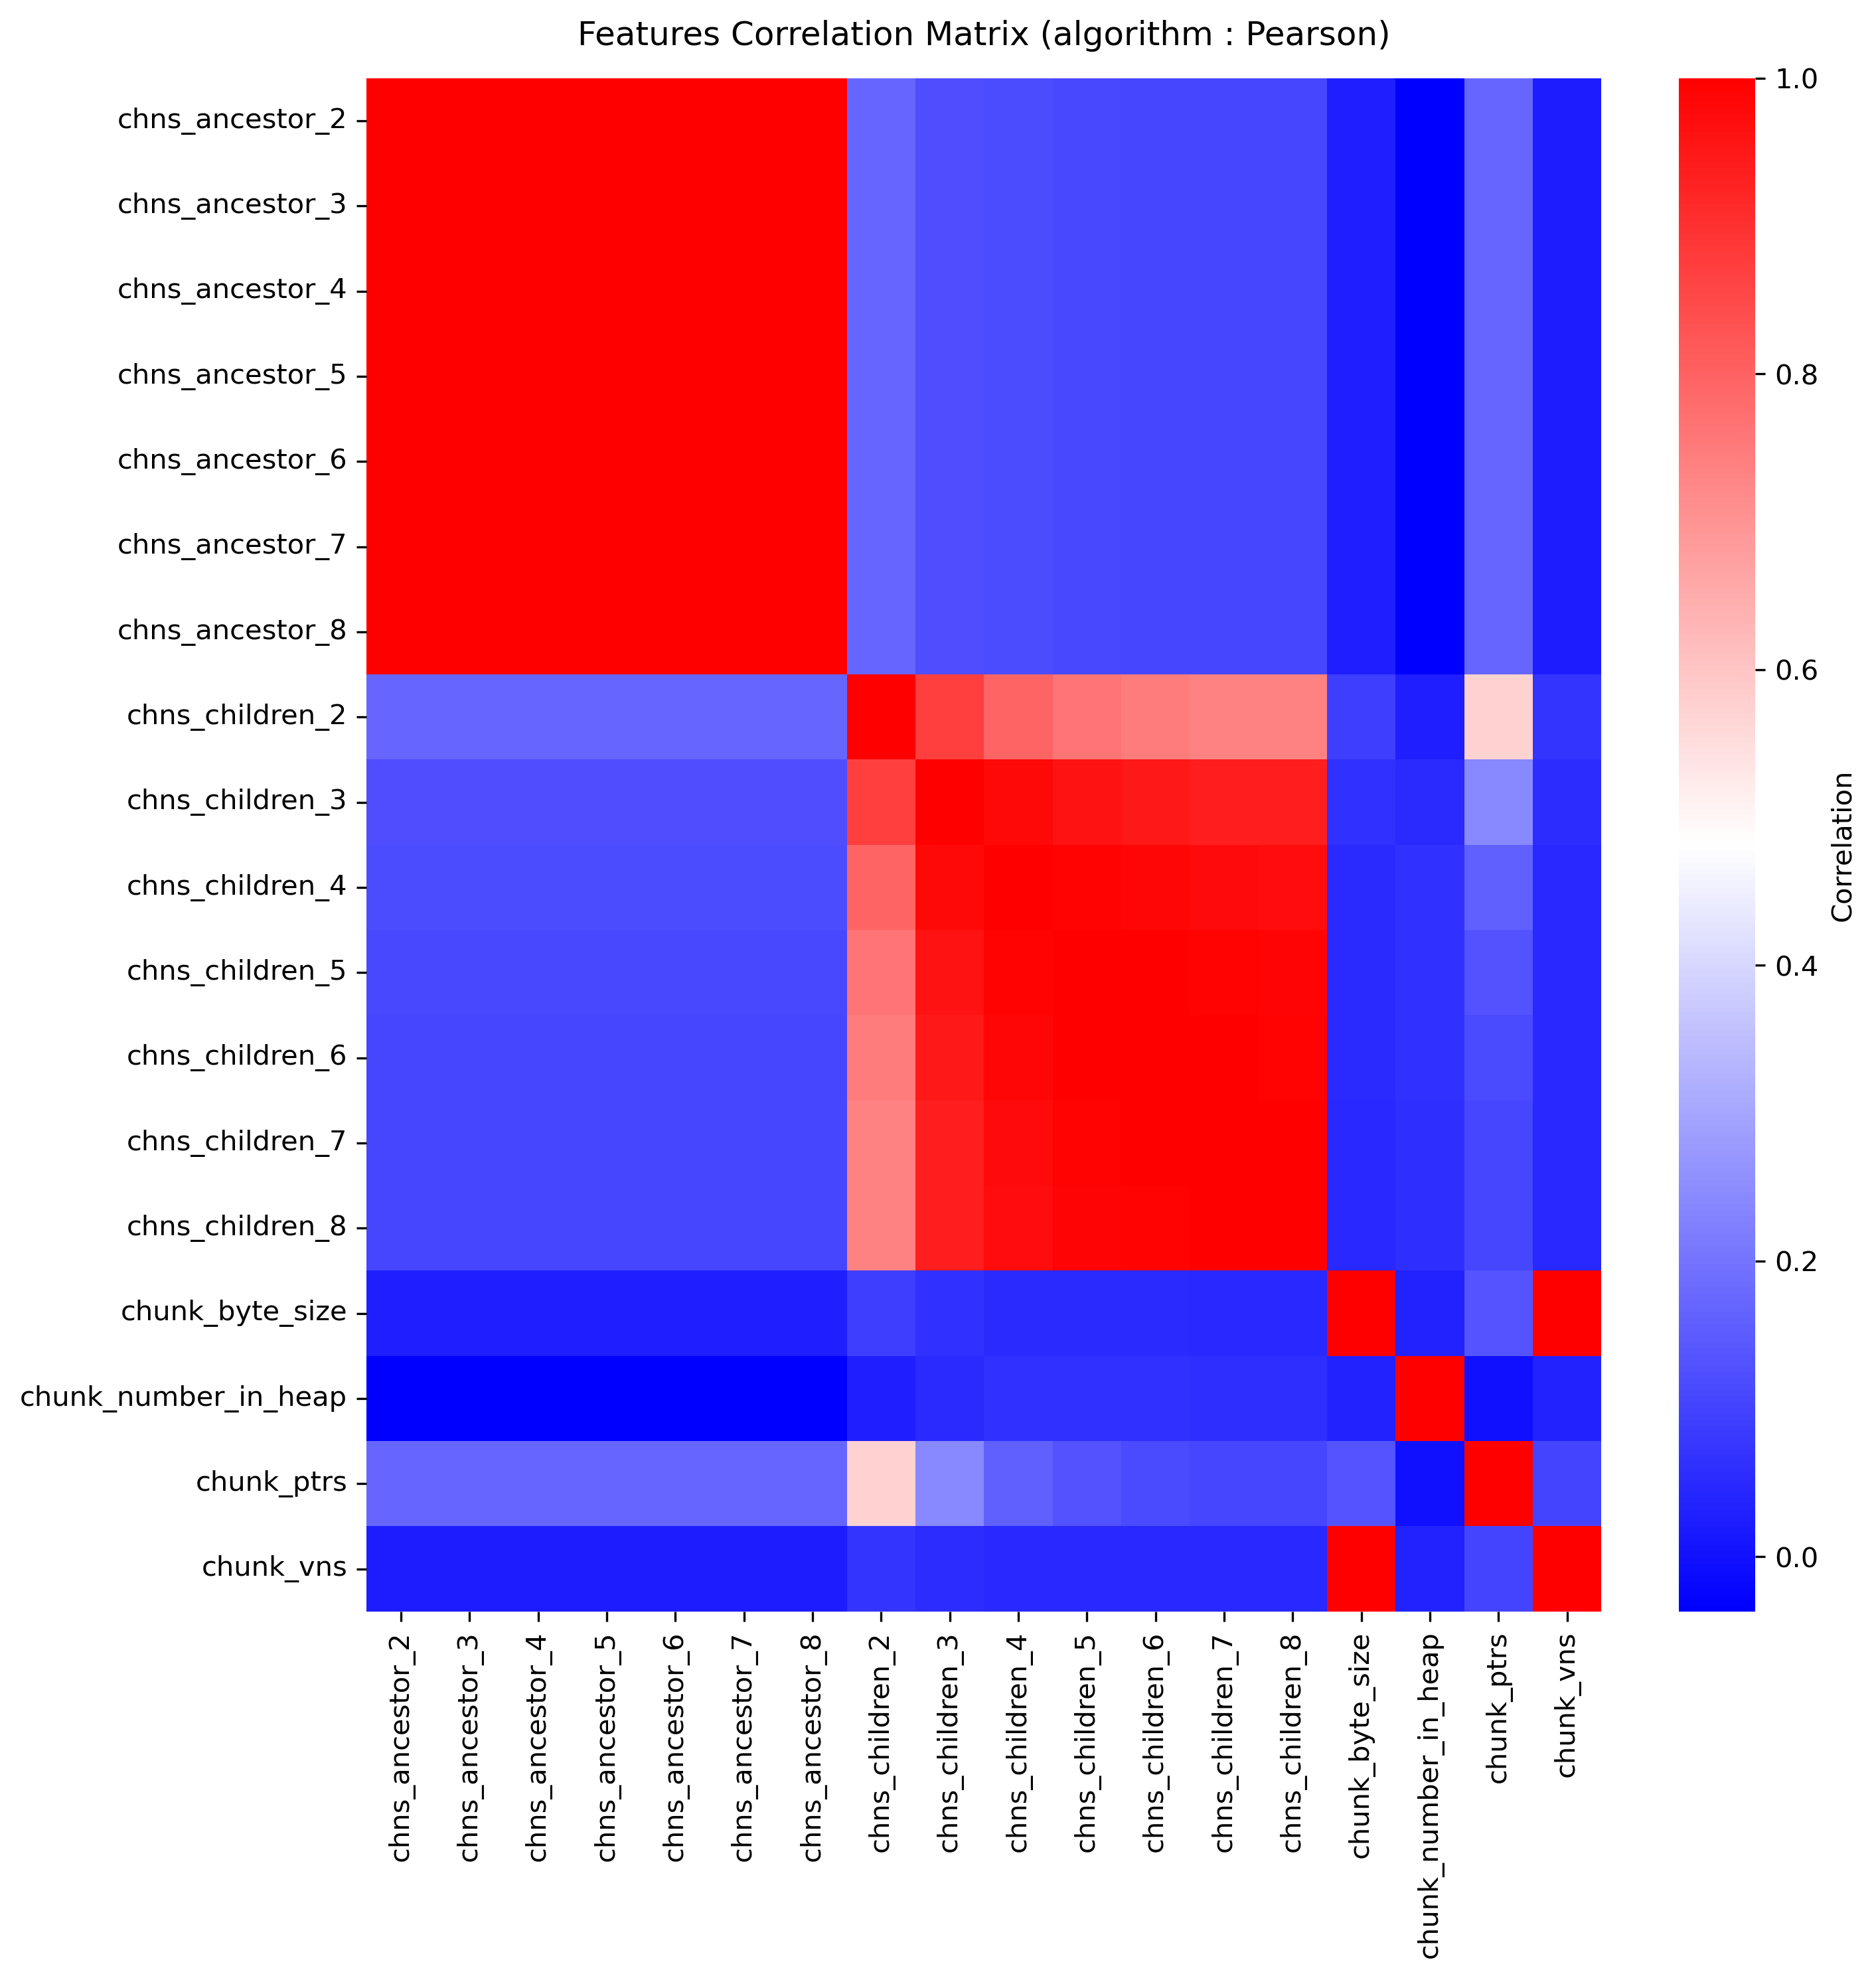
\includegraphics[width=0.8\linewidth]{img/annexes/8/single instance_correlation_matrix.png}} \\
\hline
\end{longtable}


\subsection{9 chunk\_semantic\_embedding (filtered chunk size)}

\begin{longtable}{|c|c|}
\caption{single instance Feature Engineering Results on 9} \label{tab:9_single_instance_feature_engineering_results}\\
\hline
Dataset Name & 9 \\ \hline
Instance & single instance \\ \hline
\multirow{8}{*}{Best Features} & chunk\_number\_in\_heap \\ \cline{2-2}
 & chunk\_vns \\ \cline{2-2}
 & chunk\_byte\_size \\ \cline{2-2}
 & chunk\_ptrs \\ \cline{2-2}
 & chns\_children\_8 \\ \cline{2-2}
 & chns\_children\_7 \\ \cline{2-2}
 & chns\_children\_6 \\ \cline{2-2}
 & chns\_children\_5 \\ \cline{2-2}
\noalign{\vskip 5mm}
\multicolumn{2}{|c|}{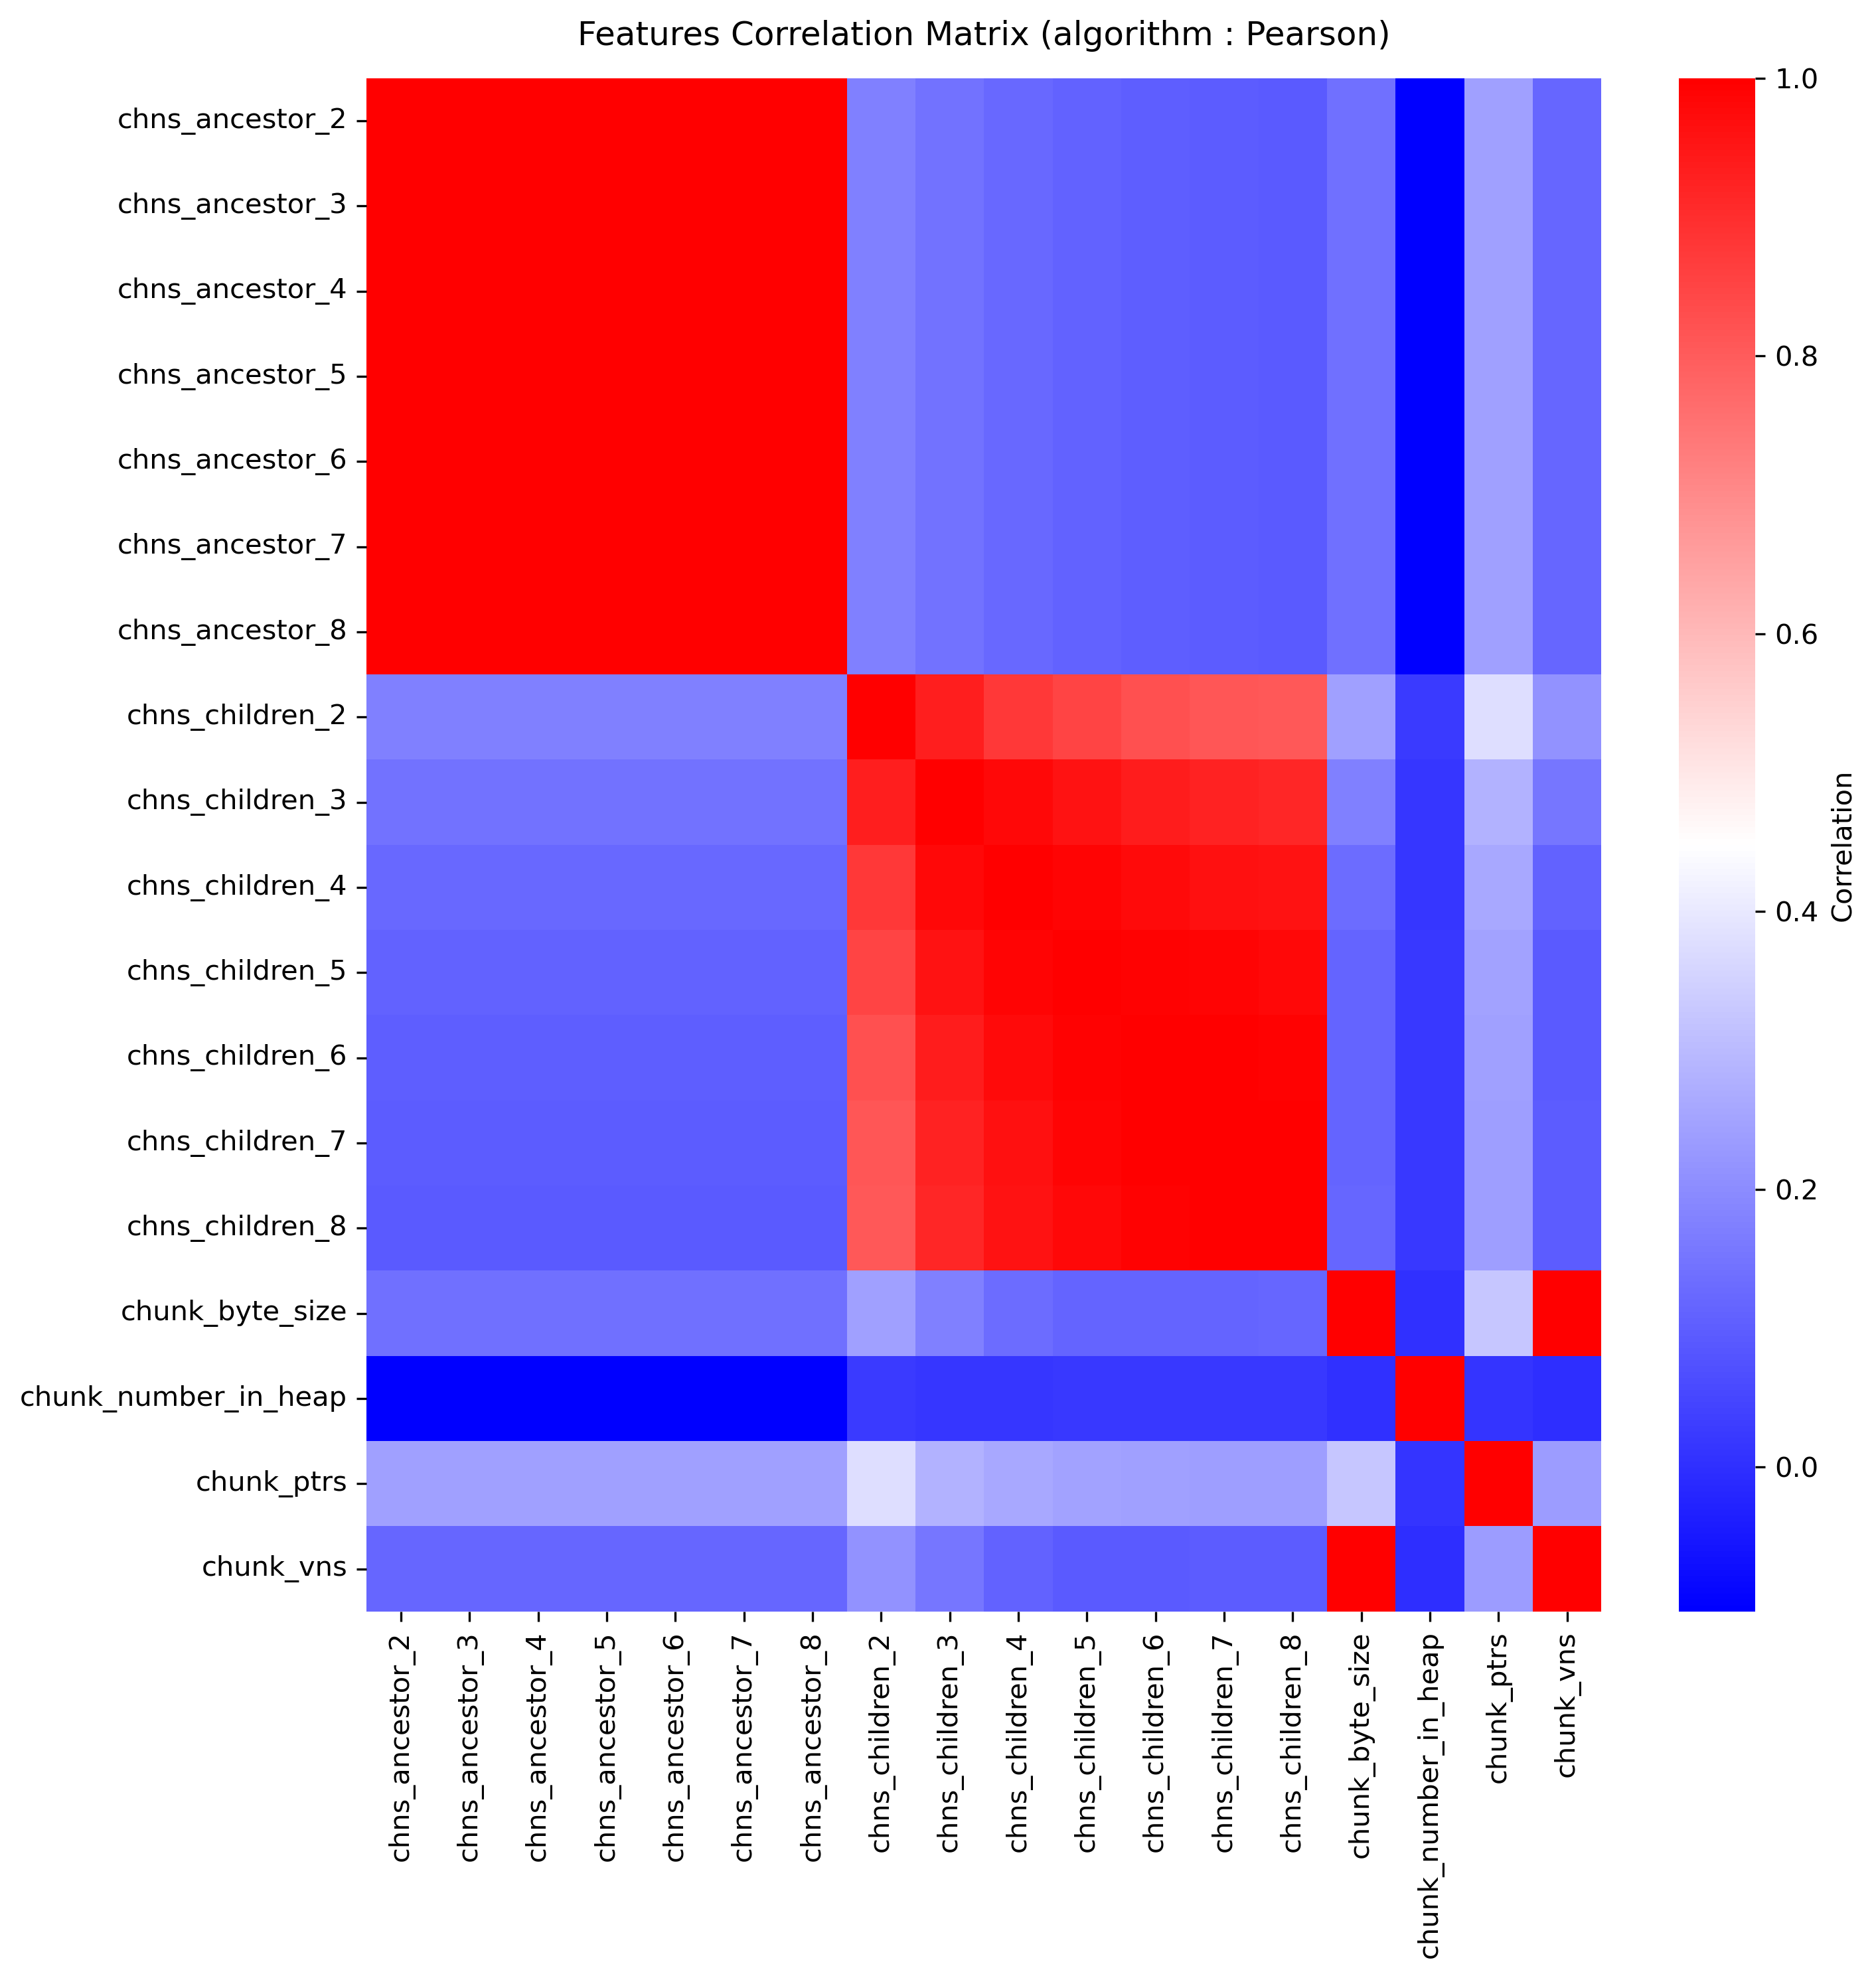
\includegraphics[width=0.8\linewidth]{img/annexes/9/single instance_correlation_matrix.png}} \\
\hline
\end{longtable}


\subsection{10 chunk\_semantic\_embedding (filtered entropy)}

\begin{longtable}{|c|c|}
\caption{single instance Feature Engineering Results on 10} \label{tab:10_single_instance_feature_engineering_results}\\
\hline
Dataset Name & 10 \\ \hline
Instance & single instance \\ \hline
\multirow{8}{*}{Best Features} & chunk\_number\_in\_heap \\ \cline{2-2}
 & chunk\_vns \\ \cline{2-2}
 & chunk\_byte\_size \\ \cline{2-2}
 & chns\_children\_8 \\ \cline{2-2}
 & chns\_children\_7 \\ \cline{2-2}
 & chns\_children\_6 \\ \cline{2-2}
 & chns\_children\_2 \\ \cline{2-2}
 & chunk\_ptrs \\ \cline{2-2}
\noalign{\vskip 5mm}
\multicolumn{2}{|c|}{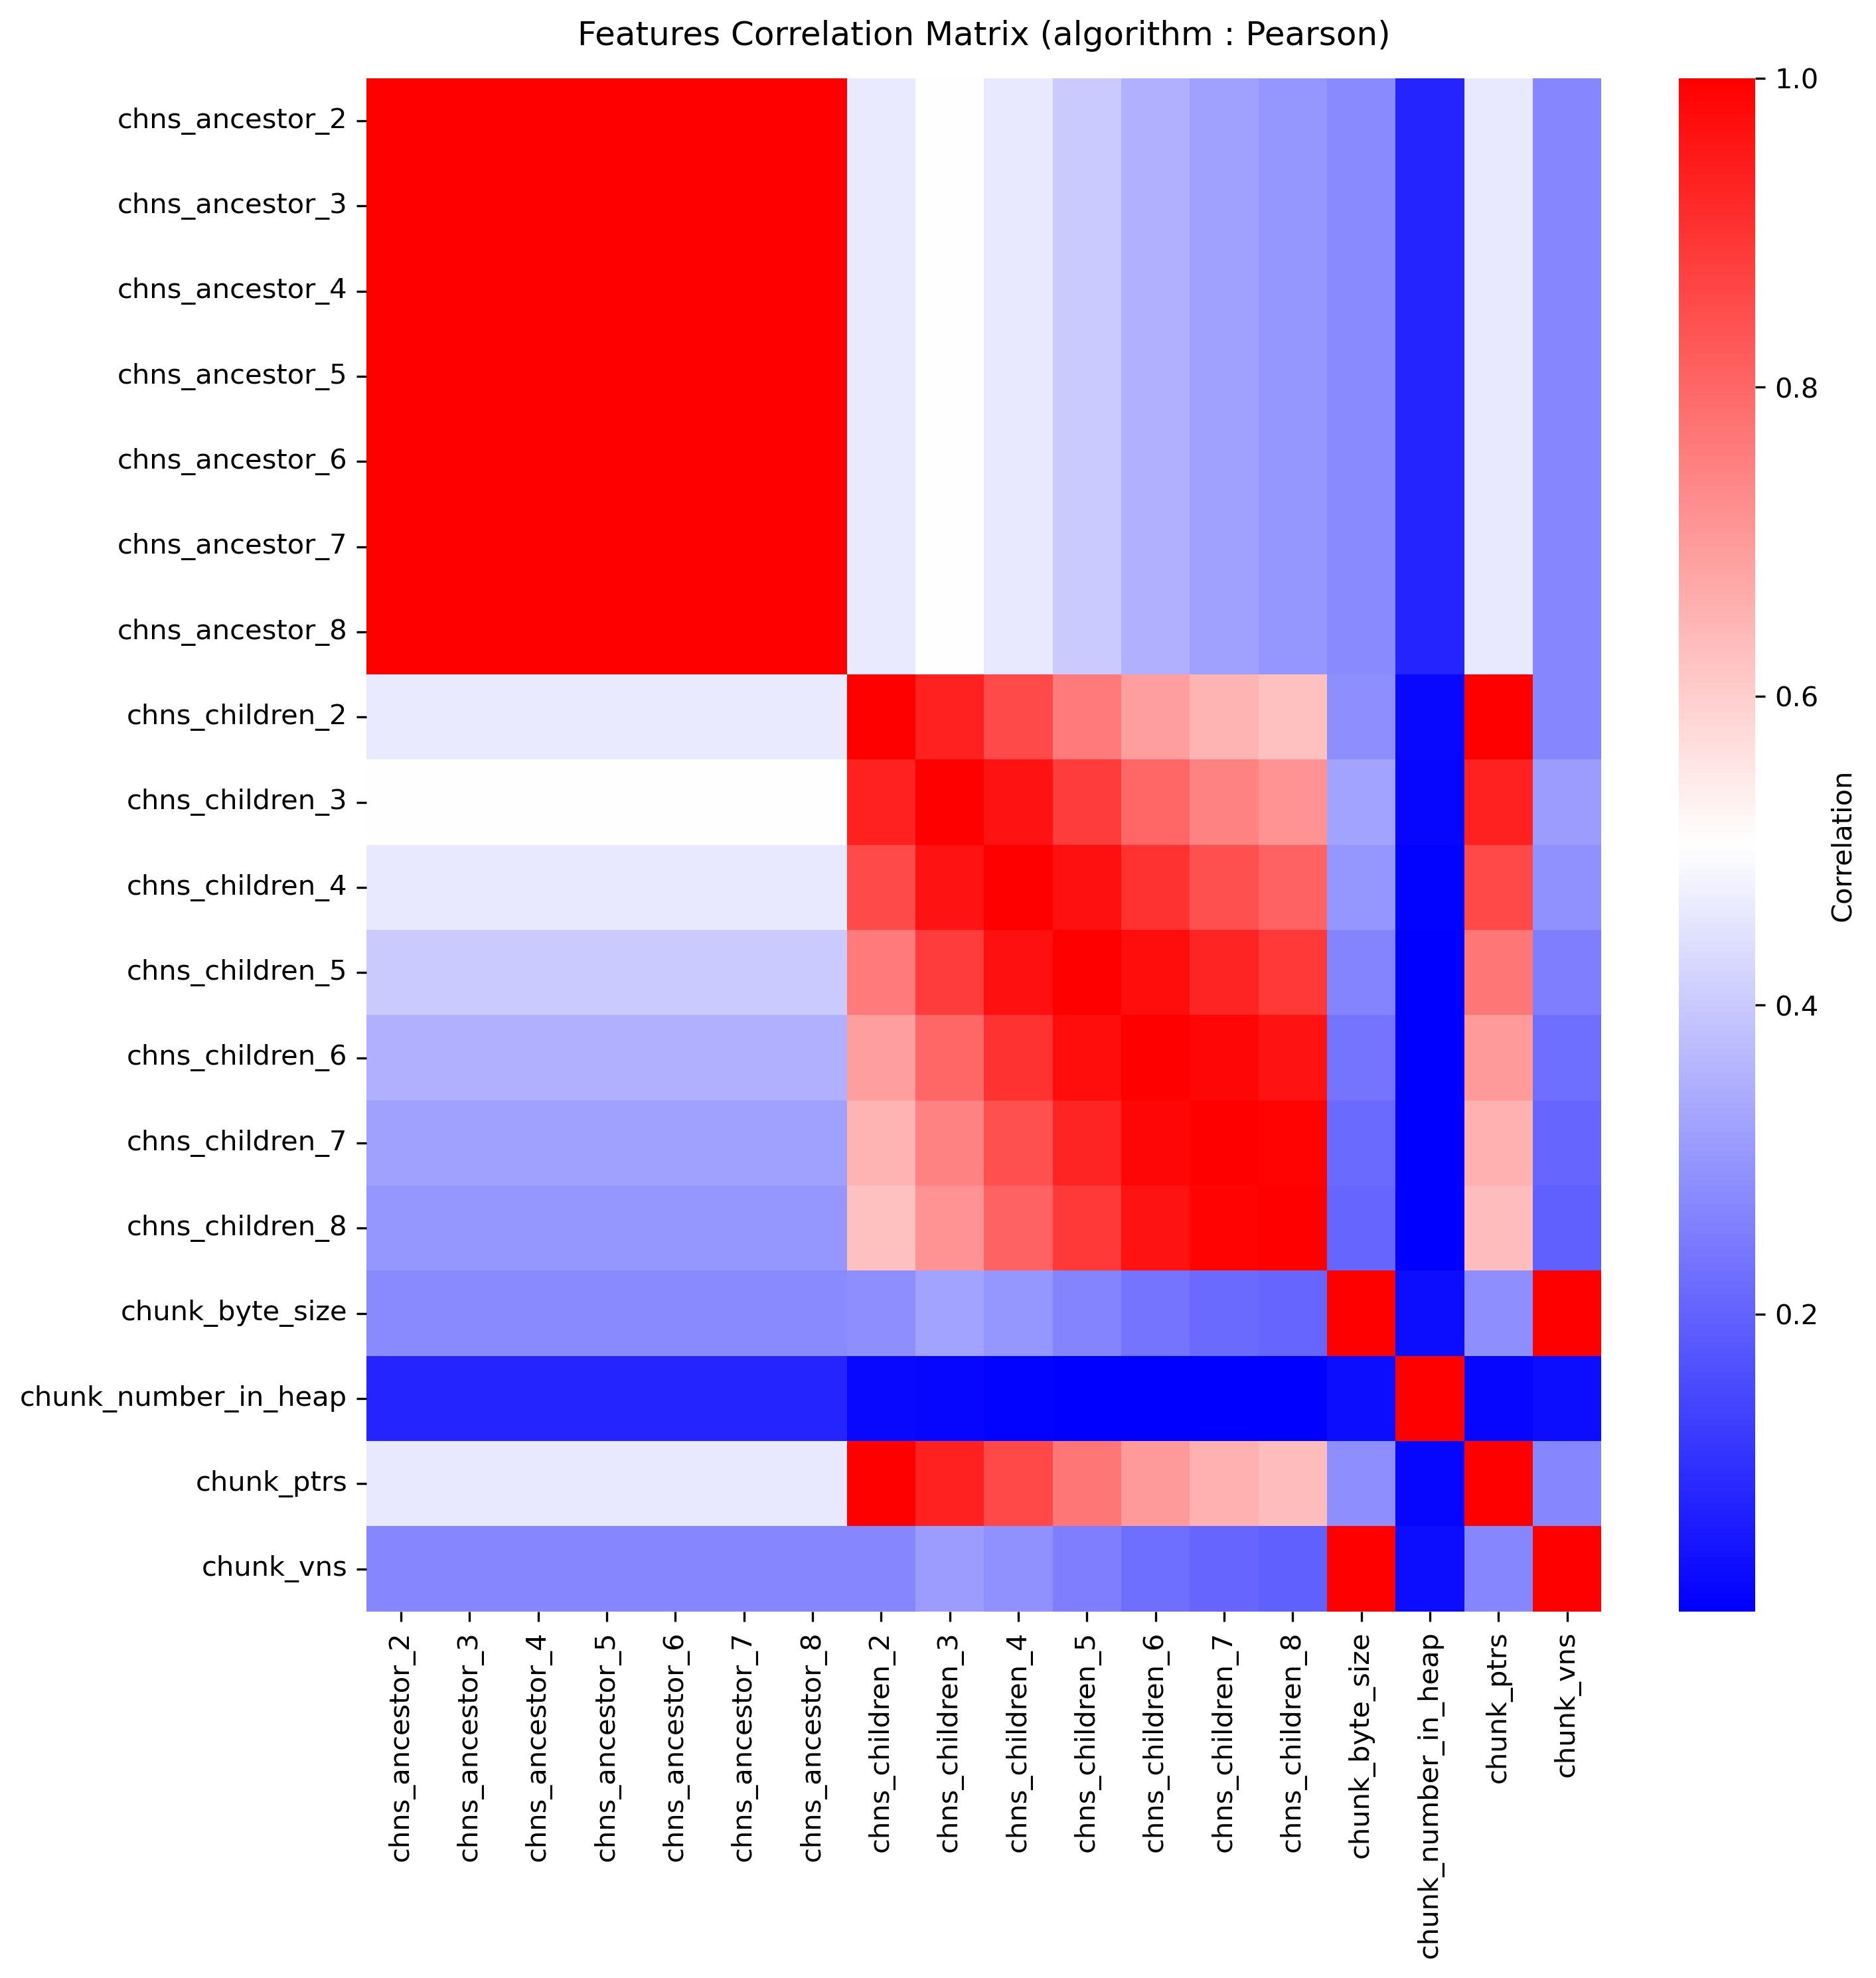
\includegraphics[width=0.8\linewidth]{img/annexes/10/single instance_correlation_matrix.png}} \\
\hline
\end{longtable}


\subsection{11 chunk\_semantic\_embedding (filtered entropy and chunk size)}

\begin{longtable}{|c|c|}
\caption{single instance Feature Engineering Results on 11} \label{tab:11_single_instance_feature_engineering_results}\\
\hline
Dataset Name & 11 \\ \hline
Instance & single instance \\ \hline
\multirow{8}{*}{Best Features} & chunk\_number\_in\_heap \\ \cline{2-2}
 & chns\_children\_8 \\ \cline{2-2}
 & chns\_children\_7 \\ \cline{2-2}
 & chns\_children\_6 \\ \cline{2-2}
 & chns\_ancestor\_2 \\ \cline{2-2}
 & chns\_ancestor\_3 \\ \cline{2-2}
 & chns\_ancestor\_4 \\ \cline{2-2}
 & chns\_ancestor\_5 \\ \cline{2-2}
\noalign{\vskip 5mm}
\multicolumn{2}{|c|}{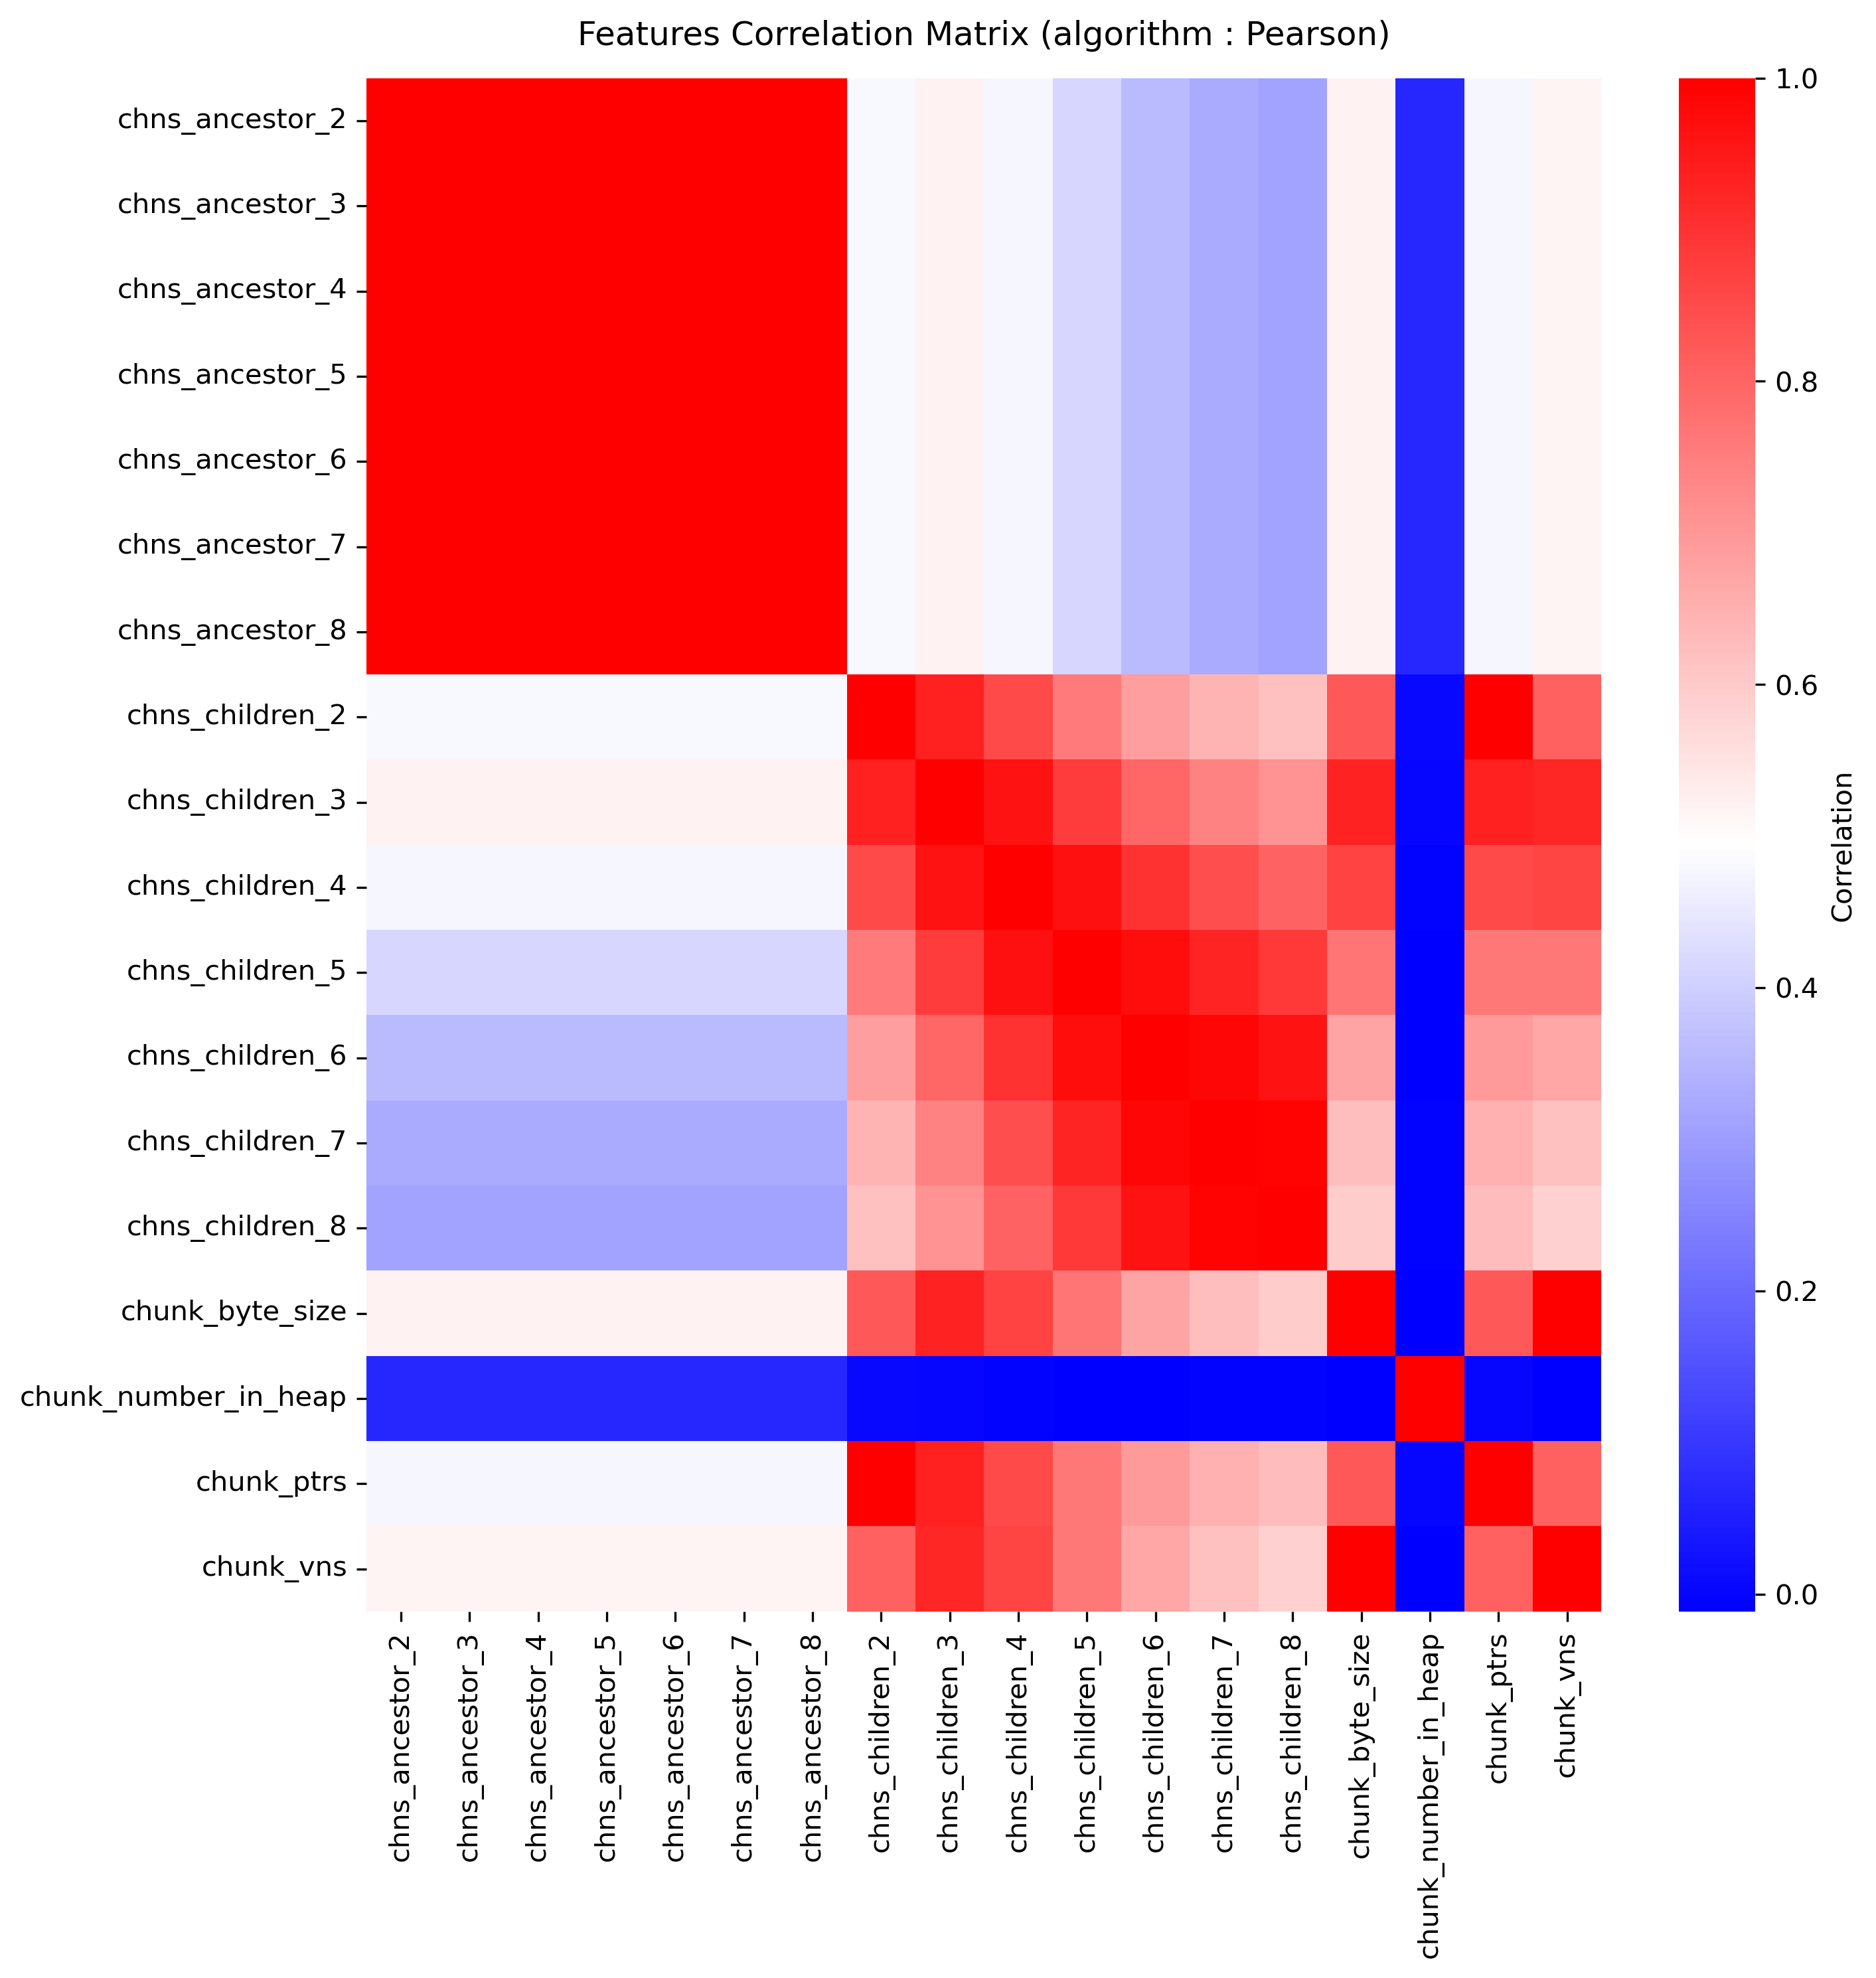
\includegraphics[width=0.8\linewidth]{img/annexes/11/single instance_correlation_matrix.png}} \\
\hline
\end{longtable}


\subsection{12 chunk\_semantic\_embedding}

\begin{longtable}{|c|c|}
\caption{single instance Feature Engineering Results on 12} \label{tab:12_single_instance_feature_engineering_results}\\
\hline
Dataset Name & 12 \\ \hline
Instance & single instance \\ \hline
\multirow{8}{*}{Best Features} & chns\_children\_3 \\ \cline{2-2}
 & chns\_children\_2 \\ \cline{2-2}
 & chunk\_number\_in\_heap \\ \cline{2-2}
 & ptrs\_children\_8 \\ \cline{2-2}
 & chunk\_vns \\ \cline{2-2}
 & chunk\_byte\_size \\ \cline{2-2}
 & ptrs\_children\_7 \\ \cline{2-2}
 & ptrs\_children\_6 \\ \cline{2-2}
\noalign{\vskip 5mm}
\multicolumn{2}{|c|}{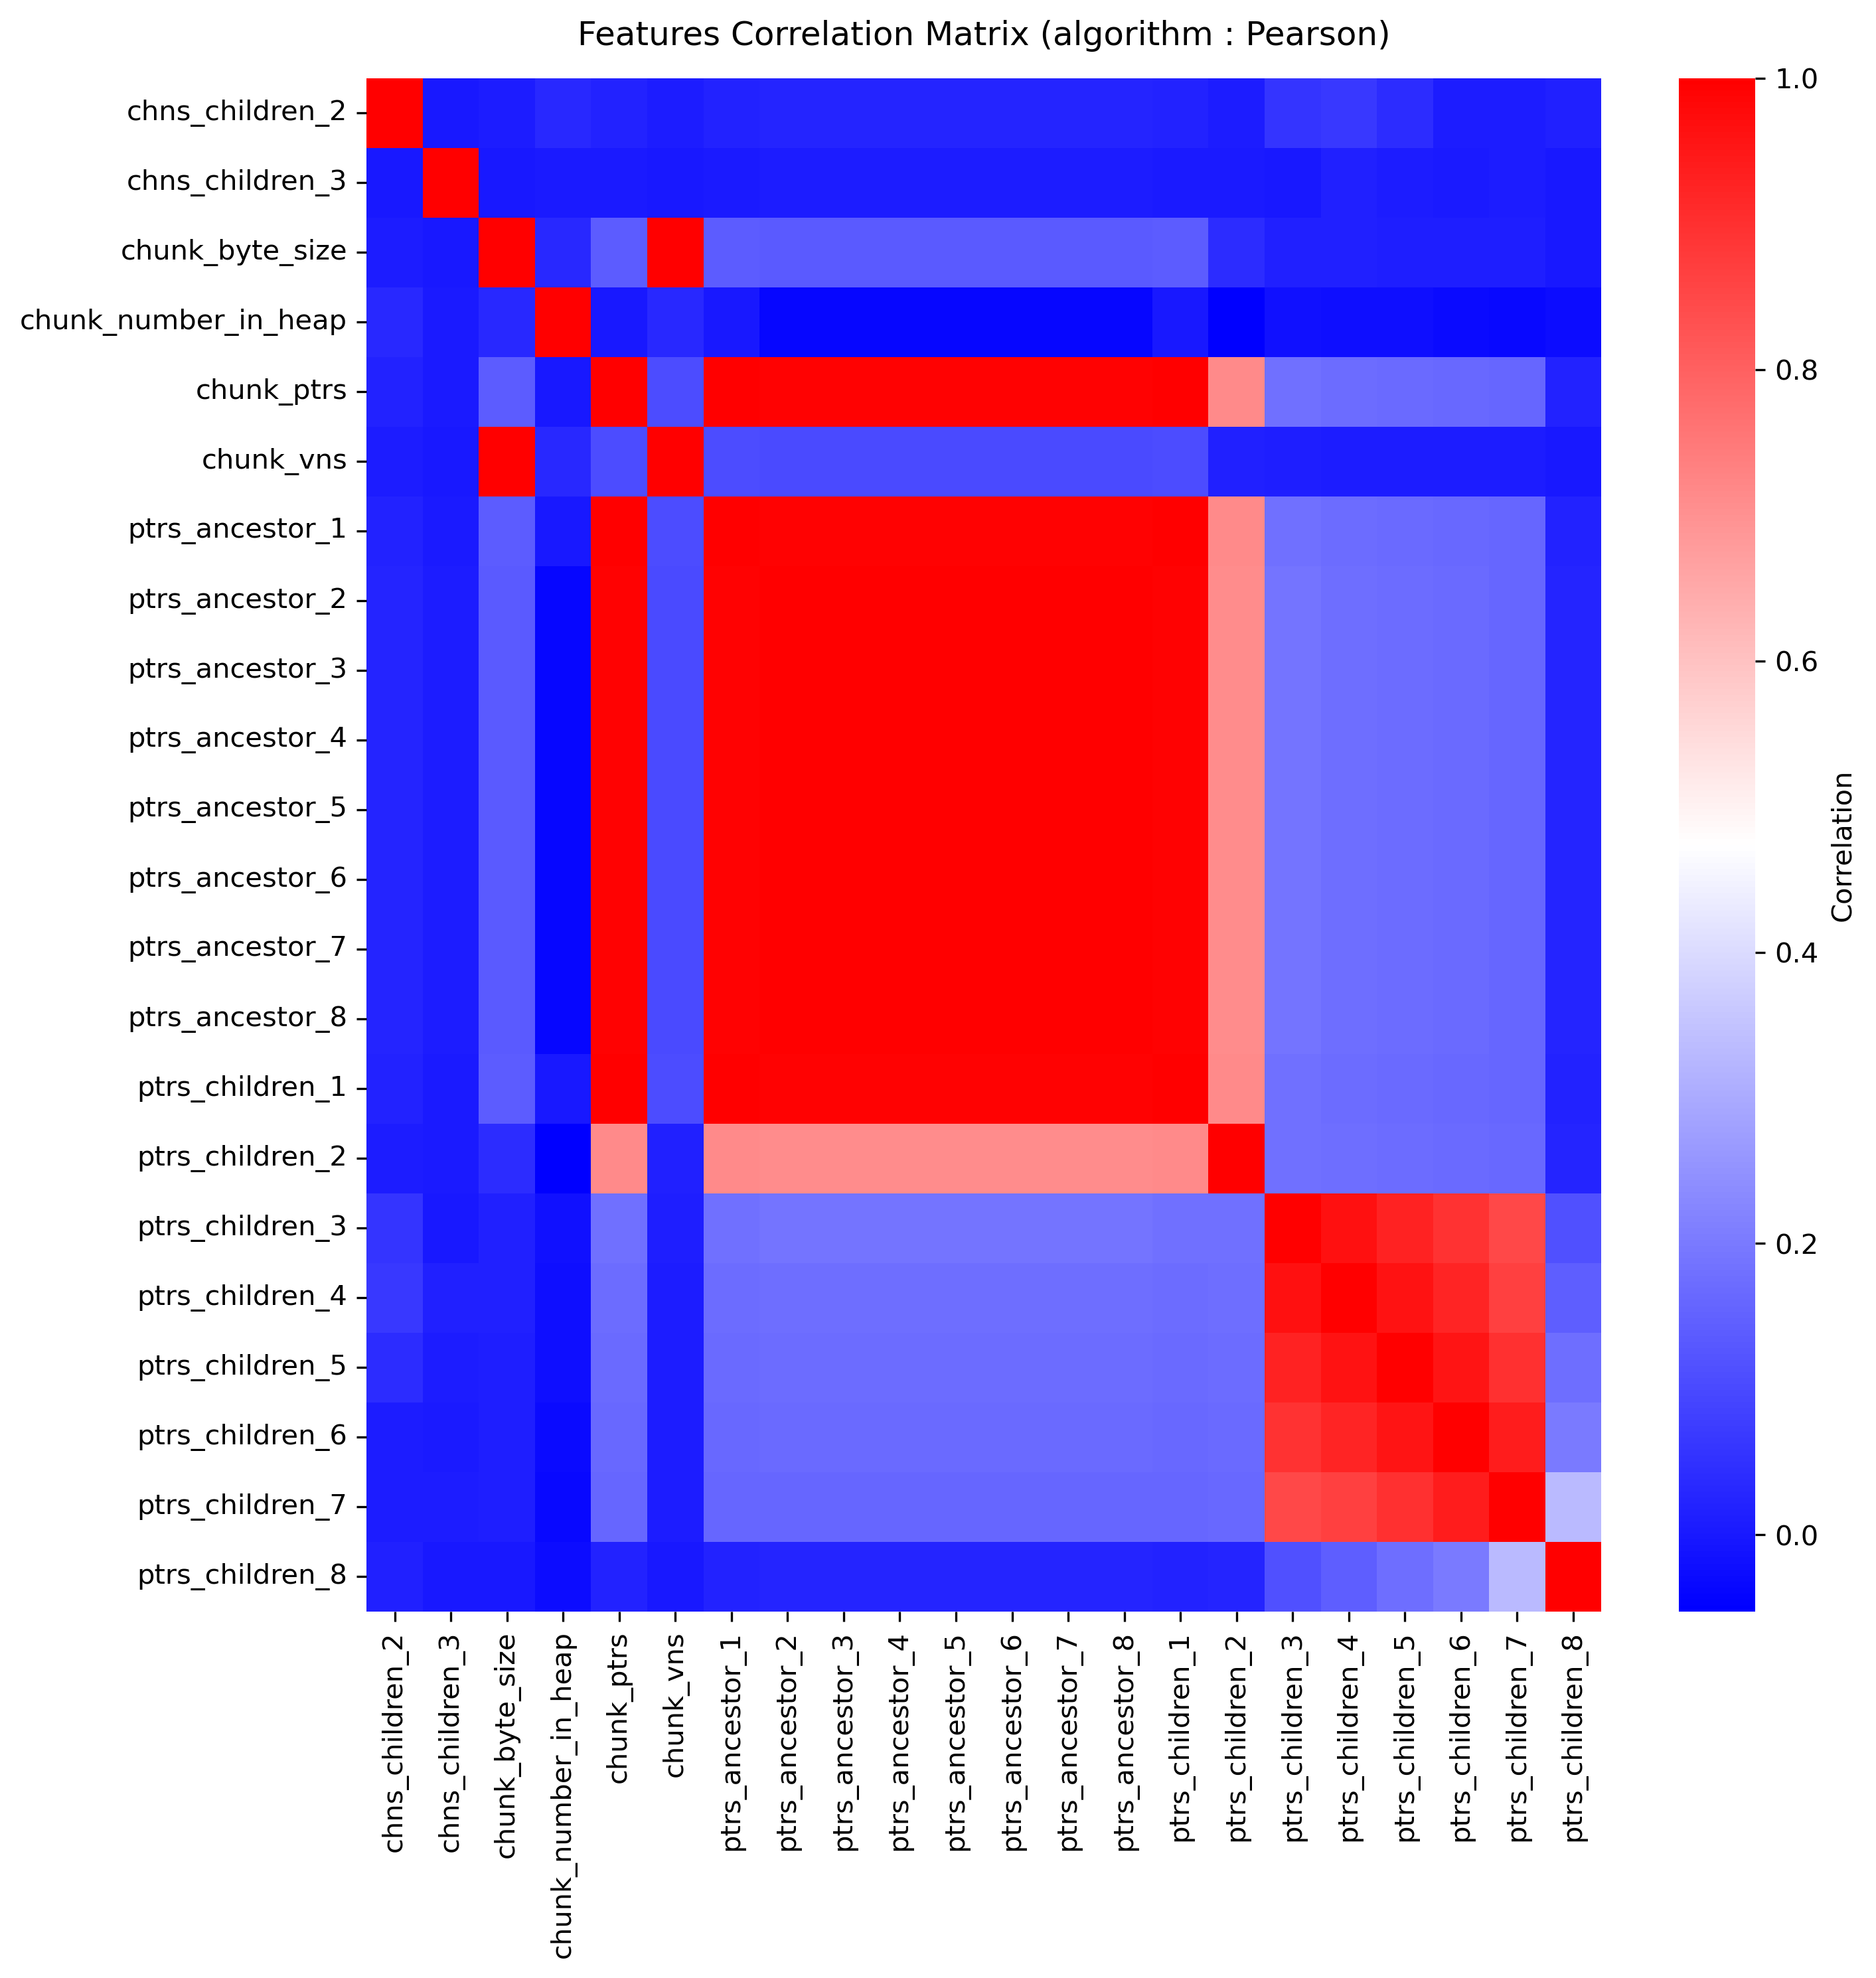
\includegraphics[width=0.8\linewidth]{img/annexes/12/single instance_correlation_matrix.png}} \\
\hline
\end{longtable}


\subsection{13 chunk\_semantic\_embedding (filtered chunk size)}

\begin{longtable}{|c|c|}
\caption{single instance Feature Engineering Results on 13} \label{tab:13_single_instance_feature_engineering_results}\\
\hline
Dataset Name & 13 \\ \hline
Instance & single instance \\ \hline
\multirow{8}{*}{Best Features} & chns\_children\_2 \\ \cline{2-2}
 & chns\_children\_3 \\ \cline{2-2}
 & chunk\_number\_in\_heap \\ \cline{2-2}
 & chunk\_vns \\ \cline{2-2}
 & chunk\_byte\_size \\ \cline{2-2}
 & ptrs\_children\_8 \\ \cline{2-2}
 & ptrs\_children\_7 \\ \cline{2-2}
 & ptrs\_children\_6 \\ \cline{2-2}
\noalign{\vskip 5mm}
\multicolumn{2}{|c|}{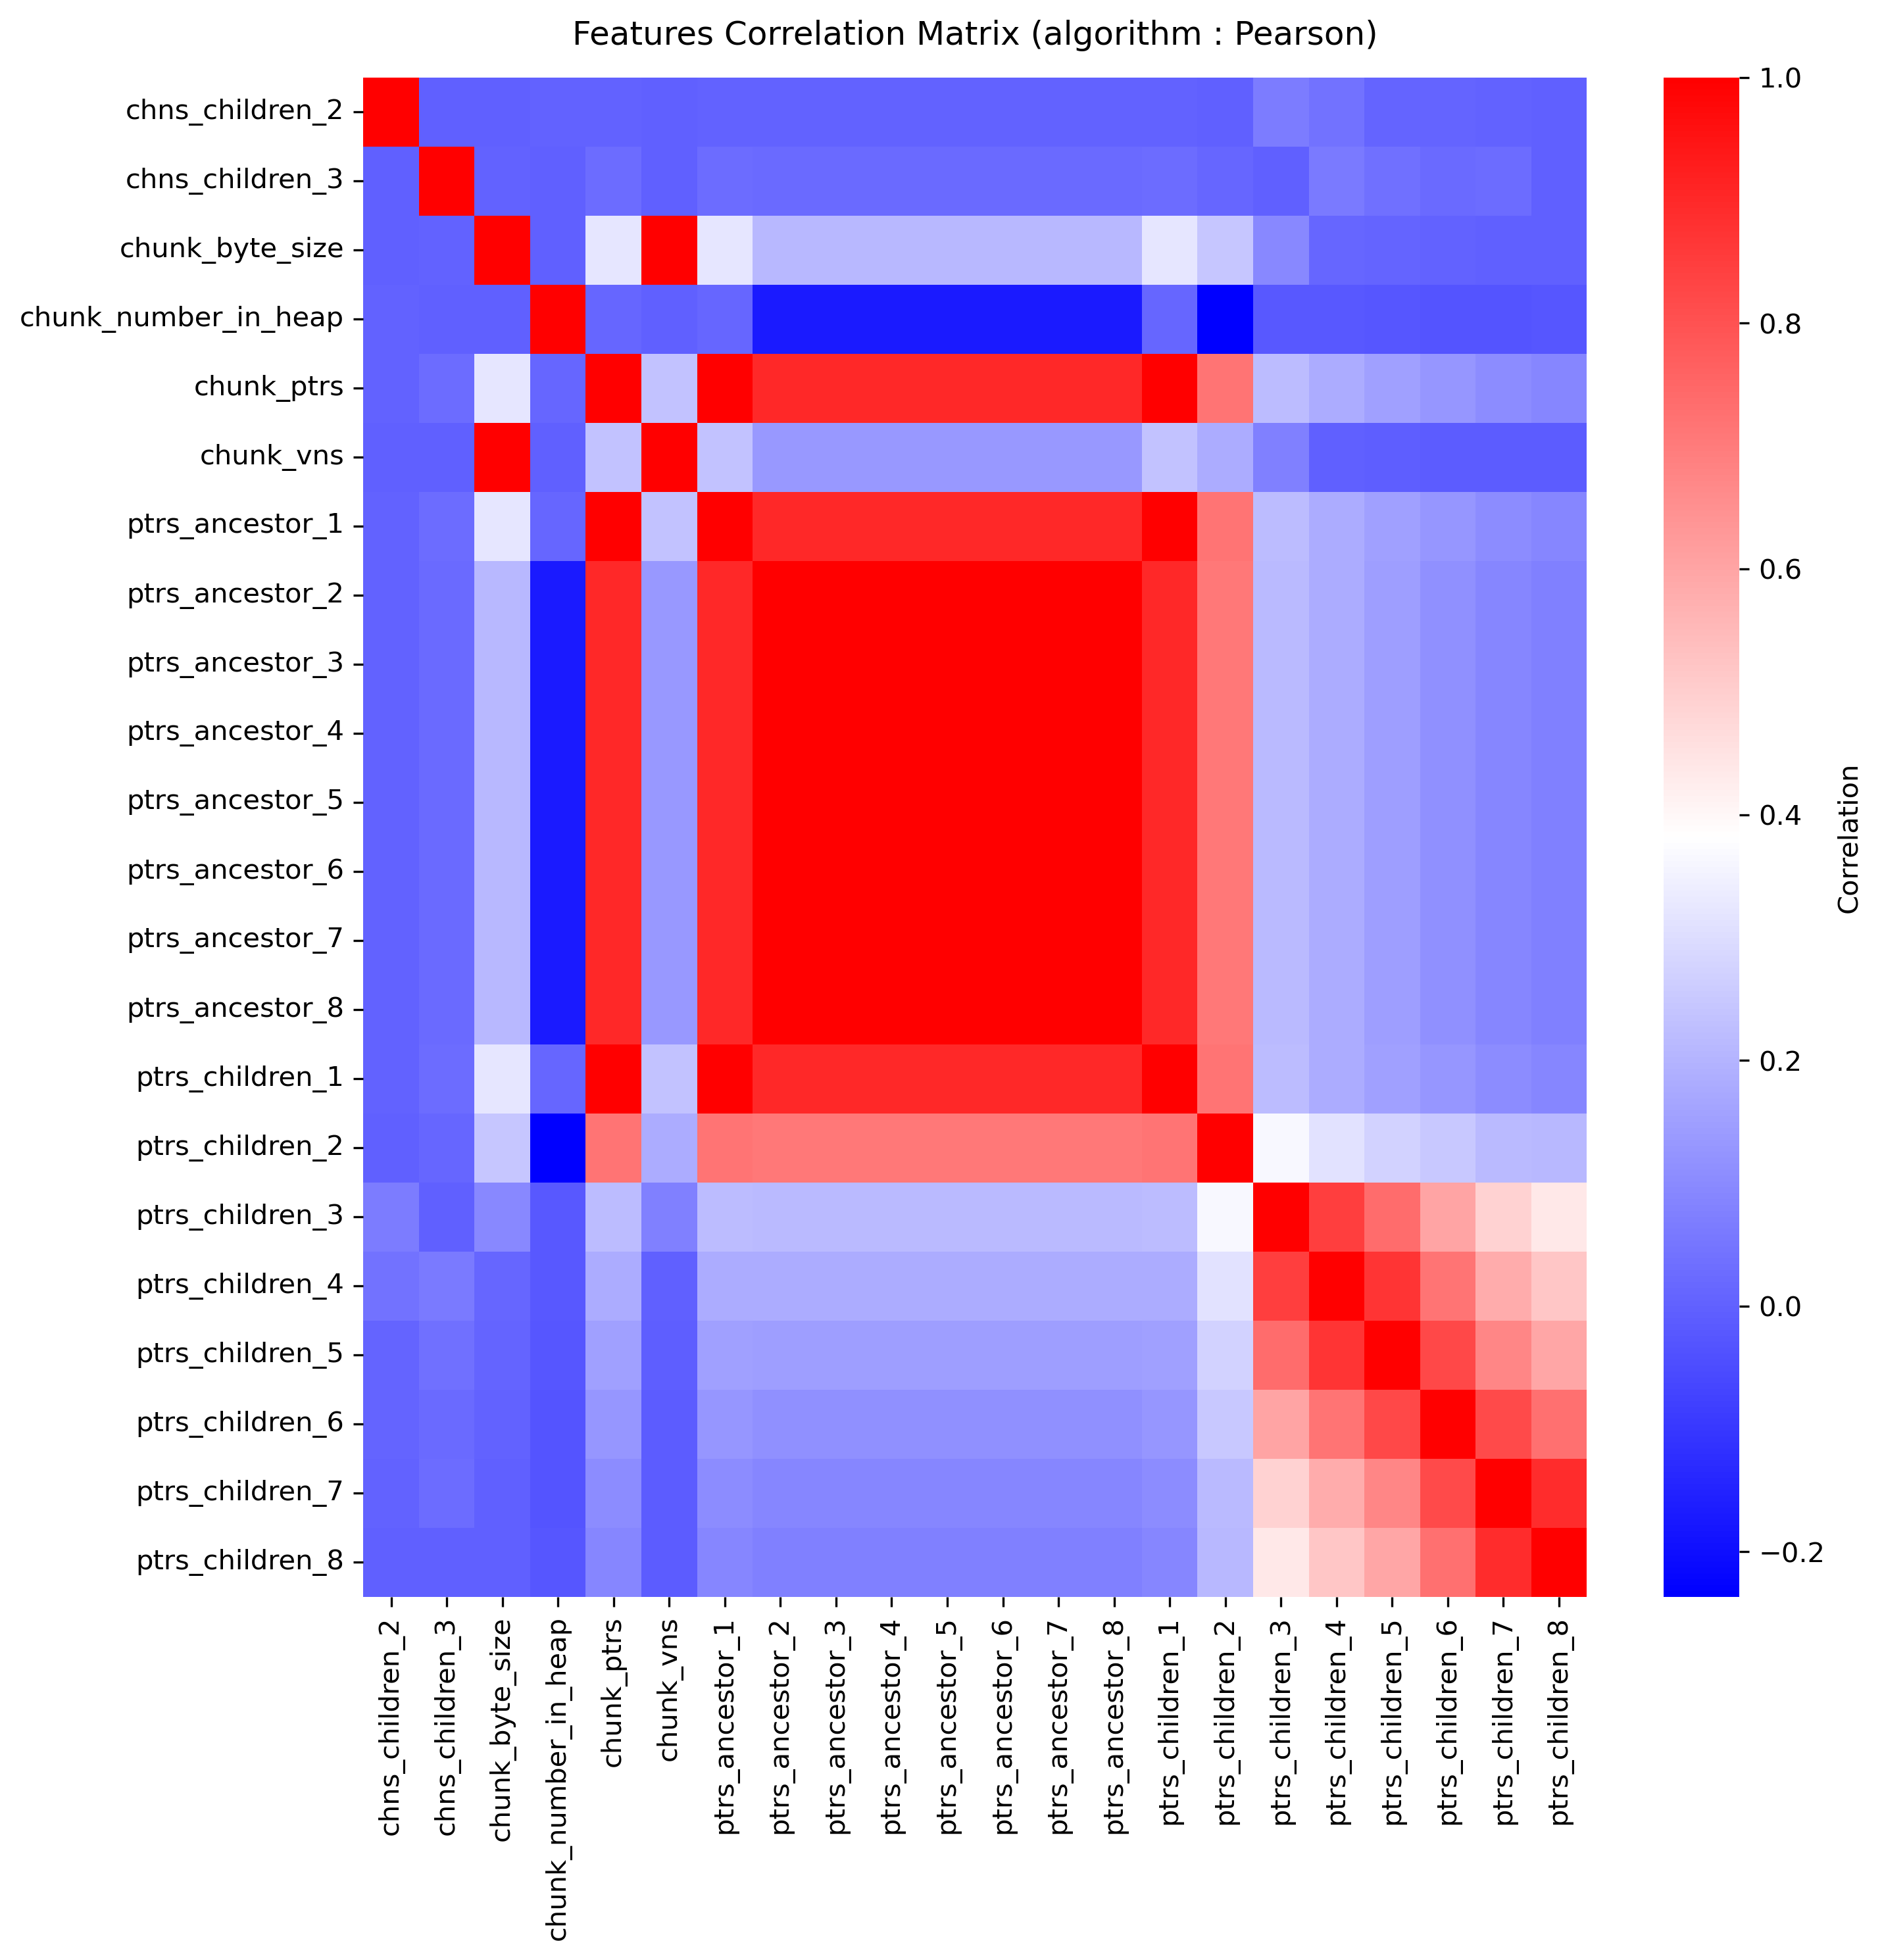
\includegraphics[width=0.8\linewidth]{img/annexes/13/single instance_correlation_matrix.png}} \\
\hline
\end{longtable}


\subsection{18 chunk\_statistic\_embedding (filtered entropy)}

\begin{longtable}{|c|c|}
\caption{single instance Feature Engineering Results on 18} \label{tab:18_single_instance_feature_engineering_results}\\
\hline
Dataset Name & 18 \\ \hline
Instance & single instance \\ \hline
\multirow{8}{*}{Best Features} & chunk\_number\_in\_heap \\ \cline{2-2}
 & kurt \\ \cline{2-2}
 & mean \\ \cline{2-2}
 & skew \\ \cline{2-2}
 & mad \\ \cline{2-2}
 & std\_dev \\ \cline{2-2}
 & 00000000 \\ \cline{2-2}
 & chunk\_ptrs \\ \cline{2-2}
\noalign{\vskip 5mm}
\multicolumn{2}{|c|}{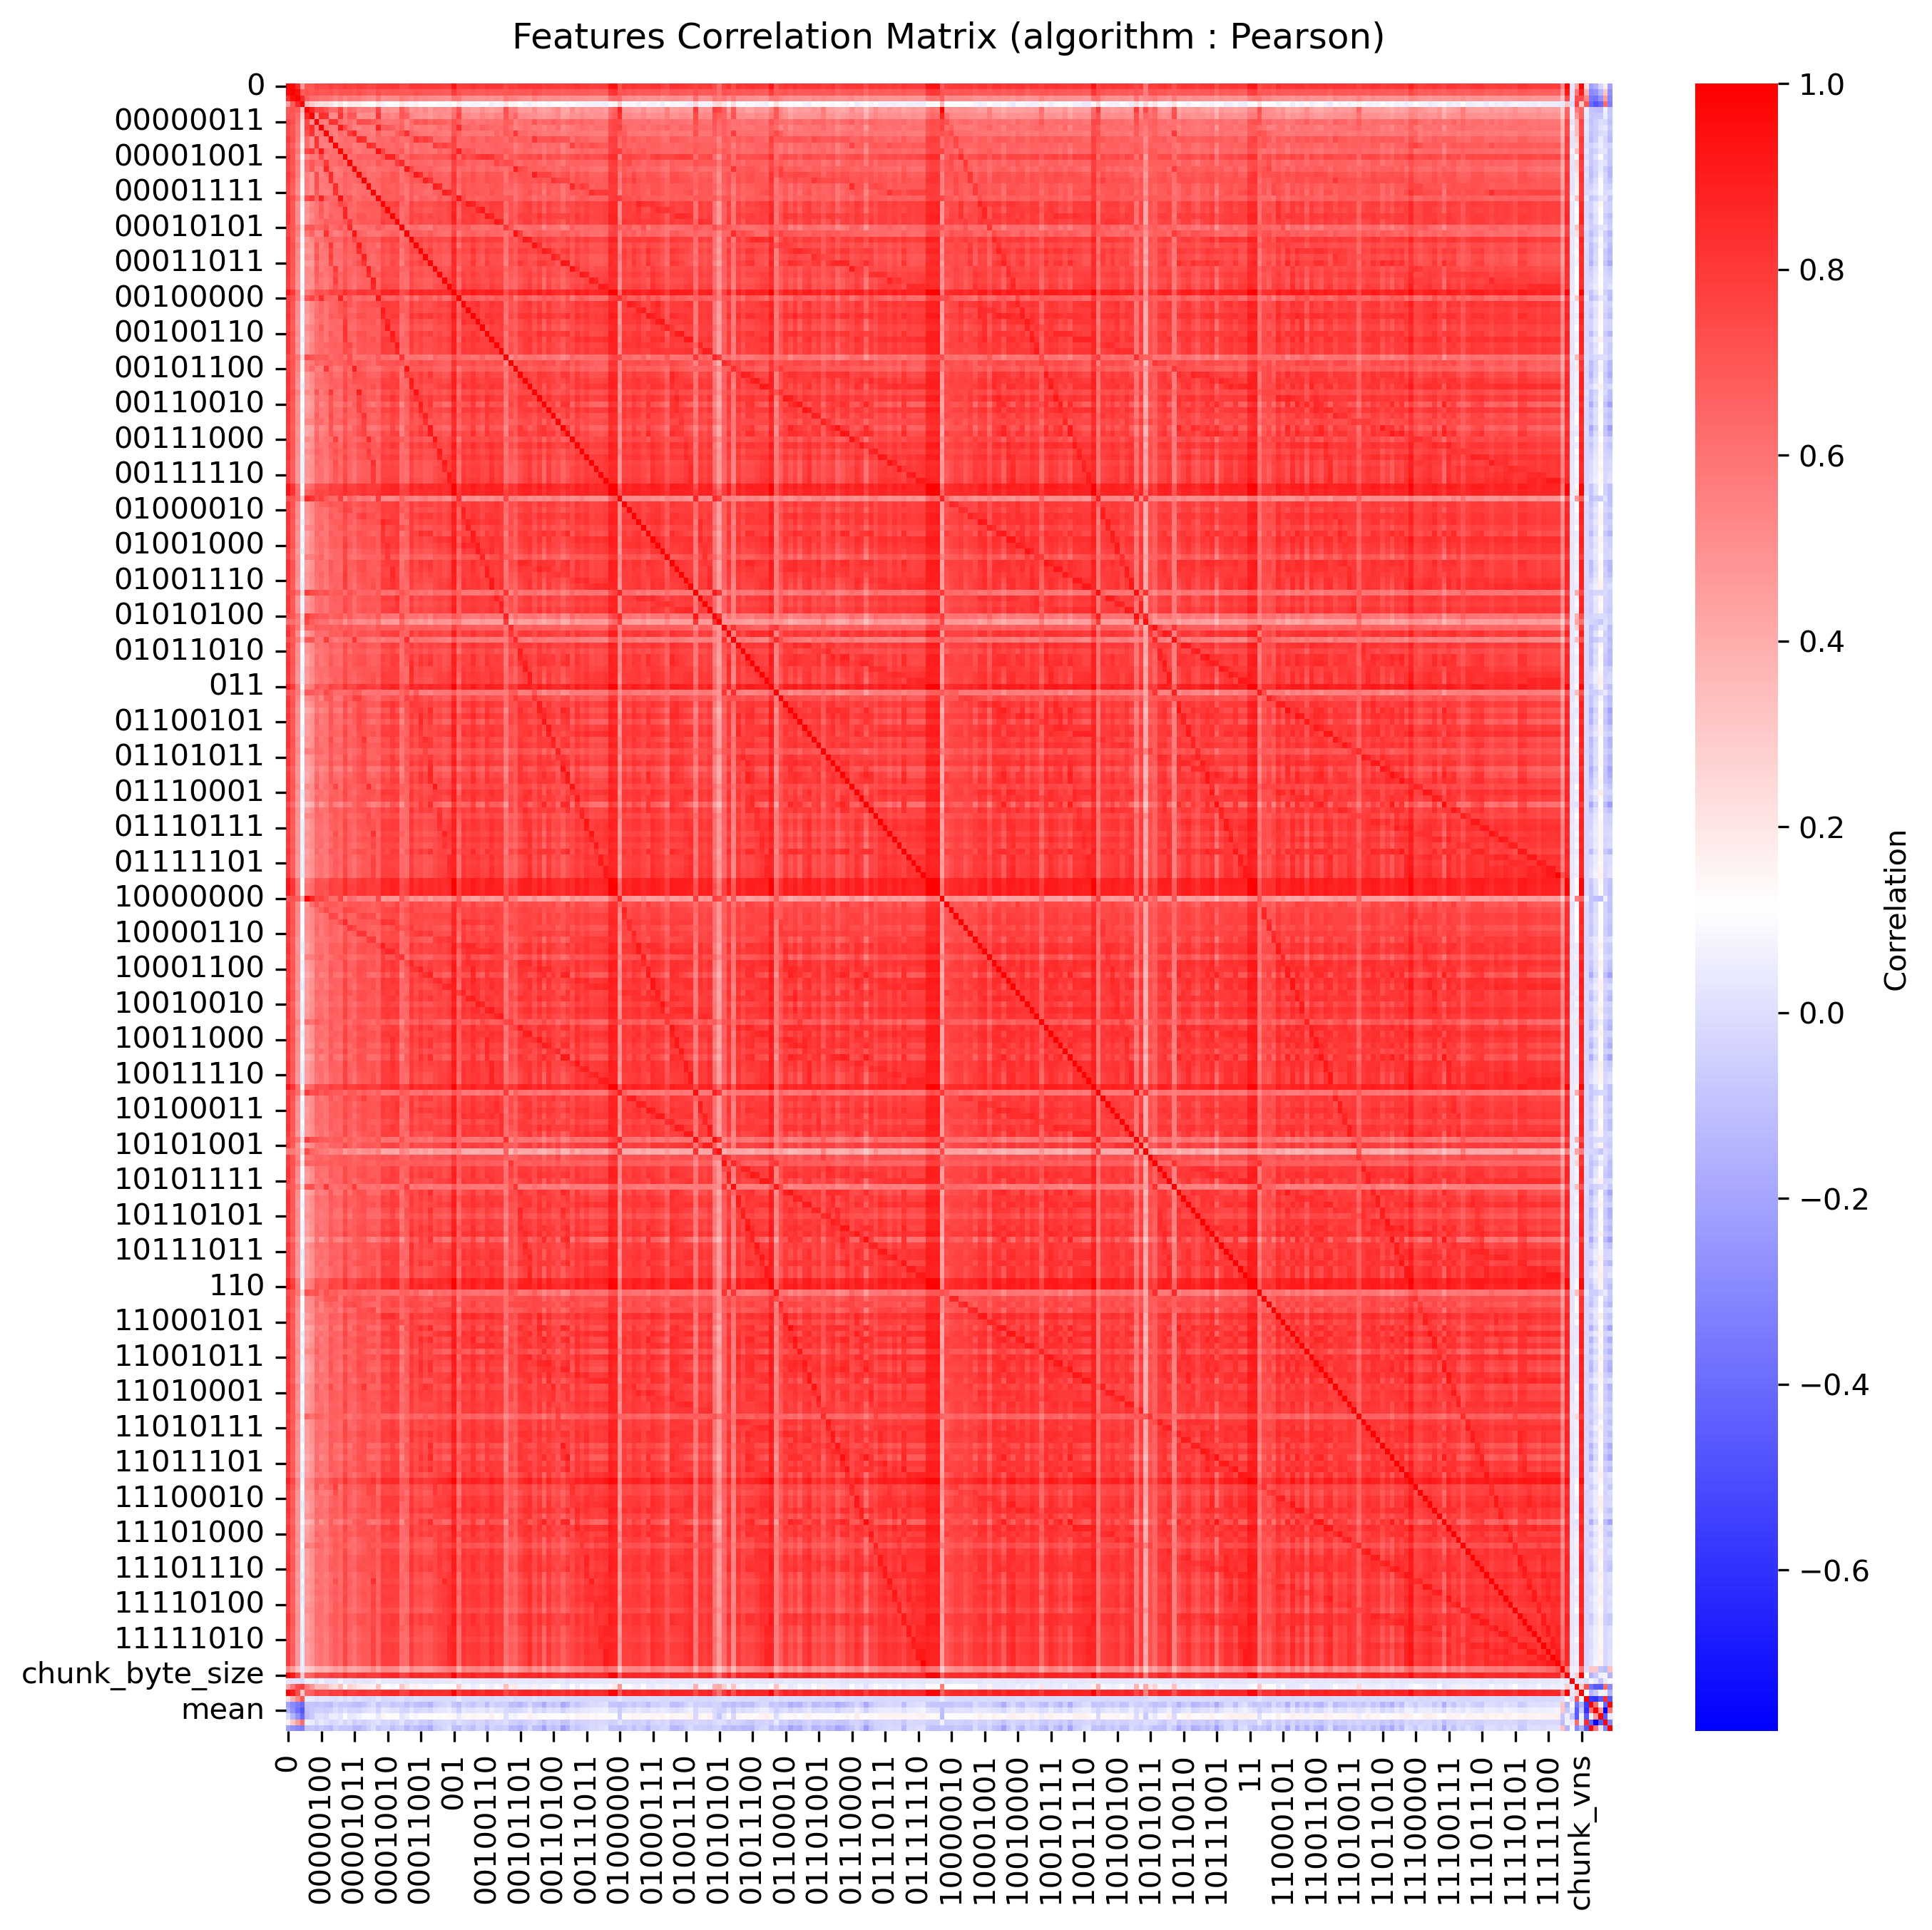
\includegraphics[width=0.8\linewidth]{img/annexes/18/single instance_correlation_matrix.png}} \\
\hline
\end{longtable}


\subsection{19 chunk\_statistic\_embedding (filtered entropy and chunk size)}

\begin{longtable}{|c|c|}
\caption{single instance Feature Engineering Results on 19} \label{tab:19_single_instance_feature_engineering_results}\\
\hline
Dataset Name & 19 \\ \hline
Instance & single instance \\ \hline
\multirow{8}{*}{Best Features} & chunk\_number\_in\_heap \\ \cline{2-2}
 & 11111111 \\ \cline{2-2}
 & kurt \\ \cline{2-2}
 & std\_dev \\ \cline{2-2}
 & skew \\ \cline{2-2}
 & mad \\ \cline{2-2}
 & mean \\ \cline{2-2}
 & 11100111 \\ \cline{2-2}
\noalign{\vskip 5mm}
\multicolumn{2}{|c|}{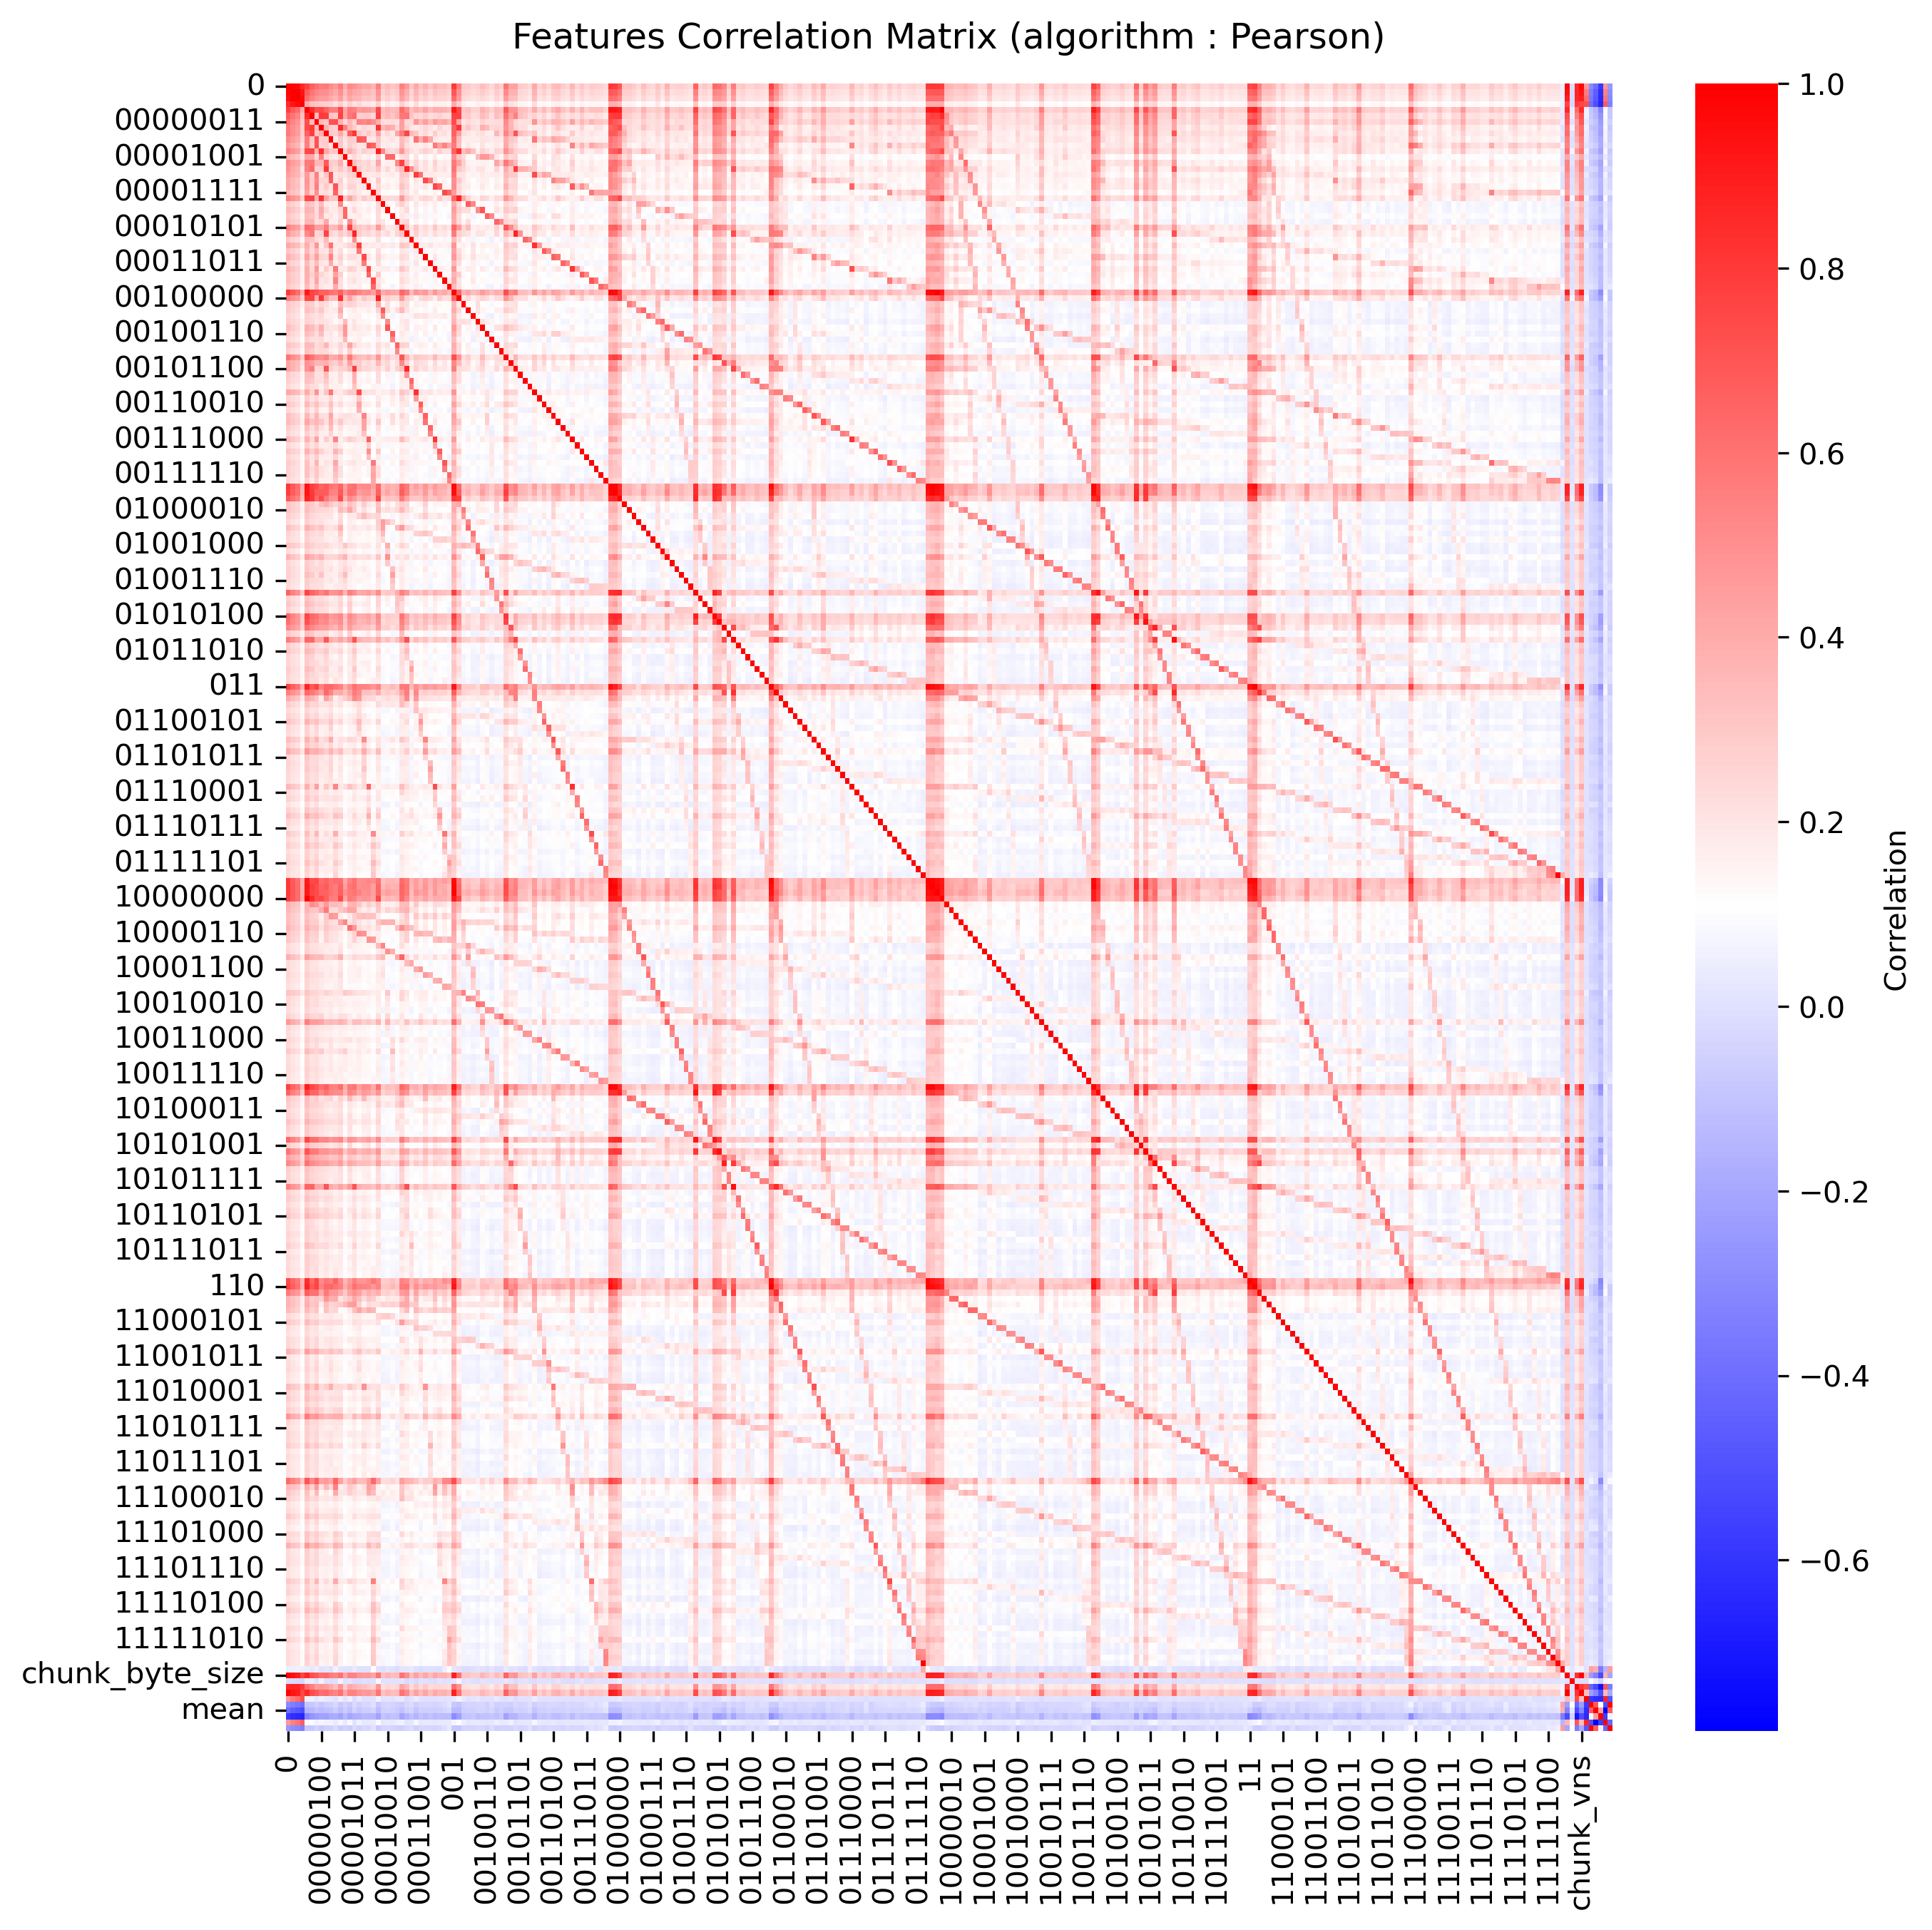
\includegraphics[width=0.8\linewidth]{img/annexes/19/single instance_correlation_matrix.png}} \\
\hline
\end{longtable}


\subsection{20 chunk\_start\_bytes\_embedding}

\begin{longtable}{|c|c|}
\caption{single instance Feature Engineering Results on 20} \label{tab:20_single_instance_feature_engineering_results}\\
\hline
Dataset Name & 20 \\ \hline
Instance & single instance \\ \hline
\multirow{8}{*}{Best Features} & chunk\_ptrs \\ \cline{2-2}
 & chunk\_vns \\ \cline{2-2}
 & chunk\_byte\_size \\ \cline{2-2}
 & byte\_11 \\ \cline{2-2}
 & byte\_10 \\ \cline{2-2}
 & byte\_7 \\ \cline{2-2}
 & byte\_6 \\ \cline{2-2}
 & chunk\_number\_in\_heap \\ \cline{2-2}
\noalign{\vskip 5mm}
\multicolumn{2}{|c|}{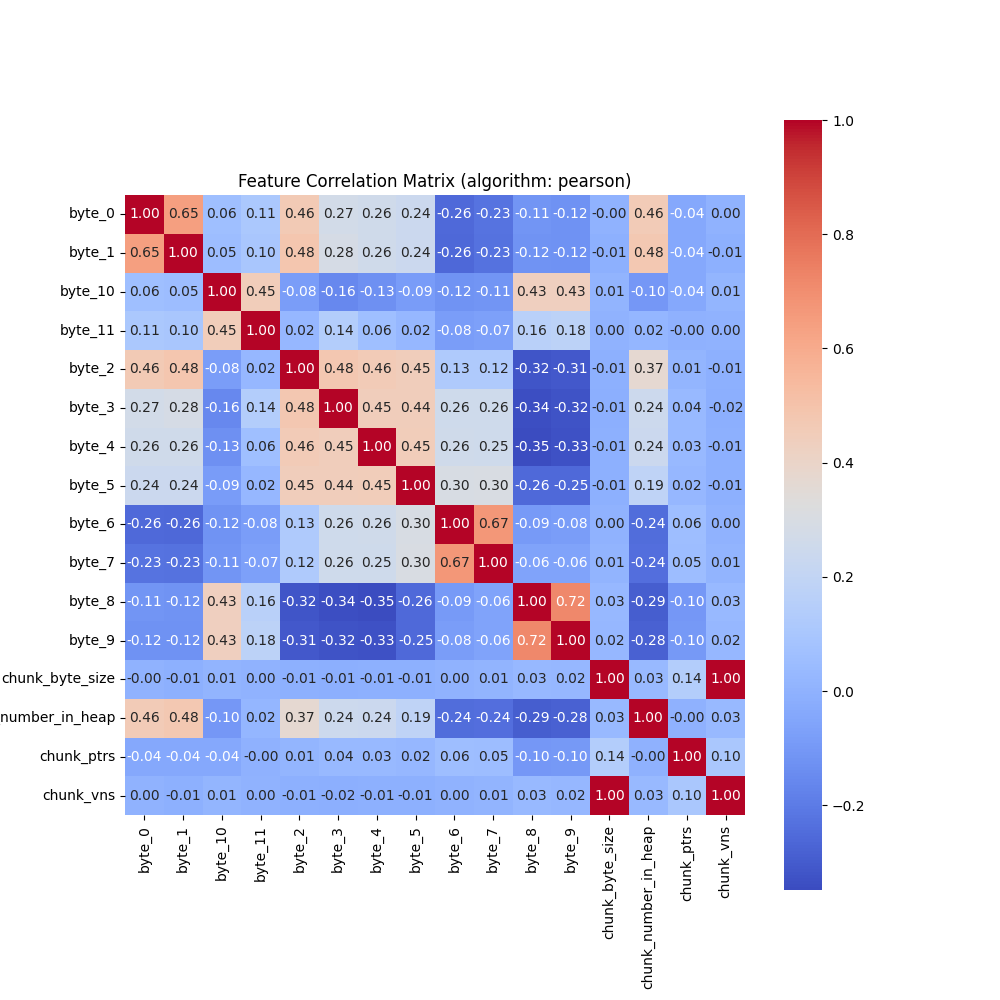
\includegraphics[width=0.8\linewidth]{img/annexes/20/single instance_correlation_matrix.png}} \\
\hline
\end{longtable}


\subsection{21 chunk\_start\_bytes\_embedding (filtered chunk size)}

\begin{longtable}{|c|c|}
\caption{single instance Feature Engineering Results on 21} \label{tab:21_single_instance_feature_engineering_results}\\
\hline
Dataset Name & 21 \\ \hline
Instance & single instance \\ \hline
\multirow{8}{*}{Best Features} & chunk\_byte\_size \\ \cline{2-2}
 & chunk\_vns \\ \cline{2-2}
 & byte\_11 \\ \cline{2-2}
 & byte\_10 \\ \cline{2-2}
 & byte\_7 \\ \cline{2-2}
 & byte\_6 \\ \cline{2-2}
 & byte\_0 \\ \cline{2-2}
 & byte\_1 \\ \cline{2-2}
\noalign{\vskip 5mm}
\multicolumn{2}{|c|}{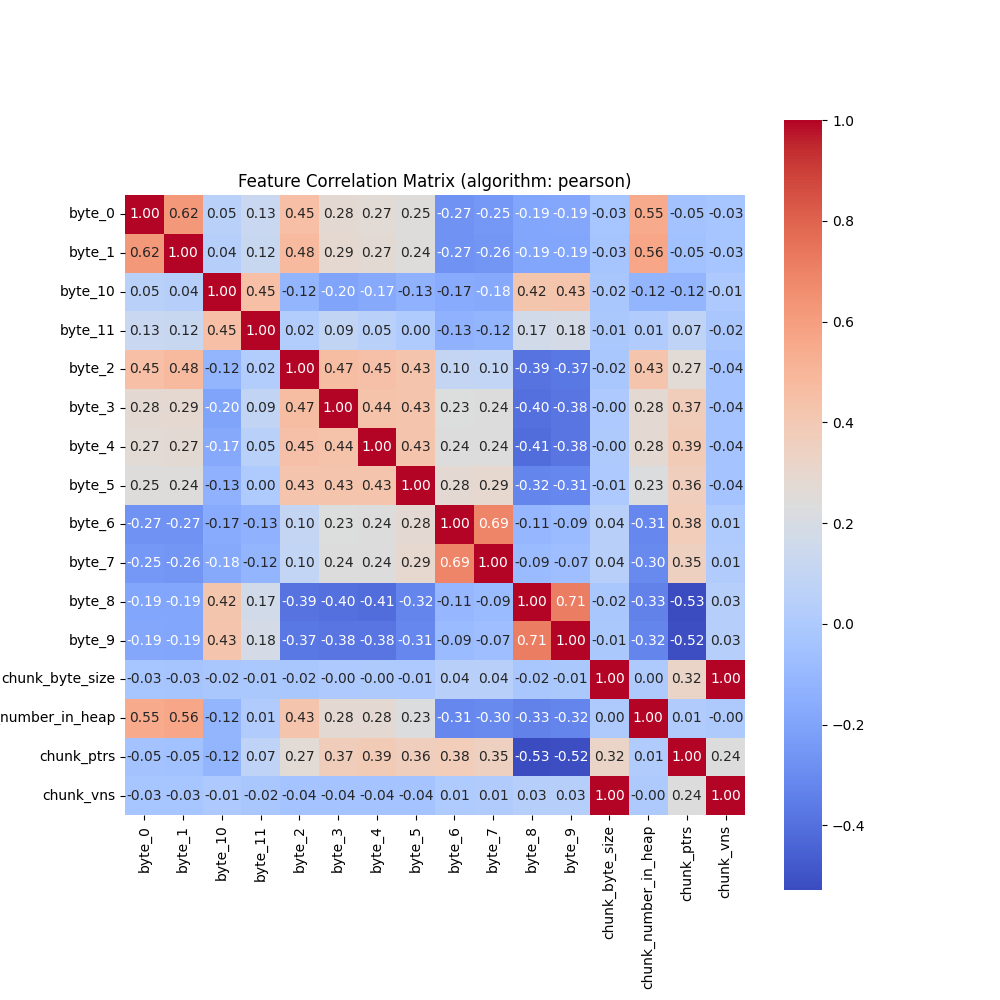
\includegraphics[width=0.8\linewidth]{img/annexes/21/single instance_correlation_matrix.png}} \\
\hline
\end{longtable}


\subsection{22 chunk\_start\_bytes\_embedding (filtered entropy)}

\begin{longtable}{|c|c|}
\caption{single instance Feature Engineering Results on 22} \label{tab:22_single_instance_feature_engineering_results}\\
\hline
Dataset Name & 22 \\ \hline
Instance & single instance \\ \hline
\multirow{8}{*}{Best Features} & chunk\_number\_in\_heap \\ \cline{2-2}
 & chunk\_vns \\ \cline{2-2}
 & chunk\_byte\_size \\ \cline{2-2}
 & byte\_10 \\ \cline{2-2}
 & byte\_1 \\ \cline{2-2}
 & byte\_2 \\ \cline{2-2}
 & byte\_6 \\ \cline{2-2}
 & byte\_11 \\ \cline{2-2}
\noalign{\vskip 5mm}
\multicolumn{2}{|c|}{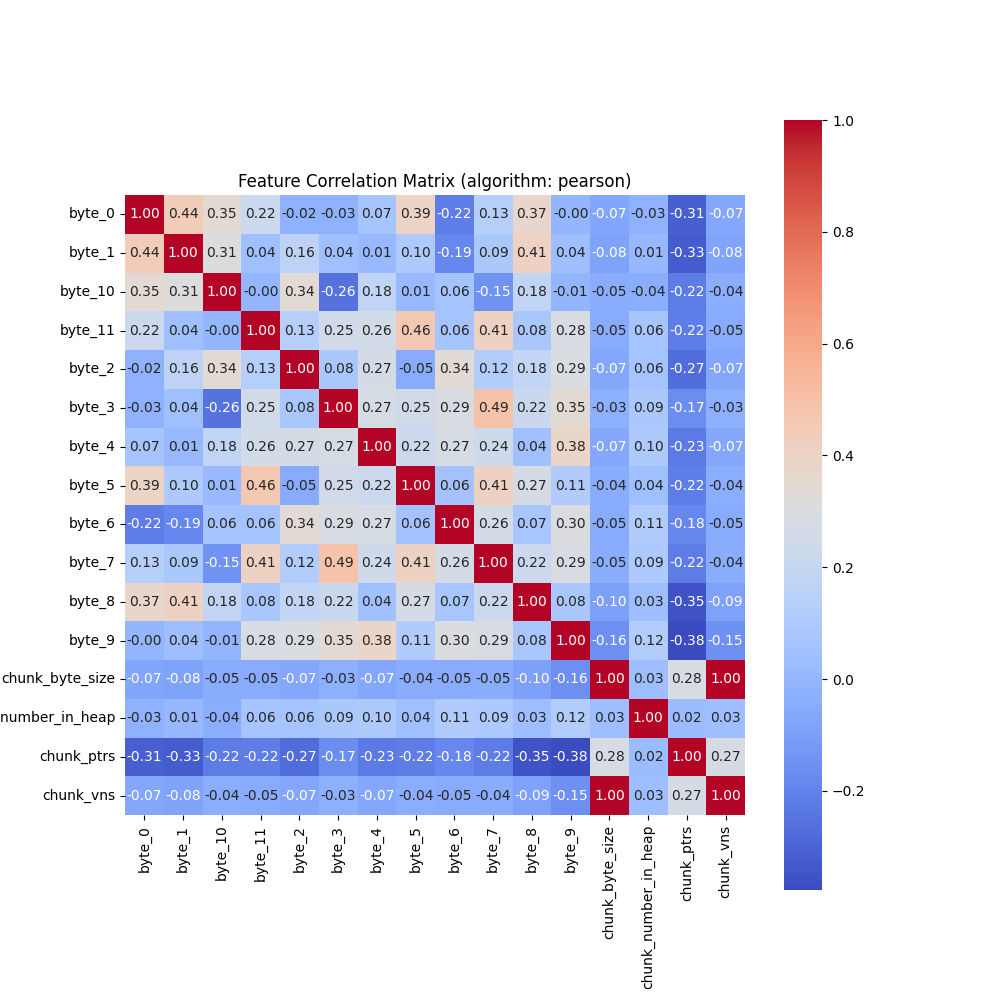
\includegraphics[width=0.8\linewidth]{img/annexes/22/single instance_correlation_matrix.png}} \\
\hline
\end{longtable}


\subsection{23 chunk\_start\_bytes\_embedding (filtered entropy and chunk size)}

\begin{longtable}{|c|c|}
\caption{single instance Feature Engineering Results on 23} \label{tab:23_single_instance_feature_engineering_results}\\
\hline
Dataset Name & 23 \\ \hline
Instance & single instance \\ \hline
\multirow{8}{*}{Best Features} & chunk\_number\_in\_heap \\ \cline{2-2}
 & byte\_2 \\ \cline{2-2}
 & byte\_10 \\ \cline{2-2}
 & byte\_11 \\ \cline{2-2}
 & byte\_6 \\ \cline{2-2}
 & byte\_4 \\ \cline{2-2}
 & byte\_1 \\ \cline{2-2}
 & byte\_8 \\ \cline{2-2}
\noalign{\vskip 5mm}
\multicolumn{2}{|c|}{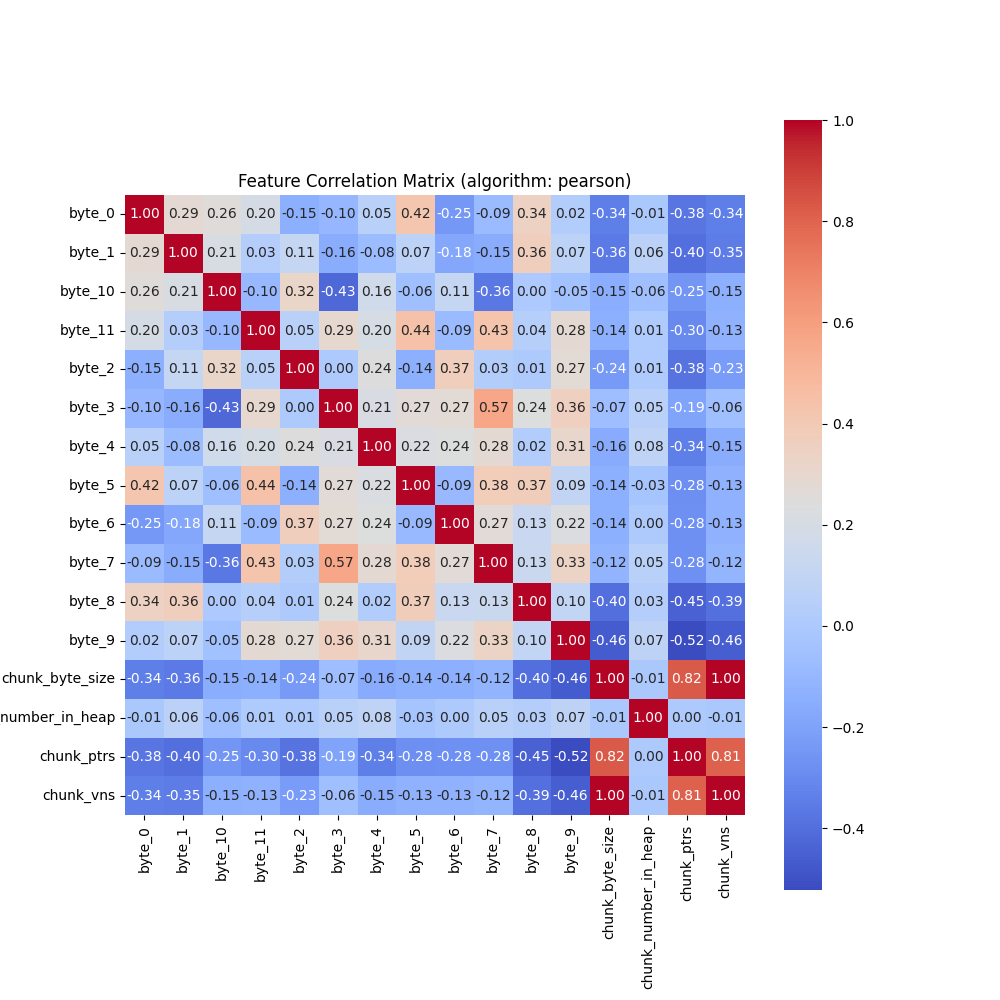
\includegraphics[width=0.8\linewidth]{img/annexes/23/single instance_correlation_matrix.png}} \\
\hline
\end{longtable}


\subsection{25 chunk\_extraction (filtered chunk size)}

\begin{longtable}{|c|c|}
\caption{Word2vec 3 Feature Engineering Results on 25} \label{tab:25_word2vec_3_feature_engineering_results}\\
\hline
Dataset Name & 25 \\ \hline
Instance & Word2vec 3 \\ \hline
\multirow{8}{*}{Best Features} & feature\_2 \\ \cline{2-2}
 & feature\_5 \\ \cline{2-2}
 & feature\_3 \\ \cline{2-2}
 & feature\_6 \\ \cline{2-2}
 & feature\_7 \\ \cline{2-2}
 & feature\_4 \\ \cline{2-2}
 & feature\_0 \\ \cline{2-2}
 & feature\_1 \\ \cline{2-2}
\noalign{\vskip 5mm}
\multicolumn{2}{|c|}{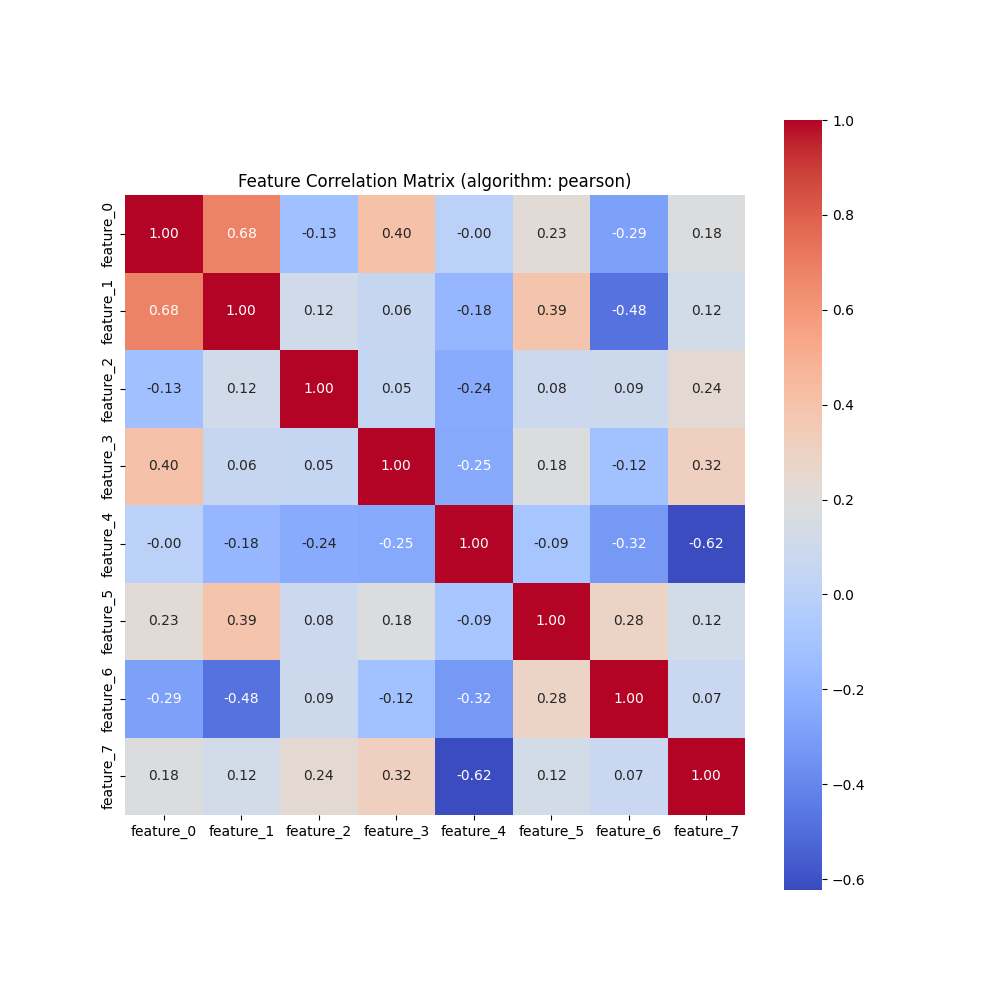
\includegraphics[width=0.8\linewidth]{img/annexes/25/Word2vec 3_correlation_matrix.png}} \\
\hline
\end{longtable}


\subsection{26 chunk\_extraction (filtered entropy)}

\begin{longtable}{|c|c|}
\caption{Transformers 1 Feature Engineering Results on 26} \label{tab:26_transformers_1_feature_engineering_results}\\
\hline
Dataset Name & 26 \\ \hline
Instance & Transformers 1 \\ \hline
\multirow{8}{*}{Best Features} & embedded\_2 \\ \cline{2-2}
 & embedded\_8 \\ \cline{2-2}
 & embedded\_14 \\ \cline{2-2}
 & embedded\_5 \\ \cline{2-2}
 & embedded\_6 \\ \cline{2-2}
 & embedded\_1 \\ \cline{2-2}
 & embedded\_13 \\ \cline{2-2}
 & embedded\_15 \\ \cline{2-2}
\noalign{\vskip 5mm}
\multicolumn{2}{|c|}{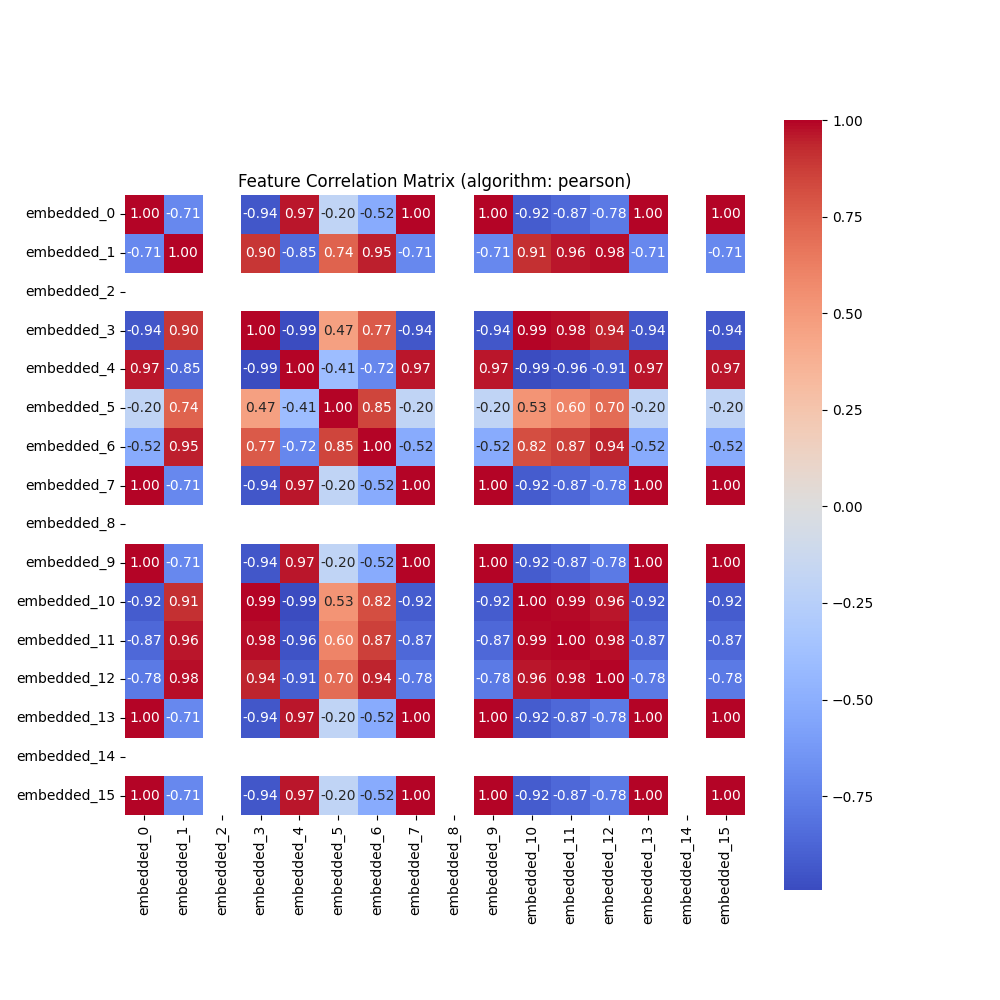
\includegraphics[width=0.8\linewidth]{img/annexes/26/Transformers 1_correlation_matrix.png}} \\
\hline
\end{longtable}


\begin{longtable}{|c|c|}
\caption{Word2vec 1 Feature Engineering Results on 26} \label{tab:26_word2vec_1_feature_engineering_results}\\
\hline
Dataset Name & 26 \\ \hline
Instance & Word2vec 1 \\ \hline
\multirow{8}{*}{Best Features} & feature\_4 \\ \cline{2-2}
 & feature\_5 \\ \cline{2-2}
 & feature\_6 \\ \cline{2-2}
 & feature\_7 \\ \cline{2-2}
 & feature\_2 \\ \cline{2-2}
 & feature\_3 \\ \cline{2-2}
 & feature\_0 \\ \cline{2-2}
 & feature\_1 \\ \cline{2-2}
\noalign{\vskip 5mm}
\multicolumn{2}{|c|}{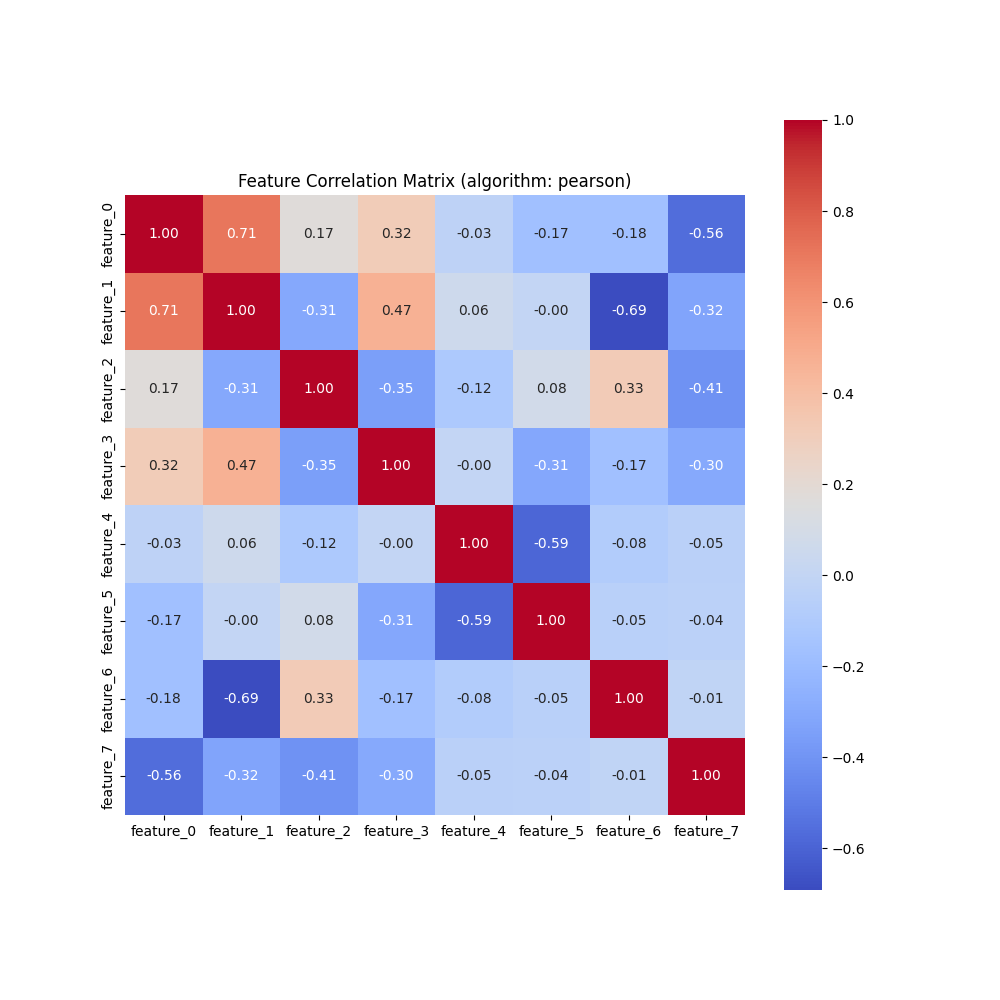
\includegraphics[width=0.8\linewidth]{img/annexes/26/Word2vec 1_correlation_matrix.png}} \\
\hline
\end{longtable}


\subsection{27 chunk\_extraction (filtered entropy and chunk size)}

\begin{longtable}{|c|c|}
\caption{Transformers 1 Feature Engineering Results on 27} \label{tab:27_transformers_1_feature_engineering_results}\\
\hline
Dataset Name & 27 \\ \hline
Instance & Transformers 1 \\ \hline
\multirow{8}{*}{Best Features} & embedded\_0 \\ \cline{2-2}
 & embedded\_6 \\ \cline{2-2}
 & embedded\_7 \\ \cline{2-2}
 & embedded\_9 \\ \cline{2-2}
 & embedded\_8 \\ \cline{2-2}
 & embedded\_10 \\ \cline{2-2}
 & embedded\_5 \\ \cline{2-2}
 & embedded\_3 \\ \cline{2-2}
\noalign{\vskip 5mm}
\multicolumn{2}{|c|}{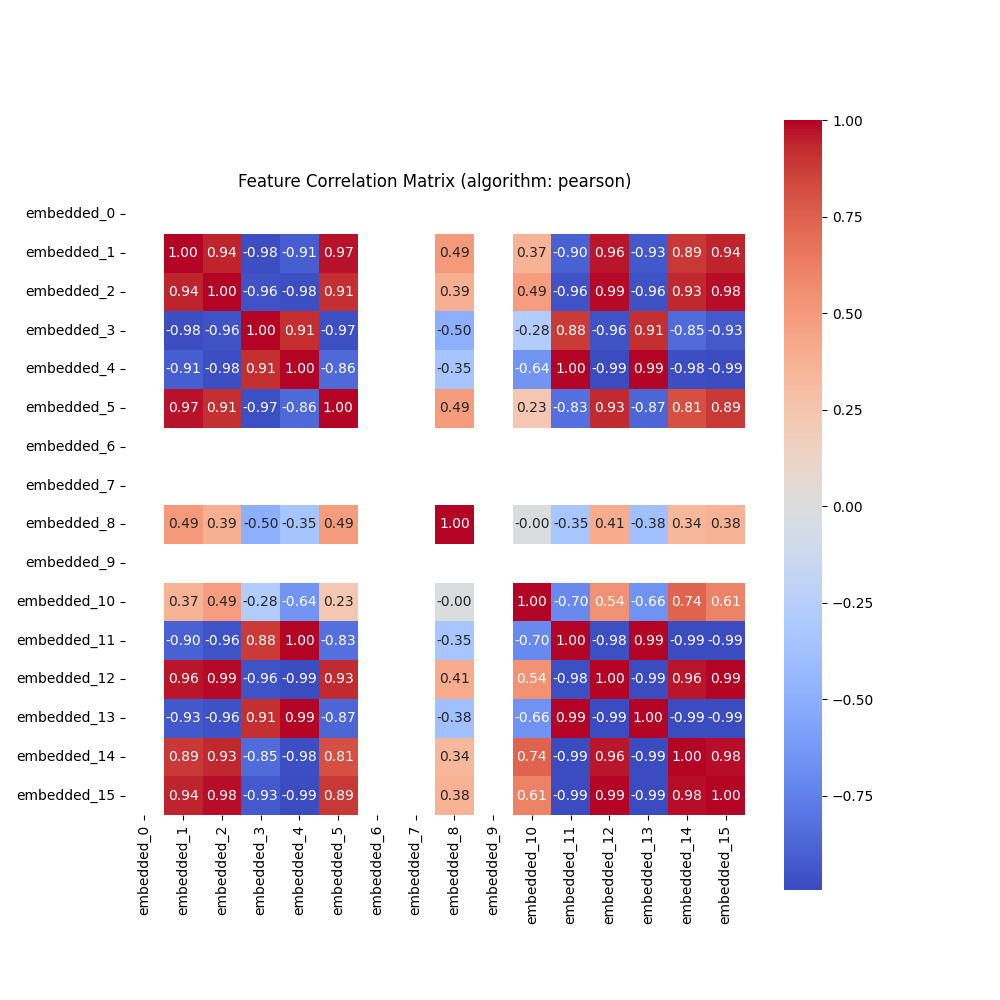
\includegraphics[width=0.8\linewidth]{img/annexes/27/Transformers 1_correlation_matrix.png}} \\
\hline
\end{longtable}


\begin{longtable}{|c|c|}
\caption{Word2vec 3 Feature Engineering Results on 27} \label{tab:27_word2vec_3_feature_engineering_results}\\
\hline
Dataset Name & 27 \\ \hline
Instance & Word2vec 3 \\ \hline
\multirow{8}{*}{Best Features} & feature\_4 \\ \cline{2-2}
 & feature\_3 \\ \cline{2-2}
 & feature\_1 \\ \cline{2-2}
 & feature\_2 \\ \cline{2-2}
 & feature\_0 \\ \cline{2-2}
 & feature\_6 \\ \cline{2-2}
 & feature\_7 \\ \cline{2-2}
 & feature\_5 \\ \cline{2-2}
\noalign{\vskip 5mm}
\multicolumn{2}{|c|}{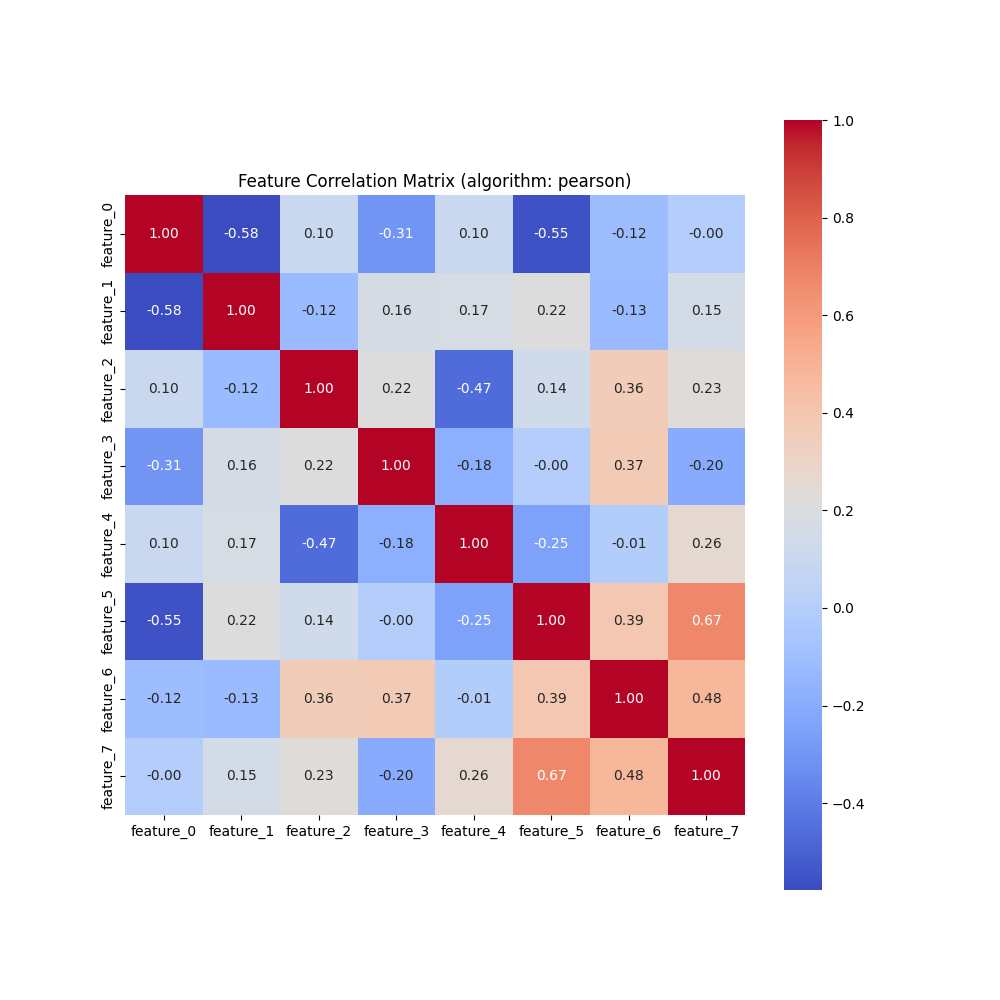
\includegraphics[width=0.8\linewidth]{img/annexes/27/Word2vec 3_correlation_matrix.png}} \\
\hline
\end{longtable}


\section{Clustering results}

\label{sec:annexe:clustering_results}

\subsection{8 chunk\_semantic\_embedding}

\begin{longtable}{|c|c|c|c|c|}
\caption{single instance Clustering Results on 8} \label{tab:8_single_instance_clustering_results}\\
\hline
\multicolumn{5}{|c|}{\textbf{General Information}} \\
\hline
\multicolumn{2}{|c|}{Min Samples} & \multicolumn{3}{c|}{937} \\
\multicolumn{2}{|c|}{Total Duration} & \multicolumn{3}{c|}{3983.122187 s} \\
\hline
\multicolumn{5}{|c|}{\textbf{Clustering Information}} \\
\hline
EPS & Number of Clusters & Silhouette Score & Noise Points & Duration \\
0.01 & 3 & 0.32137176394462585 & 2209 & 795.56207 s\\
0.02 & 3 & 0.12913143634796143 & 3102 & 807.781151 s\\
0.03 & 3 & 0.31343111395835876 & 473 & 808.584517 s\\
0.04 & 3 & 0.30982983112335205 & 484 & 803.3191 s\\
0.05 & 3 & 0.31100085377693176 & 593 & 763.654946 s\\
\hline
\multicolumn{5}{|c|}{\textbf{Best EPS Information}} \\
\hline
0.01 & 3 & 0.32137176394462585 & 2209 & 795.56207 s\\
\hline
\multicolumn{5}{|c|}{\textbf{Label Association}} \\
\hline
Cluster ID & \multicolumn{2}{c|}{Label} & \multicolumn{2}{c|}{Number of Samples} \\
\hline
\multirow{3}{*}{-1.0} & \multicolumn{2}{c|}{1.0} & \multicolumn{2}{c|}{3} \\
& \multicolumn{2}{c|}{2.0} & \multicolumn{2}{c|}{2} \\
& \multicolumn{2}{c|}{4.0} & \multicolumn{2}{c|}{1} \\
\hline
\multirow{4}{*}{0.0} & \multicolumn{2}{c|}{0.0} & \multicolumn{2}{c|}{2} \\
& \multicolumn{2}{c|}{1.0} & \multicolumn{2}{c|}{2} \\
& \multicolumn{2}{c|}{2.0} & \multicolumn{2}{c|}{1} \\
& \multicolumn{2}{c|}{4.0} & \multicolumn{2}{c|}{4} \\
\hline
\multirow{4}{*}{1.0} & \multicolumn{2}{c|}{0.0} & \multicolumn{2}{c|}{1} \\
& \multicolumn{2}{c|}{1.0} & \multicolumn{2}{c|}{5} \\
& \multicolumn{2}{c|}{2.0} & \multicolumn{2}{c|}{1} \\
& \multicolumn{2}{c|}{4.0} & \multicolumn{2}{c|}{1} \\
\hline
\multirow{4}{*}{2.0} & \multicolumn{2}{c|}{0.0} & \multicolumn{2}{c|}{2} \\
& \multicolumn{2}{c|}{1.0} & \multicolumn{2}{c|}{1} \\
& \multicolumn{2}{c|}{2.0} & \multicolumn{2}{c|}{4} \\
& \multicolumn{2}{c|}{4.0} & \multicolumn{2}{c|}{2} \\
\hline
\multicolumn{5}{|c|}{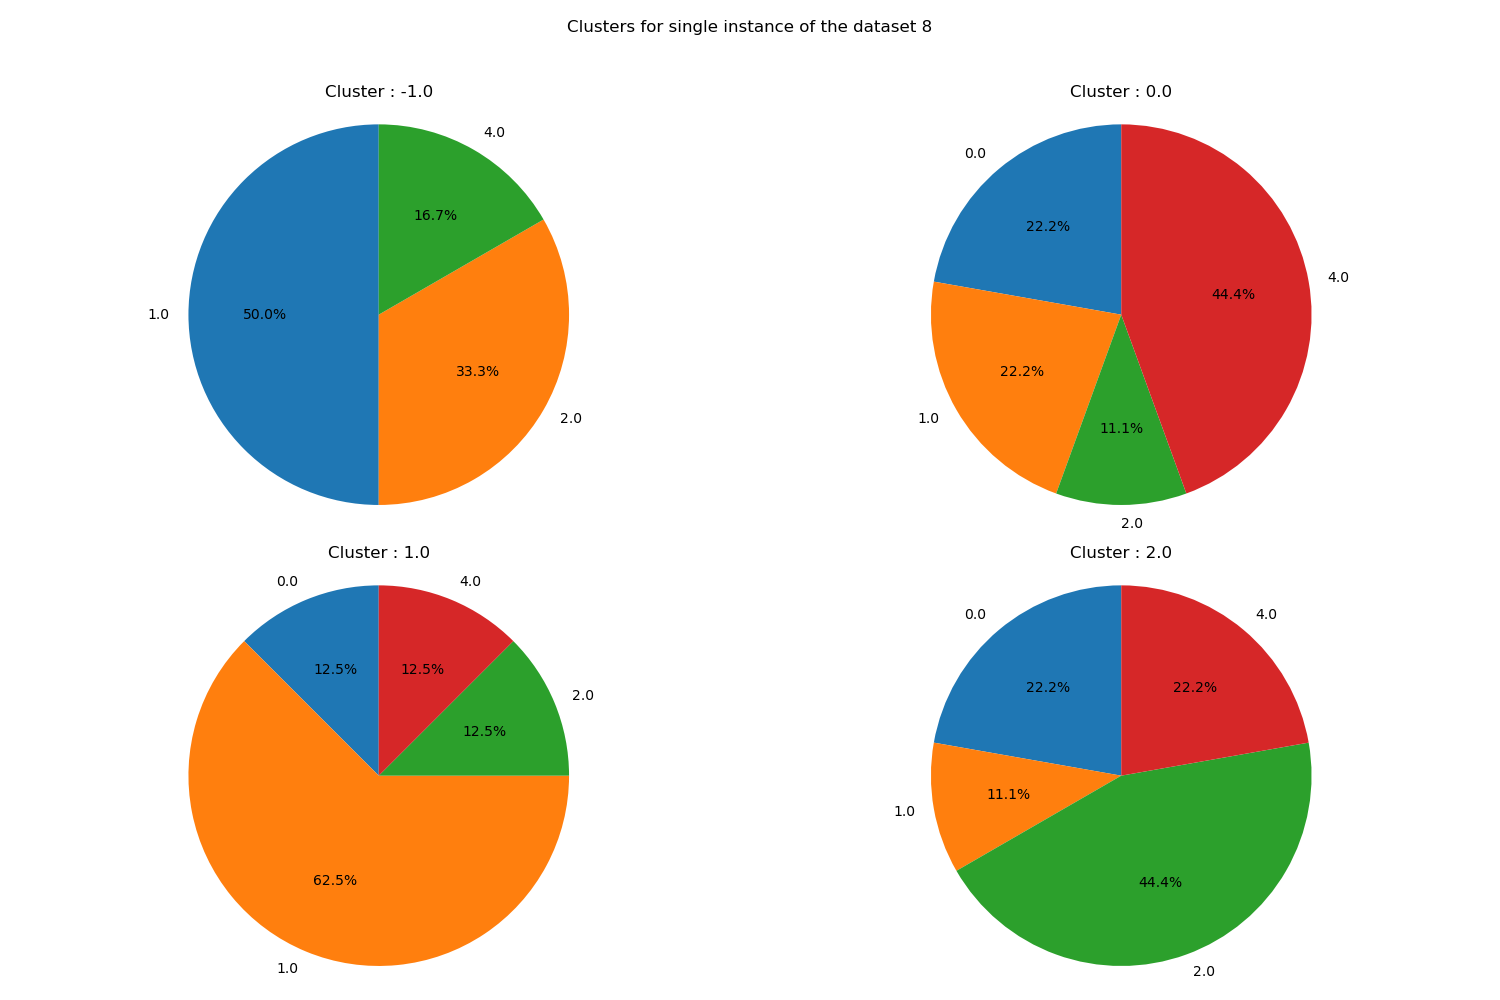
\includegraphics[width=0.8\linewidth]{img/annexes/8/clustering_pie_charts/single instance.png}} \\
\end{longtable}


\subsection{9 chunk\_semantic\_embedding (filtered chunk size)}

\begin{longtable}{|c|c|c|c|c|}
\caption{single instance Clustering Results on 9} \label{tab:9_single_instance_clustering_results}\\
\hline
\multicolumn{5}{|c|}{\textbf{General Information}} \\
\hline
\multicolumn{2}{|c|}{Min Samples} & \multicolumn{3}{c|}{234} \\
\multicolumn{2}{|c|}{Total Duration} & \multicolumn{3}{c|}{3885.123636 s} \\
\hline
\multicolumn{5}{|c|}{\textbf{Clustering Information}} \\
\hline
EPS & Number of Clusters & Silhouette Score & Noise Points & Duration \\
0.01 & 9 & -0.13531261682510376 & 3159 & 790.315211 s\\
0.02 & 9 & -0.14437951147556305 & 3313 & 698.662954 s\\
0.03 & 8 & -0.18256941437721252 & 3907 & 730.104739 s\\
0.04 & 7 & -0.23419693112373352 & 4428 & 786.255948 s\\
0.05 & 7 & -0.2358294278383255 & 4437 & 865.122226 s\\
\hline
\multicolumn{5}{|c|}{\textbf{Best EPS Information}} \\
\hline
0.01 & 9 & -0.13531261682510376 & 3159 & 790.315211 s\\
\hline
\multicolumn{5}{|c|}{\textbf{Label Association}} \\
\hline
Cluster ID & \multicolumn{2}{c|}{Label} & \multicolumn{2}{c|}{Number of Samples} \\
\hline
\multirow{4}{*}{-1.0} & \multicolumn{2}{c|}{0.0} & \multicolumn{2}{c|}{3122} \\
& \multicolumn{2}{c|}{1.0} & \multicolumn{2}{c|}{26} \\
& \multicolumn{2}{c|}{2.0} & \multicolumn{2}{c|}{7} \\
& \multicolumn{2}{c|}{4.0} & \multicolumn{2}{c|}{4} \\
\hline
\multirow{2}{*}{0.0} & \multicolumn{2}{c|}{0.0} & \multicolumn{2}{c|}{550} \\
& \multicolumn{2}{c|}{1.0} & \multicolumn{2}{c|}{4} \\
\hline
\multirow{3}{*}{1.0} & \multicolumn{2}{c|}{0.0} & \multicolumn{2}{c|}{302} \\
& \multicolumn{2}{c|}{1.0} & \multicolumn{2}{c|}{4} \\
& \multicolumn{2}{c|}{4.0} & \multicolumn{2}{c|}{2} \\
\hline
\multirow{3}{*}{2.0} & \multicolumn{2}{c|}{0.0} & \multicolumn{2}{c|}{424} \\
& \multicolumn{2}{c|}{1.0} & \multicolumn{2}{c|}{2} \\
& \multicolumn{2}{c|}{4.0} & \multicolumn{2}{c|}{1} \\
\hline
\multirow{4}{*}{3.0} & \multicolumn{2}{c|}{0.0} & \multicolumn{2}{c|}{422} \\
& \multicolumn{2}{c|}{1.0} & \multicolumn{2}{c|}{4} \\
& \multicolumn{2}{c|}{2.0} & \multicolumn{2}{c|}{1} \\
& \multicolumn{2}{c|}{4.0} & \multicolumn{2}{c|}{1} \\
\hline
\multirow{2}{*}{4.0} & \multicolumn{2}{c|}{0.0} & \multicolumn{2}{c|}{665} \\
& \multicolumn{2}{c|}{1.0} & \multicolumn{2}{c|}{4} \\
\hline
\multirow{4}{*}{5.0} & \multicolumn{2}{c|}{0.0} & \multicolumn{2}{c|}{448} \\
& \multicolumn{2}{c|}{1.0} & \multicolumn{2}{c|}{6} \\
& \multicolumn{2}{c|}{2.0} & \multicolumn{2}{c|}{1} \\
& \multicolumn{2}{c|}{4.0} & \multicolumn{2}{c|}{1} \\
\hline
\multirow{2}{*}{6.0} & \multicolumn{2}{c|}{0.0} & \multicolumn{2}{c|}{505} \\
& \multicolumn{2}{c|}{1.0} & \multicolumn{2}{c|}{4} \\
\hline
\multirow{4}{*}{7.0} & \multicolumn{2}{c|}{0.0} & \multicolumn{2}{c|}{403} \\
& \multicolumn{2}{c|}{1.0} & \multicolumn{2}{c|}{2} \\
& \multicolumn{2}{c|}{2.0} & \multicolumn{2}{c|}{1} \\
& \multicolumn{2}{c|}{4.0} & \multicolumn{2}{c|}{1} \\
\hline
\multirow{2}{*}{8.0} & \multicolumn{2}{c|}{0.0} & \multicolumn{2}{c|}{577} \\
& \multicolumn{2}{c|}{1.0} & \multicolumn{2}{c|}{4} \\
\hline
\multicolumn{5}{|c|}{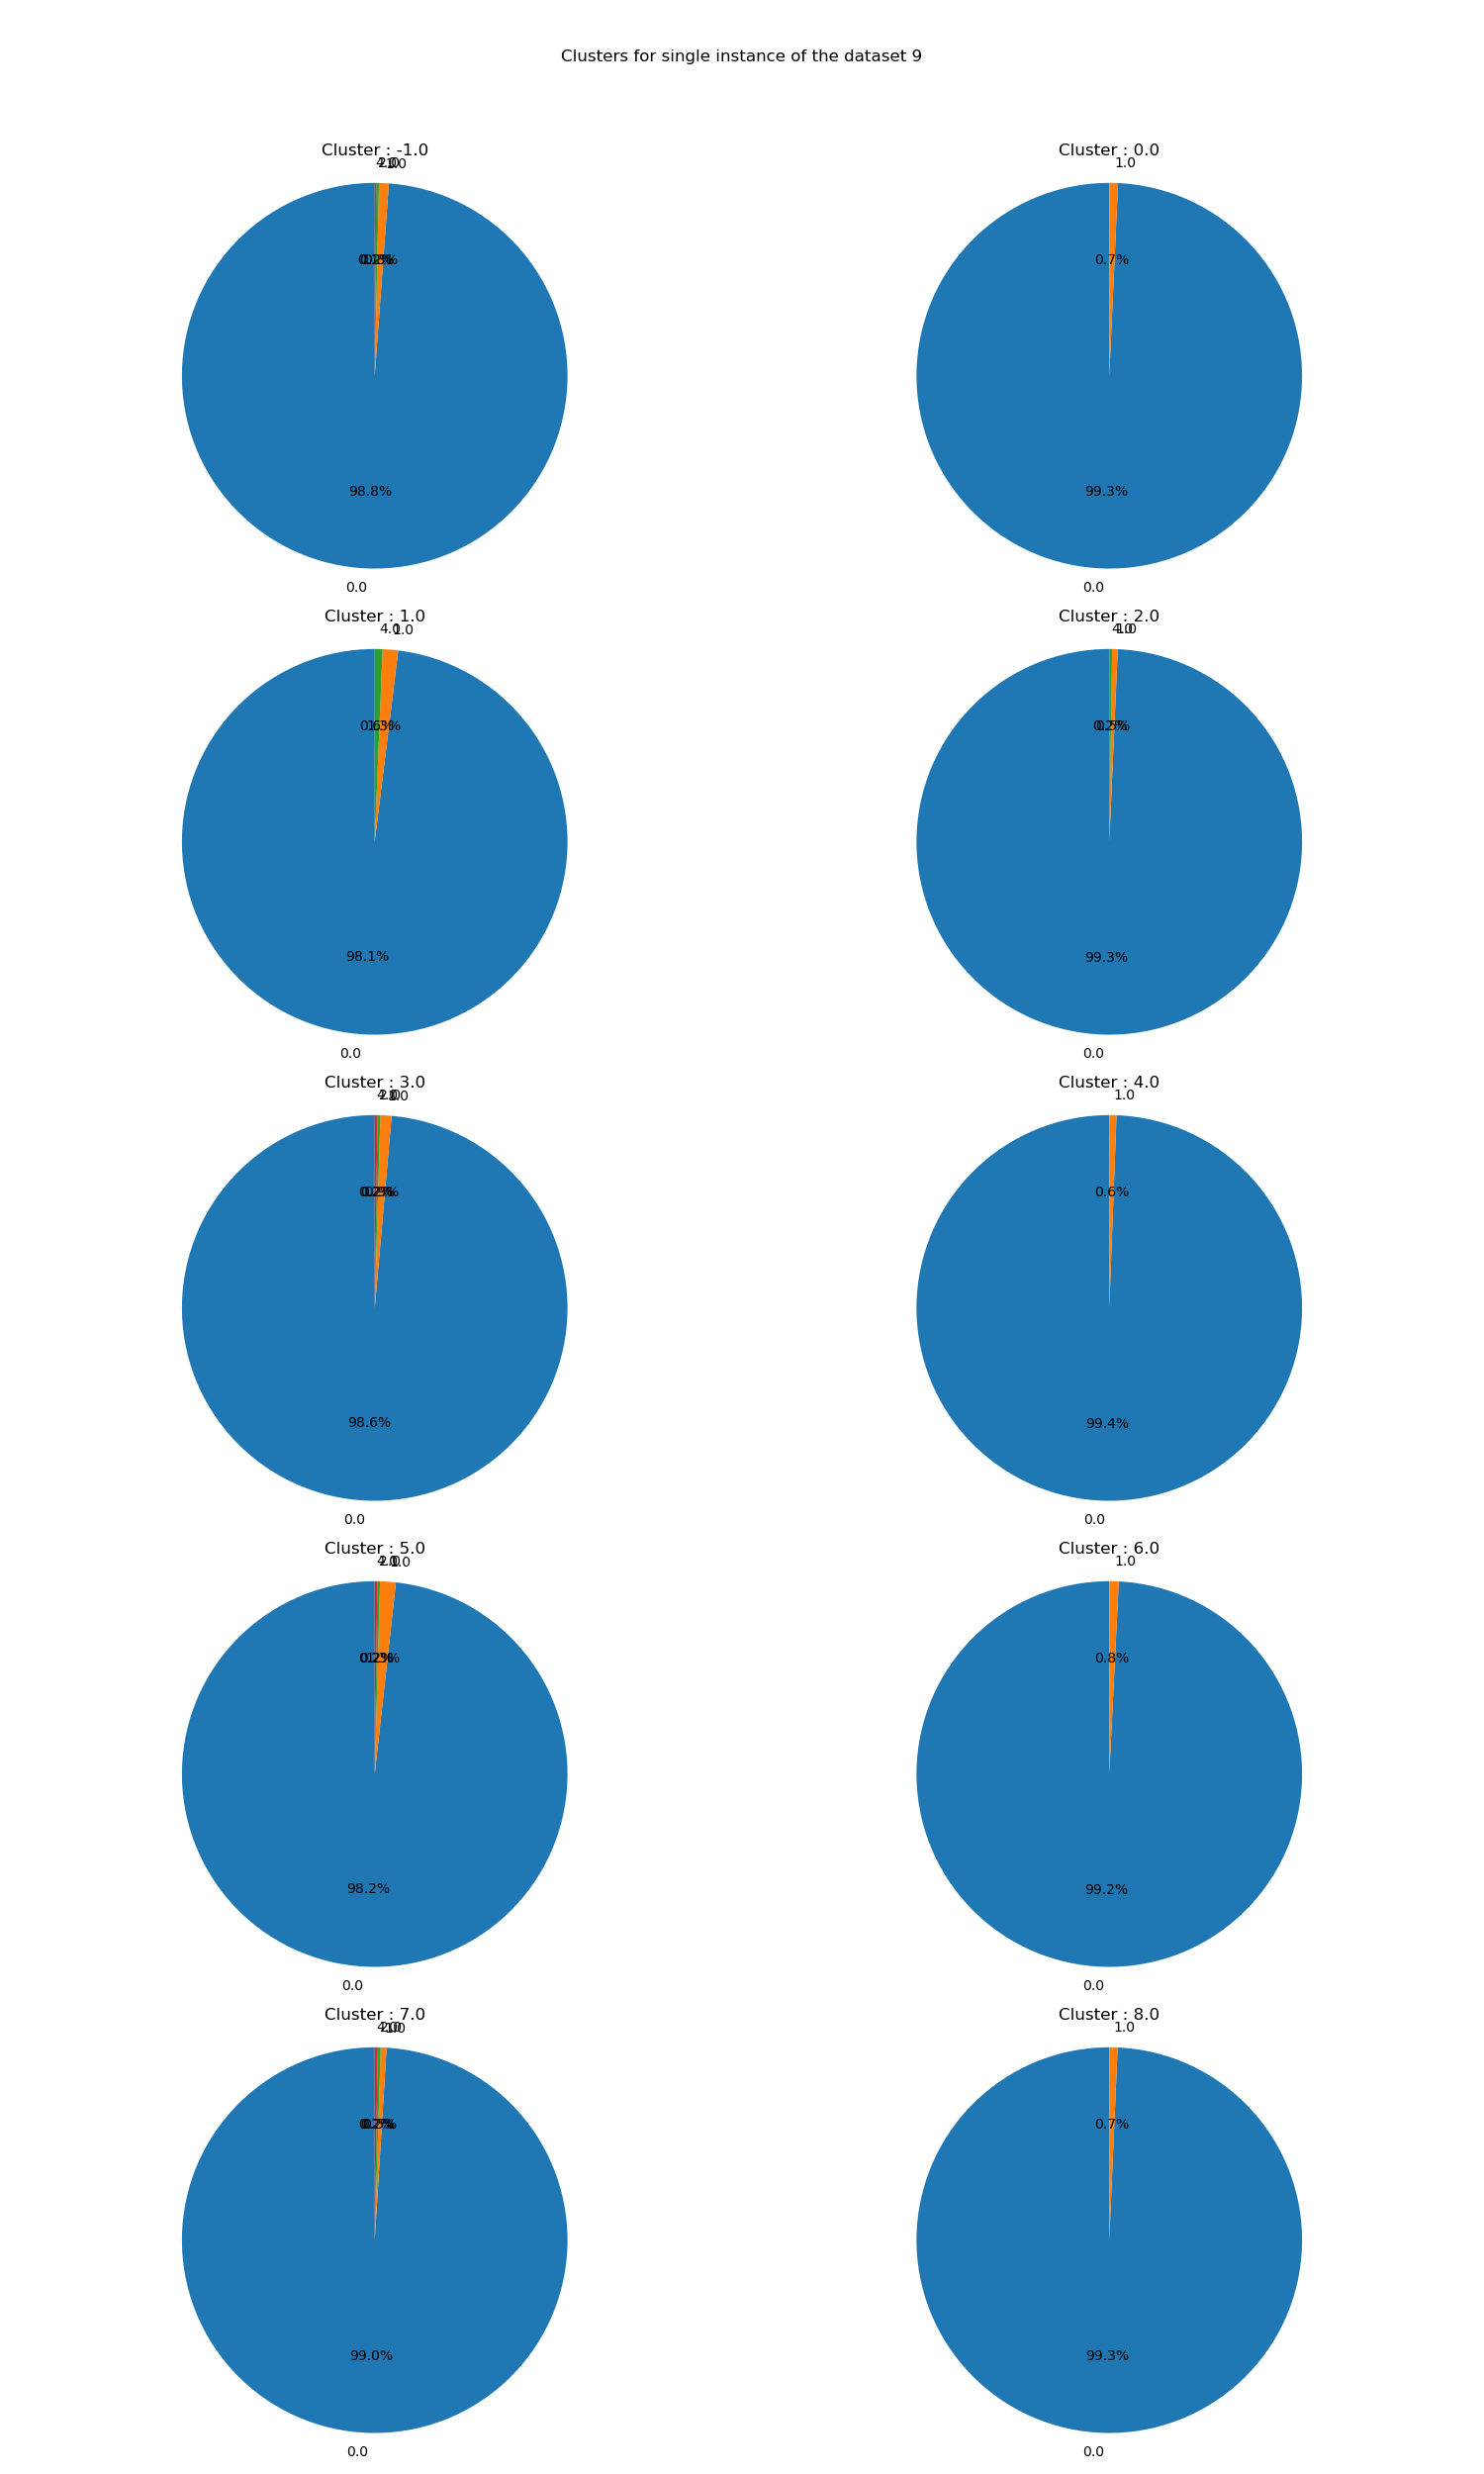
\includegraphics[width=0.8\linewidth]{img/annexes/9/clustering_pie_charts/single instance.png}} \\
\end{longtable}


\subsection{10 chunk\_semantic\_embedding (filtered entropy)}

\begin{longtable}{|c|c|c|c|c|}
\caption{single instance Clustering Results on 10} \label{tab:10_single_instance_clustering_results}\\
\hline
\multicolumn{5}{|c|}{\textbf{General Information}} \\
\hline
\multicolumn{2}{|c|}{Min Samples} & \multicolumn{3}{c|}{234} \\
\multicolumn{2}{|c|}{Total Duration} & \multicolumn{3}{c|}{4226.531537 s} \\
\hline
\multicolumn{5}{|c|}{\textbf{Clustering Information}} \\
\hline
EPS & Number of Clusters & Silhouette Score & Noise Points & Duration \\
0.01 & 13 & -0.12140722572803497 & 2271 & 839.513428 s\\
0.02 & 13 & -0.12140722572803497 & 2271 & 871.127049 s\\
0.03 & 13 & -0.12140722572803497 & 2271 & 923.602916 s\\
0.04 & 13 & -0.12195669114589691 & 2276 & 857.46417 s\\
0.05 & 13 & -0.049609262496232986 & 1886 & 730.73765 s\\
\hline
\multicolumn{5}{|c|}{\textbf{Best EPS Information}} \\
\hline
0.05 & 13 & -0.049609262496232986 & 1886 & 730.73765 s\\
\hline
\multicolumn{5}{|c|}{\textbf{Label Association}} \\
\hline
Cluster ID & \multicolumn{2}{c|}{Label} & \multicolumn{2}{c|}{Number of Samples} \\
\hline
\multirow{4}{*}{-1.0} & \multicolumn{2}{c|}{0.0} & \multicolumn{2}{c|}{1488} \\
& \multicolumn{2}{c|}{1.0} & \multicolumn{2}{c|}{296} \\
& \multicolumn{2}{c|}{2.0} & \multicolumn{2}{c|}{48} \\
& \multicolumn{2}{c|}{4.0} & \multicolumn{2}{c|}{54} \\
\hline
\multirow{4}{*}{0.0} & \multicolumn{2}{c|}{0.0} & \multicolumn{2}{c|}{353} \\
& \multicolumn{2}{c|}{1.0} & \multicolumn{2}{c|}{71} \\
& \multicolumn{2}{c|}{2.0} & \multicolumn{2}{c|}{14} \\
& \multicolumn{2}{c|}{4.0} & \multicolumn{2}{c|}{7} \\
\hline
\multirow{4}{*}{1.0} & \multicolumn{2}{c|}{0.0} & \multicolumn{2}{c|}{502} \\
& \multicolumn{2}{c|}{1.0} & \multicolumn{2}{c|}{111} \\
& \multicolumn{2}{c|}{2.0} & \multicolumn{2}{c|}{16} \\
& \multicolumn{2}{c|}{4.0} & \multicolumn{2}{c|}{14} \\
\hline
\multirow{4}{*}{2.0} & \multicolumn{2}{c|}{0.0} & \multicolumn{2}{c|}{201} \\
& \multicolumn{2}{c|}{1.0} & \multicolumn{2}{c|}{24} \\
& \multicolumn{2}{c|}{2.0} & \multicolumn{2}{c|}{8} \\
& \multicolumn{2}{c|}{4.0} & \multicolumn{2}{c|}{4} \\
\hline
\multirow{4}{*}{3.0} & \multicolumn{2}{c|}{0.0} & \multicolumn{2}{c|}{259} \\
& \multicolumn{2}{c|}{1.0} & \multicolumn{2}{c|}{63} \\
& \multicolumn{2}{c|}{2.0} & \multicolumn{2}{c|}{10} \\
& \multicolumn{2}{c|}{4.0} & \multicolumn{2}{c|}{12} \\
\hline
\multirow{4}{*}{4.0} & \multicolumn{2}{c|}{0.0} & \multicolumn{2}{c|}{343} \\
& \multicolumn{2}{c|}{1.0} & \multicolumn{2}{c|}{68} \\
& \multicolumn{2}{c|}{2.0} & \multicolumn{2}{c|}{14} \\
& \multicolumn{2}{c|}{4.0} & \multicolumn{2}{c|}{16} \\
\hline
\multirow{4}{*}{5.0} & \multicolumn{2}{c|}{0.0} & \multicolumn{2}{c|}{320} \\
& \multicolumn{2}{c|}{1.0} & \multicolumn{2}{c|}{64} \\
& \multicolumn{2}{c|}{2.0} & \multicolumn{2}{c|}{17} \\
& \multicolumn{2}{c|}{4.0} & \multicolumn{2}{c|}{13} \\
\hline
\multirow{4}{*}{6.0} & \multicolumn{2}{c|}{0.0} & \multicolumn{2}{c|}{458} \\
& \multicolumn{2}{c|}{1.0} & \multicolumn{2}{c|}{92} \\
& \multicolumn{2}{c|}{2.0} & \multicolumn{2}{c|}{12} \\
& \multicolumn{2}{c|}{4.0} & \multicolumn{2}{c|}{16} \\
\hline
\multirow{4}{*}{7.0} & \multicolumn{2}{c|}{0.0} & \multicolumn{2}{c|}{383} \\
& \multicolumn{2}{c|}{1.0} & \multicolumn{2}{c|}{81} \\
& \multicolumn{2}{c|}{2.0} & \multicolumn{2}{c|}{8} \\
& \multicolumn{2}{c|}{4.0} & \multicolumn{2}{c|}{15} \\
\hline
\multirow{4}{*}{8.0} & \multicolumn{2}{c|}{0.0} & \multicolumn{2}{c|}{276} \\
& \multicolumn{2}{c|}{1.0} & \multicolumn{2}{c|}{70} \\
& \multicolumn{2}{c|}{2.0} & \multicolumn{2}{c|}{5} \\
& \multicolumn{2}{c|}{4.0} & \multicolumn{2}{c|}{7} \\
\hline
\multirow{4}{*}{9.0} & \multicolumn{2}{c|}{0.0} & \multicolumn{2}{c|}{617} \\
& \multicolumn{2}{c|}{1.0} & \multicolumn{2}{c|}{119} \\
& \multicolumn{2}{c|}{2.0} & \multicolumn{2}{c|}{23} \\
& \multicolumn{2}{c|}{4.0} & \multicolumn{2}{c|}{21} \\
\hline
\multirow{4}{*}{10.0} & \multicolumn{2}{c|}{0.0} & \multicolumn{2}{c|}{233} \\
& \multicolumn{2}{c|}{1.0} & \multicolumn{2}{c|}{45} \\
& \multicolumn{2}{c|}{2.0} & \multicolumn{2}{c|}{9} \\
& \multicolumn{2}{c|}{4.0} & \multicolumn{2}{c|}{9} \\
\hline
\multirow{4}{*}{11.0} & \multicolumn{2}{c|}{0.0} & \multicolumn{2}{c|}{196} \\
& \multicolumn{2}{c|}{1.0} & \multicolumn{2}{c|}{33} \\
& \multicolumn{2}{c|}{2.0} & \multicolumn{2}{c|}{6} \\
& \multicolumn{2}{c|}{4.0} & \multicolumn{2}{c|}{3} \\
\hline
\multirow{4}{*}{12.0} & \multicolumn{2}{c|}{0.0} & \multicolumn{2}{c|}{272} \\
& \multicolumn{2}{c|}{1.0} & \multicolumn{2}{c|}{60} \\
& \multicolumn{2}{c|}{2.0} & \multicolumn{2}{c|}{10} \\
& \multicolumn{2}{c|}{4.0} & \multicolumn{2}{c|}{9} \\
\hline
\multicolumn{5}{|c|}{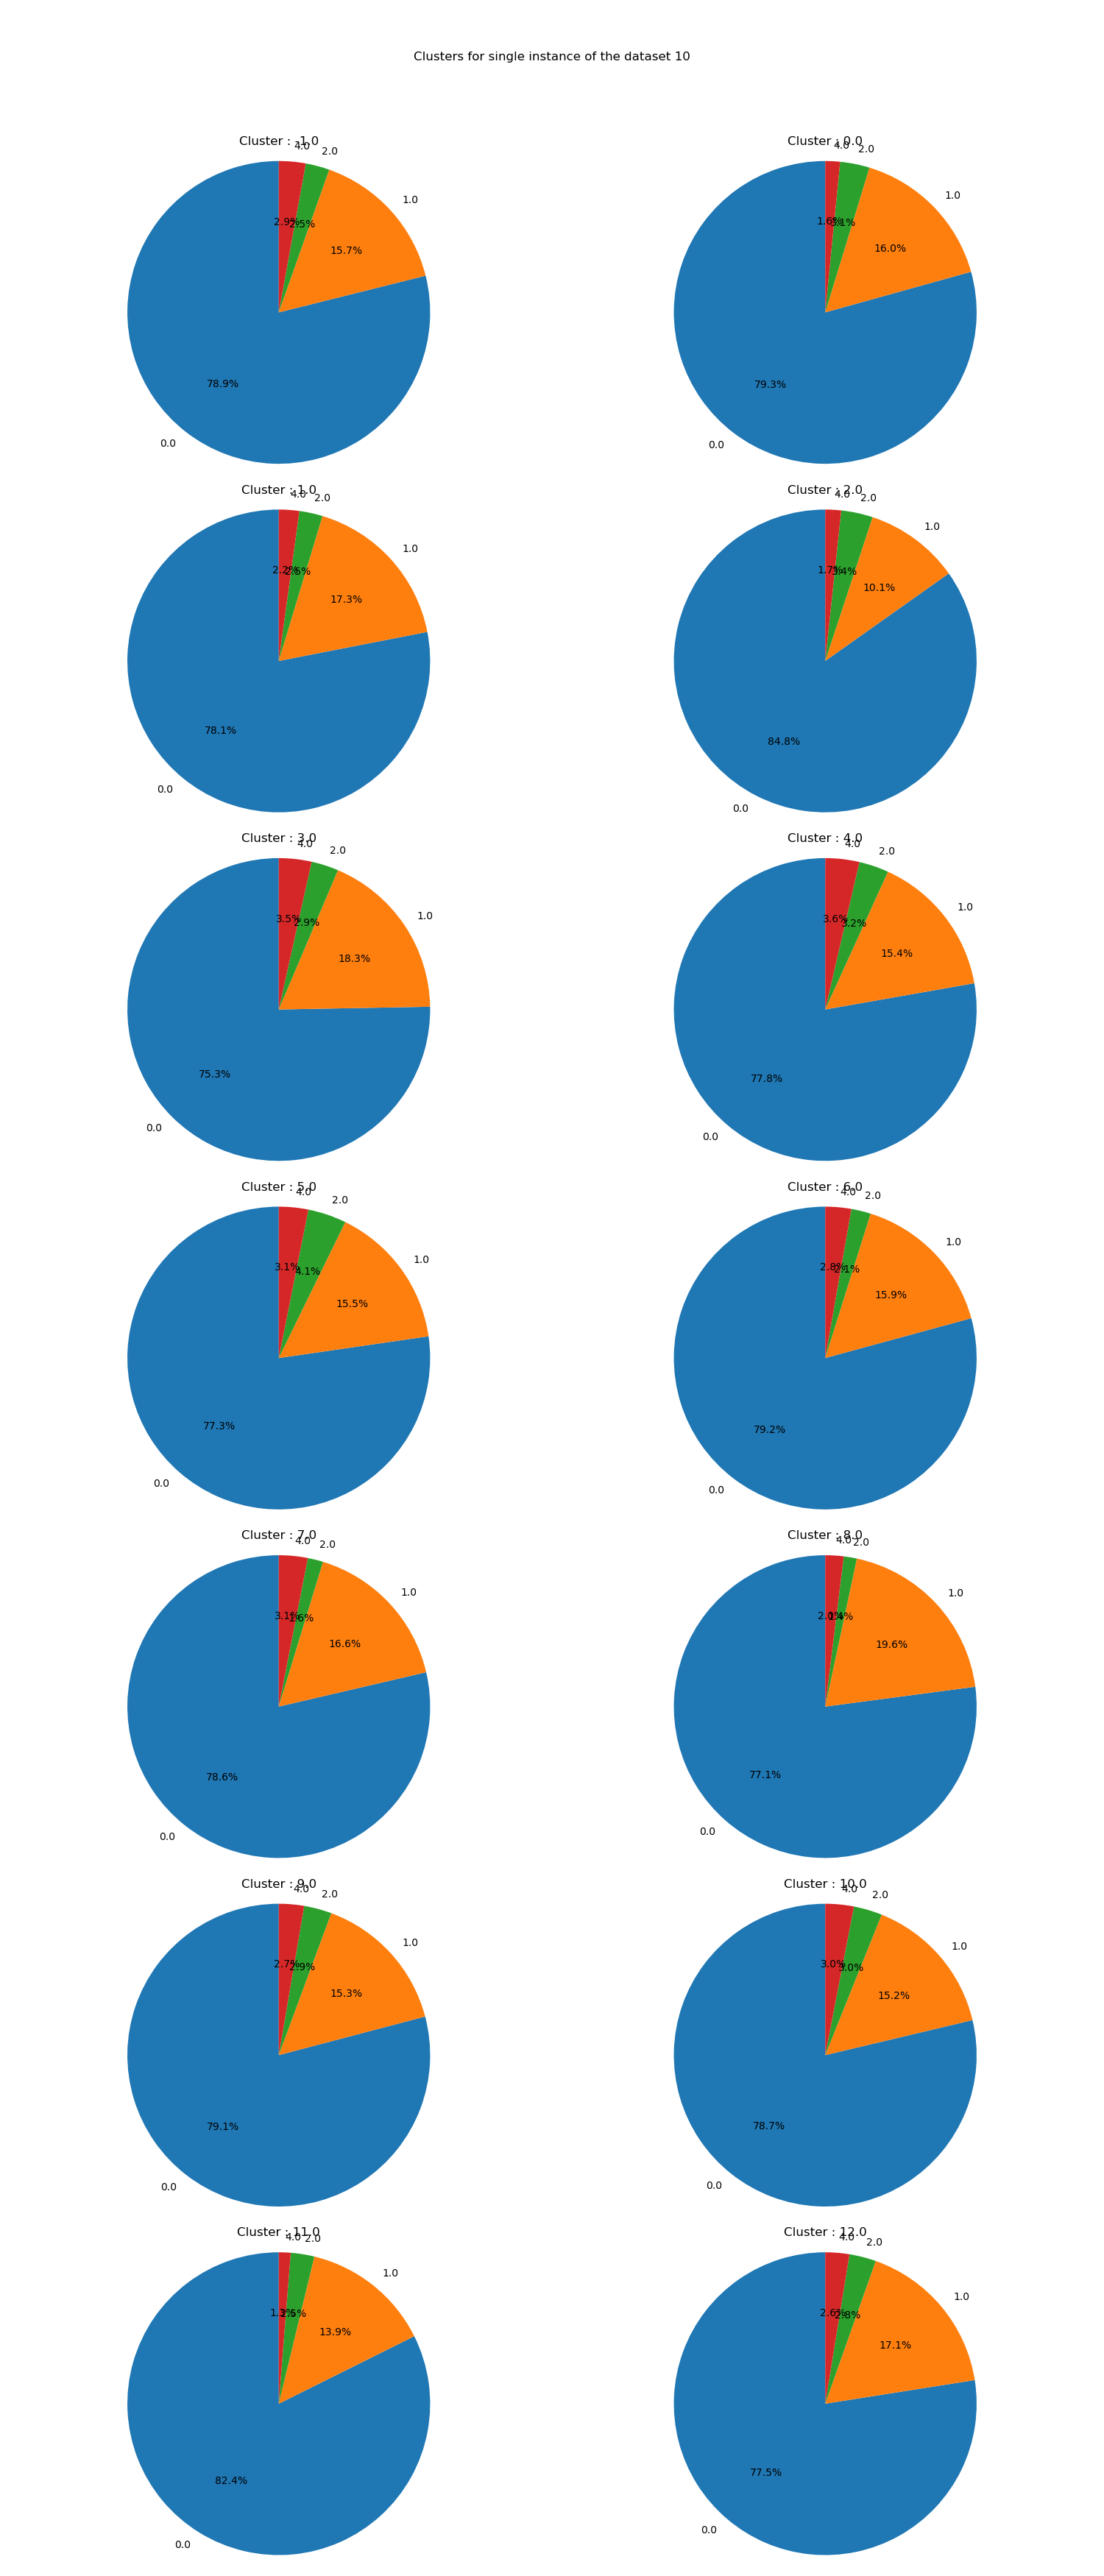
\includegraphics[width=0.8\linewidth]{img/annexes/10/clustering_pie_charts/single instance.png}} \\
\end{longtable}


\subsection{11 chunk\_semantic\_embedding (filtered entropy and chunk size)}

\begin{longtable}{|c|c|c|c|c|}
\caption{single instance Clustering Results on 11} \label{tab:11_single_instance_clustering_results}\\
\hline
\multicolumn{5}{|c|}{\textbf{General Information}} \\
\hline
\multicolumn{2}{|c|}{Min Samples} & \multicolumn{3}{c|}{234} \\
\multicolumn{2}{|c|}{Total Duration} & \multicolumn{3}{c|}{3952.659099 s} \\
\hline
\multicolumn{5}{|c|}{\textbf{Clustering Information}} \\
\hline
EPS & Number of Clusters & Silhouette Score & Noise Points & Duration \\
0.01 & 10 & -0.3094848692417145 & 3931 & 916.861663 s\\
0.02 & 10 & -0.21667371690273285 & 3518 & 758.388542 s\\
0.03 & 10 & -0.22114033997058868 & 3554 & 724.996902 s\\
0.04 & 10 & -0.22928959131240845 & 3594 & 767.8521 s\\
0.05 & 10 & -0.2298821657896042 & 3601 & 779.975939 s\\
\hline
\multicolumn{5}{|c|}{\textbf{Best EPS Information}} \\
\hline
0.02 & 10 & -0.21667371690273285 & 3518 & 758.388542 s\\
\hline
\multicolumn{5}{|c|}{\textbf{Label Association}} \\
\hline
Cluster ID & \multicolumn{2}{c|}{Label} & \multicolumn{2}{c|}{Number of Samples} \\
\hline
\multirow{4}{*}{-1.0} & \multicolumn{2}{c|}{0.0} & \multicolumn{2}{c|}{2431} \\
& \multicolumn{2}{c|}{1.0} & \multicolumn{2}{c|}{817} \\
& \multicolumn{2}{c|}{2.0} & \multicolumn{2}{c|}{132} \\
& \multicolumn{2}{c|}{4.0} & \multicolumn{2}{c|}{138} \\
\hline
\multirow{4}{*}{0.0} & \multicolumn{2}{c|}{0.0} & \multicolumn{2}{c|}{164} \\
& \multicolumn{2}{c|}{1.0} & \multicolumn{2}{c|}{52} \\
& \multicolumn{2}{c|}{2.0} & \multicolumn{2}{c|}{13} \\
& \multicolumn{2}{c|}{4.0} & \multicolumn{2}{c|}{14} \\
\hline
\multirow{4}{*}{1.0} & \multicolumn{2}{c|}{0.0} & \multicolumn{2}{c|}{452} \\
& \multicolumn{2}{c|}{1.0} & \multicolumn{2}{c|}{146} \\
& \multicolumn{2}{c|}{2.0} & \multicolumn{2}{c|}{21} \\
& \multicolumn{2}{c|}{4.0} & \multicolumn{2}{c|}{18} \\
\hline
\multirow{4}{*}{2.0} & \multicolumn{2}{c|}{0.0} & \multicolumn{2}{c|}{471} \\
& \multicolumn{2}{c|}{1.0} & \multicolumn{2}{c|}{162} \\
& \multicolumn{2}{c|}{2.0} & \multicolumn{2}{c|}{22} \\
& \multicolumn{2}{c|}{4.0} & \multicolumn{2}{c|}{28} \\
\hline
\multirow{4}{*}{3.0} & \multicolumn{2}{c|}{0.0} & \multicolumn{2}{c|}{187} \\
& \multicolumn{2}{c|}{1.0} & \multicolumn{2}{c|}{60} \\
& \multicolumn{2}{c|}{2.0} & \multicolumn{2}{c|}{15} \\
& \multicolumn{2}{c|}{4.0} & \multicolumn{2}{c|}{9} \\
\hline
\multirow{4}{*}{4.0} & \multicolumn{2}{c|}{0.0} & \multicolumn{2}{c|}{207} \\
& \multicolumn{2}{c|}{1.0} & \multicolumn{2}{c|}{61} \\
& \multicolumn{2}{c|}{2.0} & \multicolumn{2}{c|}{8} \\
& \multicolumn{2}{c|}{4.0} & \multicolumn{2}{c|}{10} \\
\hline
\multirow{4}{*}{5.0} & \multicolumn{2}{c|}{0.0} & \multicolumn{2}{c|}{221} \\
& \multicolumn{2}{c|}{1.0} & \multicolumn{2}{c|}{66} \\
& \multicolumn{2}{c|}{2.0} & \multicolumn{2}{c|}{12} \\
& \multicolumn{2}{c|}{4.0} & \multicolumn{2}{c|}{12} \\
\hline
\multirow{4}{*}{6.0} & \multicolumn{2}{c|}{0.0} & \multicolumn{2}{c|}{202} \\
& \multicolumn{2}{c|}{1.0} & \multicolumn{2}{c|}{50} \\
& \multicolumn{2}{c|}{2.0} & \multicolumn{2}{c|}{6} \\
& \multicolumn{2}{c|}{4.0} & \multicolumn{2}{c|}{7} \\
\hline
\multirow{4}{*}{7.0} & \multicolumn{2}{c|}{0.0} & \multicolumn{2}{c|}{202} \\
& \multicolumn{2}{c|}{1.0} & \multicolumn{2}{c|}{76} \\
& \multicolumn{2}{c|}{2.0} & \multicolumn{2}{c|}{17} \\
& \multicolumn{2}{c|}{4.0} & \multicolumn{2}{c|}{10} \\
\hline
\multirow{4}{*}{8.0} & \multicolumn{2}{c|}{0.0} & \multicolumn{2}{c|}{223} \\
& \multicolumn{2}{c|}{1.0} & \multicolumn{2}{c|}{91} \\
& \multicolumn{2}{c|}{2.0} & \multicolumn{2}{c|}{19} \\
& \multicolumn{2}{c|}{4.0} & \multicolumn{2}{c|}{11} \\
\hline
\multirow{4}{*}{9.0} & \multicolumn{2}{c|}{0.0} & \multicolumn{2}{c|}{437} \\
& \multicolumn{2}{c|}{1.0} & \multicolumn{2}{c|}{146} \\
& \multicolumn{2}{c|}{2.0} & \multicolumn{2}{c|}{22} \\
& \multicolumn{2}{c|}{4.0} & \multicolumn{2}{c|}{30} \\
\hline
\multicolumn{5}{|c|}{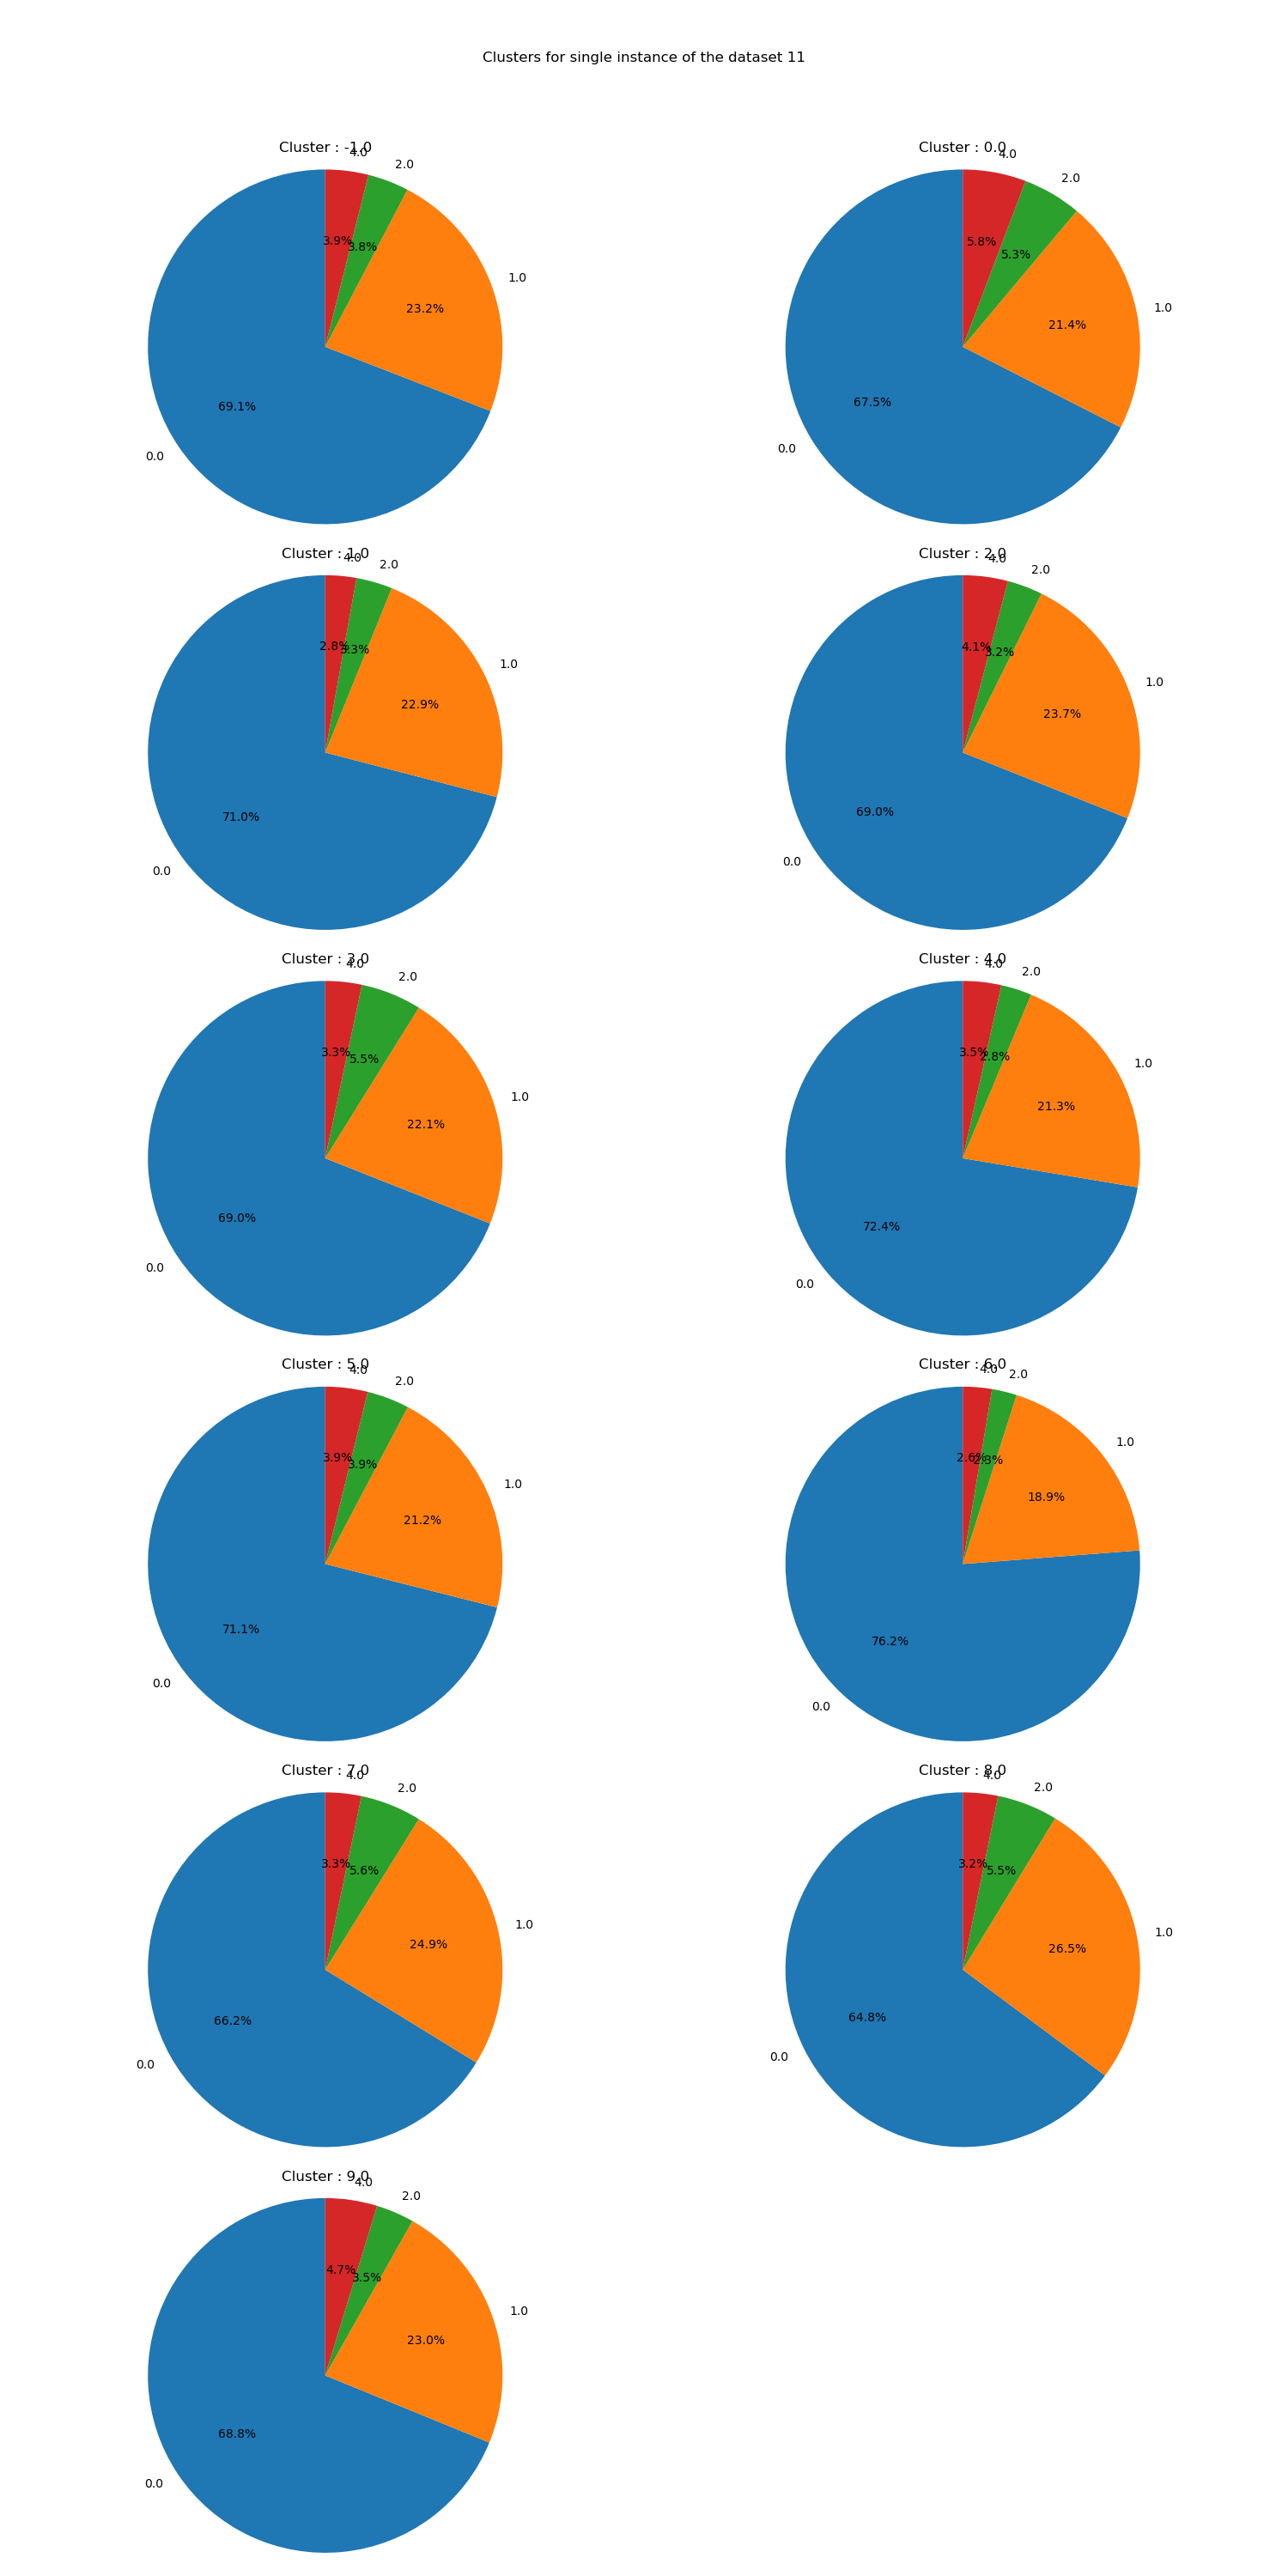
\includegraphics[width=0.8\linewidth]{img/annexes/11/clustering_pie_charts/single instance.png}} \\
\end{longtable}


\subsection{13 chunk\_semantic\_embedding (filtered chunk size)}

\begin{longtable}{|c|c|c|c|c|}
\caption{single instance Clustering Results on 13} \label{tab:13_single_instance_clustering_results}\\
\hline
\multicolumn{5}{|c|}{\textbf{General Information}} \\
\hline
\multicolumn{2}{|c|}{Min Samples} & \multicolumn{3}{c|}{234} \\
\multicolumn{2}{|c|}{Total Duration} & \multicolumn{3}{c|}{4582.308006 s} \\
\hline
\multicolumn{5}{|c|}{\textbf{Clustering Information}} \\
\hline
EPS & Number of Clusters & Silhouette Score & Noise Points & Duration \\
0.01 & 9 & -0.16028672456741333 & 3187 & 914.751199 s\\
0.02 & 9 & -0.16060906648635864 & 3189 & 798.03534 s\\
0.03 & 9 & -0.16189861297607422 & 3197 & 910.878093 s\\
0.04 & 9 & -0.1636056900024414 & 3228 & 917.586341 s\\
0.05 & 9 & -0.1794627606868744 & 3717 & 1030.724957 s\\
\hline
\multicolumn{5}{|c|}{\textbf{Best EPS Information}} \\
\hline
0.01 & 9 & -0.16028672456741333 & 3187 & 914.751199 s\\
\hline
\multicolumn{5}{|c|}{\textbf{Label Association}} \\
\hline
Cluster ID & \multicolumn{2}{c|}{Label} & \multicolumn{2}{c|}{Number of Samples} \\
\hline
\multirow{4}{*}{-1.0} & \multicolumn{2}{c|}{0.0} & \multicolumn{2}{c|}{3153} \\
& \multicolumn{2}{c|}{1.0} & \multicolumn{2}{c|}{28} \\
& \multicolumn{2}{c|}{2.0} & \multicolumn{2}{c|}{5} \\
& \multicolumn{2}{c|}{4.0} & \multicolumn{2}{c|}{1} \\
\hline
\multirow{3}{*}{0.0} & \multicolumn{2}{c|}{0.0} & \multicolumn{2}{c|}{514} \\
& \multicolumn{2}{c|}{1.0} & \multicolumn{2}{c|}{5} \\
& \multicolumn{2}{c|}{4.0} & \multicolumn{2}{c|}{1} \\
\hline
\multirow{2}{*}{1.0} & \multicolumn{2}{c|}{0.0} & \multicolumn{2}{c|}{248} \\
& \multicolumn{2}{c|}{1.0} & \multicolumn{2}{c|}{2} \\
\hline
\multirow{4}{*}{2.0} & \multicolumn{2}{c|}{0.0} & \multicolumn{2}{c|}{703} \\
& \multicolumn{2}{c|}{1.0} & \multicolumn{2}{c|}{4} \\
& \multicolumn{2}{c|}{2.0} & \multicolumn{2}{c|}{1} \\
& \multicolumn{2}{c|}{4.0} & \multicolumn{2}{c|}{2} \\
\hline
\multirow{3}{*}{3.0} & \multicolumn{2}{c|}{0.0} & \multicolumn{2}{c|}{558} \\
& \multicolumn{2}{c|}{1.0} & \multicolumn{2}{c|}{1} \\
& \multicolumn{2}{c|}{2.0} & \multicolumn{2}{c|}{1} \\
\hline
\multirow{3}{*}{4.0} & \multicolumn{2}{c|}{0.0} & \multicolumn{2}{c|}{538} \\
& \multicolumn{2}{c|}{1.0} & \multicolumn{2}{c|}{6} \\
& \multicolumn{2}{c|}{4.0} & \multicolumn{2}{c|}{4} \\
\hline
\multirow{3}{*}{5.0} & \multicolumn{2}{c|}{0.0} & \multicolumn{2}{c|}{247} \\
& \multicolumn{2}{c|}{1.0} & \multicolumn{2}{c|}{2} \\
& \multicolumn{2}{c|}{4.0} & \multicolumn{2}{c|}{1} \\
\hline
\multirow{3}{*}{6.0} & \multicolumn{2}{c|}{0.0} & \multicolumn{2}{c|}{401} \\
& \multicolumn{2}{c|}{1.0} & \multicolumn{2}{c|}{5} \\
& \multicolumn{2}{c|}{4.0} & \multicolumn{2}{c|}{1} \\
\hline
\multirow{3}{*}{7.0} & \multicolumn{2}{c|}{0.0} & \multicolumn{2}{c|}{460} \\
& \multicolumn{2}{c|}{1.0} & \multicolumn{2}{c|}{2} \\
& \multicolumn{2}{c|}{2.0} & \multicolumn{2}{c|}{1} \\
\hline
\multirow{3}{*}{8.0} & \multicolumn{2}{c|}{0.0} & \multicolumn{2}{c|}{596} \\
& \multicolumn{2}{c|}{1.0} & \multicolumn{2}{c|}{5} \\
& \multicolumn{2}{c|}{2.0} & \multicolumn{2}{c|}{2} \\
\hline
\multicolumn{5}{|c|}{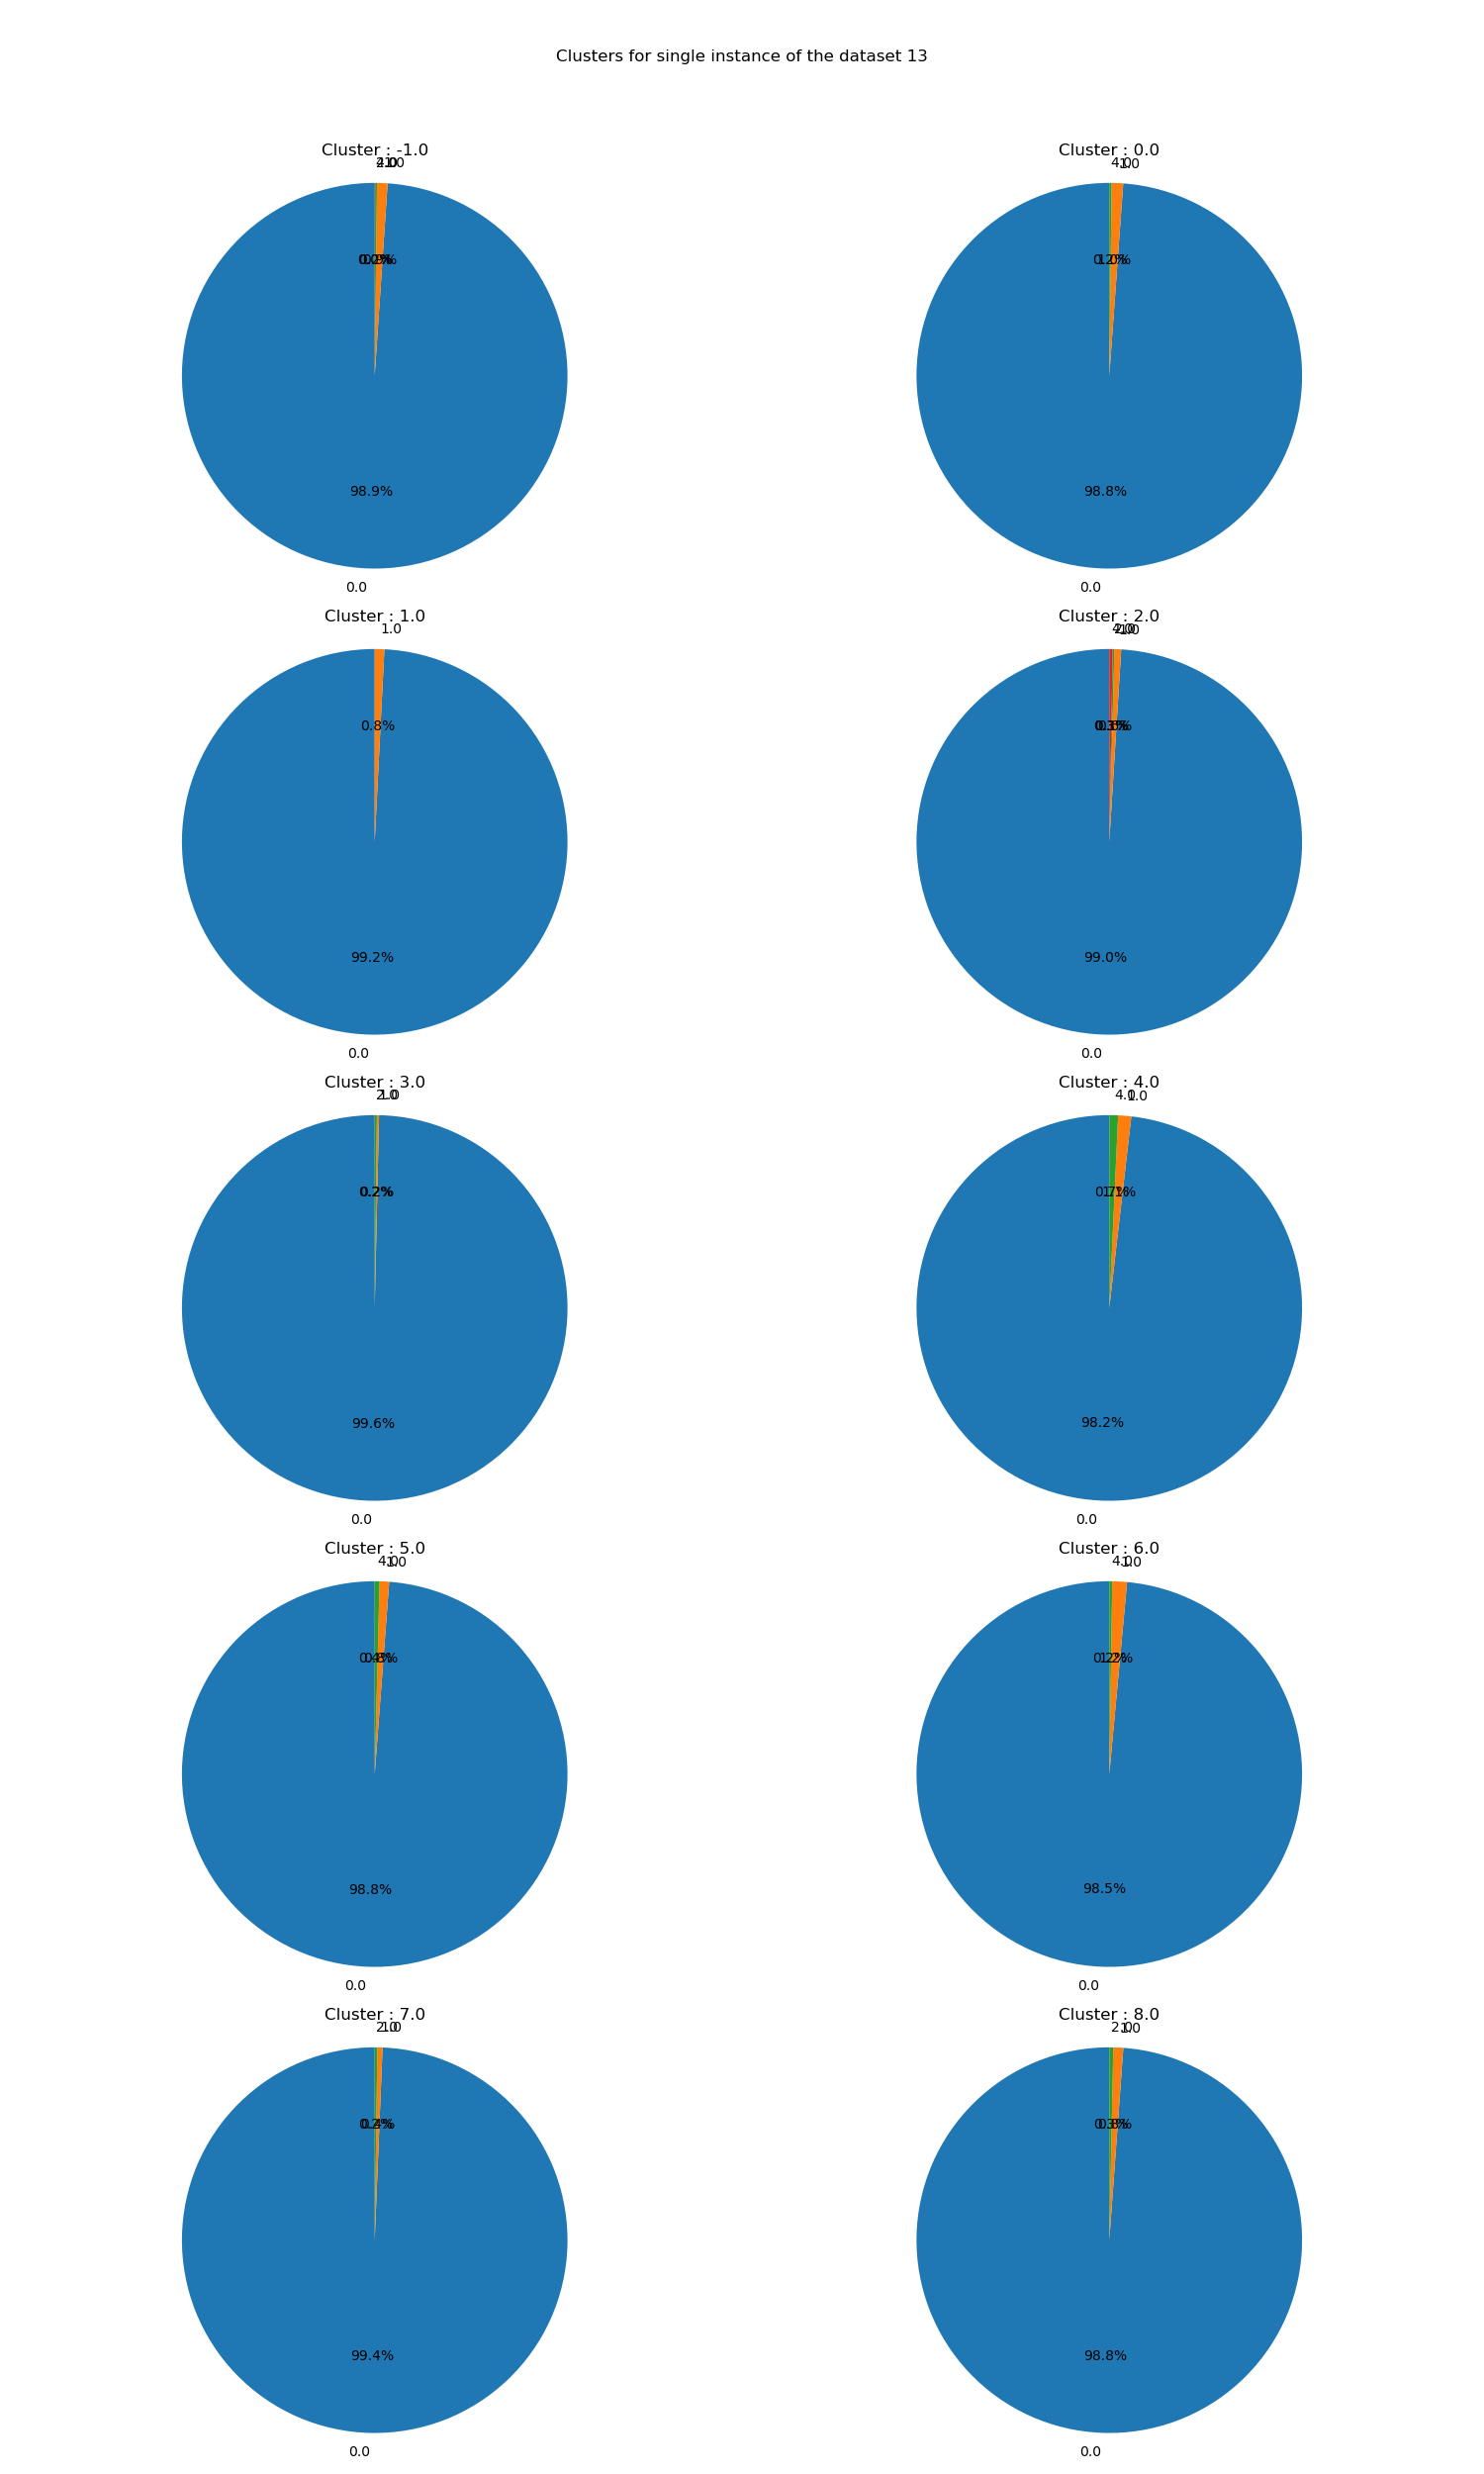
\includegraphics[width=0.8\linewidth]{img/annexes/13/clustering_pie_charts/single instance.png}} \\
\end{longtable}


\subsection{18 chunk\_statistic\_embedding (filtered entropy)}

\begin{longtable}{|c|c|c|c|c|}
\caption{single instance Clustering Results on 18} \label{tab:18_single_instance_clustering_results}\\
\hline
\multicolumn{5}{|c|}{\textbf{General Information}} \\
\hline
\multicolumn{2}{|c|}{Min Samples} & \multicolumn{3}{c|}{234} \\
\multicolumn{2}{|c|}{Total Duration} & \multicolumn{3}{c|}{4246.880698 s} \\
\hline
\multicolumn{5}{|c|}{\textbf{Clustering Information}} \\
\hline
EPS & Number of Clusters & Silhouette Score & Noise Points & Duration \\
0.01 & 7 & -0.14461402595043182 & 3665 & 792.918711 s\\
0.02 & 6 & -0.1517905294895172 & 3908 & 896.337555 s\\
0.03 & 6 & -0.15353043377399445 & 3915 & 855.336644 s\\
0.04 & 5 & -0.17628520727157593 & 4362 & 803.869787 s\\
0.05 & 4 & -0.2082502543926239 & 4967 & 894.490529 s\\
\hline
\multicolumn{5}{|c|}{\textbf{Best EPS Information}} \\
\hline
0.01 & 7 & -0.14461402595043182 & 3665 & 792.918711 s\\
\hline
\multicolumn{5}{|c|}{\textbf{Label Association}} \\
\hline
Cluster ID & \multicolumn{2}{c|}{Label} & \multicolumn{2}{c|}{Number of Samples} \\
\hline
\multirow{4}{*}{-1.0} & \multicolumn{2}{c|}{0.0} & \multicolumn{2}{c|}{2911} \\
& \multicolumn{2}{c|}{1.0} & \multicolumn{2}{c|}{578} \\
& \multicolumn{2}{c|}{2.0} & \multicolumn{2}{c|}{90} \\
& \multicolumn{2}{c|}{4.0} & \multicolumn{2}{c|}{86} \\
\hline
\multirow{4}{*}{0.0} & \multicolumn{2}{c|}{0.0} & \multicolumn{2}{c|}{192} \\
& \multicolumn{2}{c|}{1.0} & \multicolumn{2}{c|}{31} \\
& \multicolumn{2}{c|}{2.0} & \multicolumn{2}{c|}{5} \\
& \multicolumn{2}{c|}{4.0} & \multicolumn{2}{c|}{13} \\
\hline
\multirow{4}{*}{1.0} & \multicolumn{2}{c|}{0.0} & \multicolumn{2}{c|}{225} \\
& \multicolumn{2}{c|}{1.0} & \multicolumn{2}{c|}{49} \\
& \multicolumn{2}{c|}{2.0} & \multicolumn{2}{c|}{7} \\
& \multicolumn{2}{c|}{4.0} & \multicolumn{2}{c|}{7} \\
\hline
\multirow{4}{*}{2.0} & \multicolumn{2}{c|}{0.0} & \multicolumn{2}{c|}{472} \\
& \multicolumn{2}{c|}{1.0} & \multicolumn{2}{c|}{95} \\
& \multicolumn{2}{c|}{2.0} & \multicolumn{2}{c|}{23} \\
& \multicolumn{2}{c|}{4.0} & \multicolumn{2}{c|}{15} \\
\hline
\multirow{4}{*}{3.0} & \multicolumn{2}{c|}{0.0} & \multicolumn{2}{c|}{783} \\
& \multicolumn{2}{c|}{1.0} & \multicolumn{2}{c|}{168} \\
& \multicolumn{2}{c|}{2.0} & \multicolumn{2}{c|}{21} \\
& \multicolumn{2}{c|}{4.0} & \multicolumn{2}{c|}{30} \\
\hline
\multirow{4}{*}{4.0} & \multicolumn{2}{c|}{0.0} & \multicolumn{2}{c|}{362} \\
& \multicolumn{2}{c|}{1.0} & \multicolumn{2}{c|}{72} \\
& \multicolumn{2}{c|}{2.0} & \multicolumn{2}{c|}{6} \\
& \multicolumn{2}{c|}{4.0} & \multicolumn{2}{c|}{7} \\
\hline
\multirow{4}{*}{5.0} & \multicolumn{2}{c|}{0.0} & \multicolumn{2}{c|}{302} \\
& \multicolumn{2}{c|}{1.0} & \multicolumn{2}{c|}{54} \\
& \multicolumn{2}{c|}{2.0} & \multicolumn{2}{c|}{14} \\
& \multicolumn{2}{c|}{4.0} & \multicolumn{2}{c|}{11} \\
\hline
\multirow{4}{*}{6.0} & \multicolumn{2}{c|}{0.0} & \multicolumn{2}{c|}{679} \\
& \multicolumn{2}{c|}{1.0} & \multicolumn{2}{c|}{132} \\
& \multicolumn{2}{c|}{2.0} & \multicolumn{2}{c|}{31} \\
& \multicolumn{2}{c|}{4.0} & \multicolumn{2}{c|}{27} \\
\hline
\multicolumn{5}{|c|}{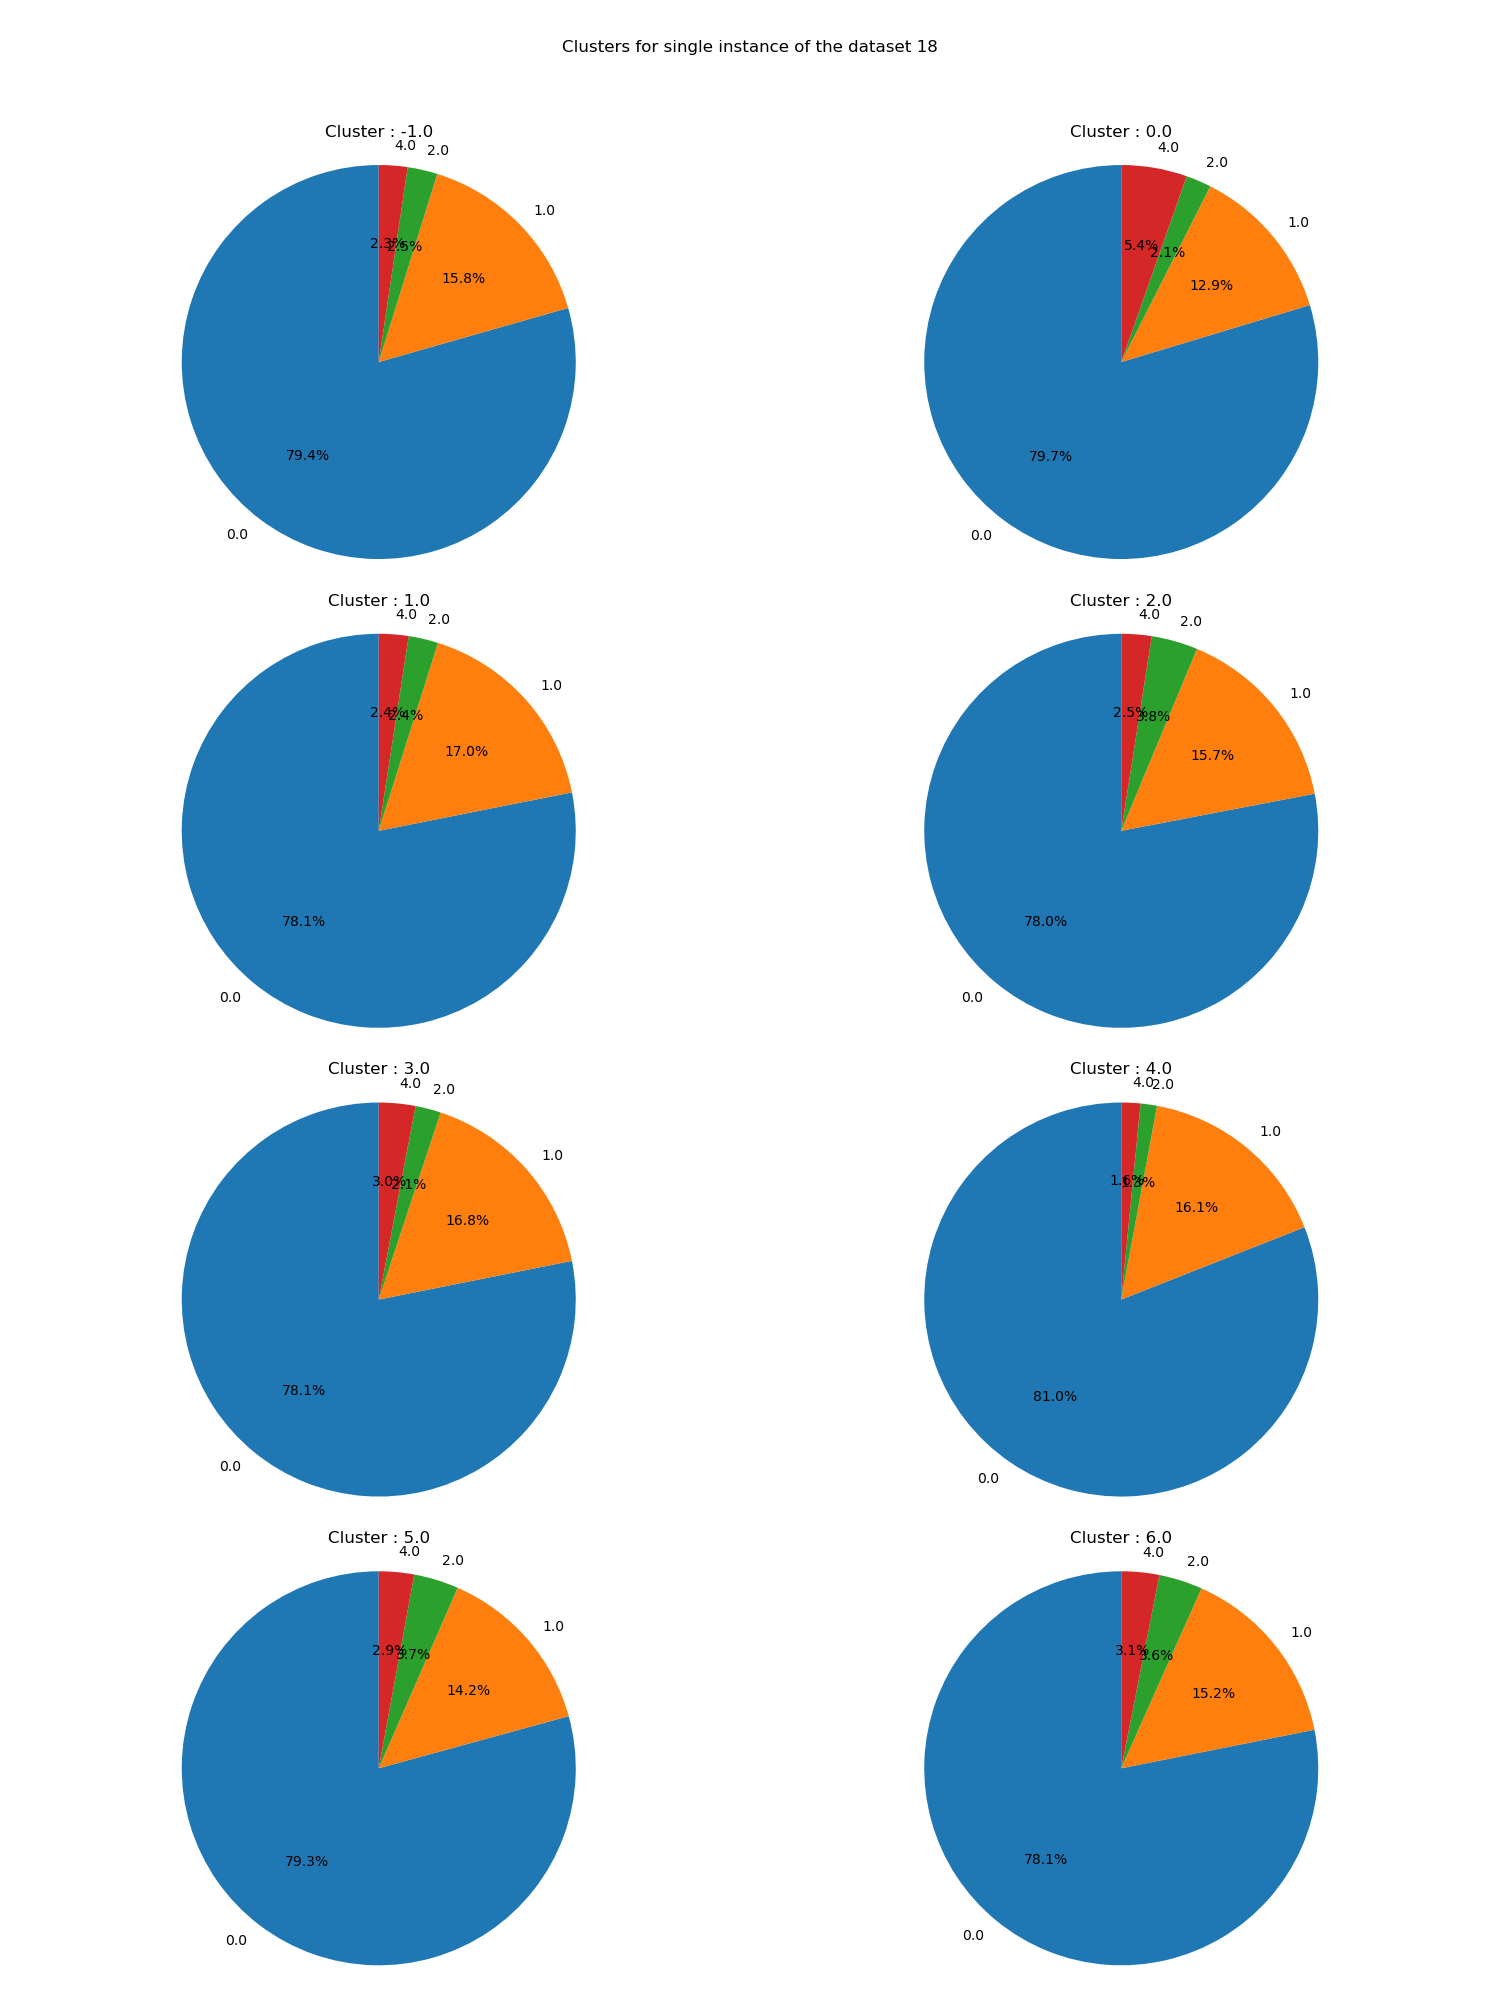
\includegraphics[width=0.8\linewidth]{img/annexes/18/clustering_pie_charts/single instance.png}} \\
\end{longtable}


\subsection{19 chunk\_statistic\_embedding (filtered entropy and chunk size)}

\begin{longtable}{|c|c|c|c|c|}
\caption{single instance Clustering Results on 19} \label{tab:19_single_instance_clustering_results}\\
\hline
\multicolumn{5}{|c|}{\textbf{General Information}} \\
\hline
\multicolumn{2}{|c|}{Min Samples} & \multicolumn{3}{c|}{234} \\
\multicolumn{2}{|c|}{Total Duration} & \multicolumn{3}{c|}{3692.032057 s} \\
\hline
\multicolumn{5}{|c|}{\textbf{Clustering Information}} \\
\hline
EPS & Number of Clusters & Silhouette Score & Noise Points & Duration \\
0.01 & 5 & -0.05387001484632492 & 4377 & 725.941822 s\\
0.02 & 4 & -0.5301076173782349 & 5886 & 802.3415 s\\
0.03 & 4 & 0.33267366886138916 & 349 & 659.691798 s\\
0.04 & 3 & 0.16098101437091827 & 5245 & 765.921124 s\\
0.05 & 3 & 0.11182425171136856 & 5531 & 733.477938 s\\
\hline
\multicolumn{5}{|c|}{\textbf{Best EPS Information}} \\
\hline
0.03 & 4 & 0.33267366886138916 & 349 & 659.691798 s\\
\hline
\multicolumn{5}{|c|}{\textbf{Label Association}} \\
\hline
Cluster ID & \multicolumn{2}{c|}{Label} & \multicolumn{2}{c|}{Number of Samples} \\
\hline
\multirow{4}{*}{-1.0} & \multicolumn{2}{c|}{0.0} & \multicolumn{2}{c|}{232} \\
& \multicolumn{2}{c|}{1.0} & \multicolumn{2}{c|}{83} \\
& \multicolumn{2}{c|}{2.0} & \multicolumn{2}{c|}{17} \\
& \multicolumn{2}{c|}{4.0} & \multicolumn{2}{c|}{17} \\
\hline
\multirow{4}{*}{0.0} & \multicolumn{2}{c|}{0.0} & \multicolumn{2}{c|}{3398} \\
& \multicolumn{2}{c|}{1.0} & \multicolumn{2}{c|}{1130} \\
& \multicolumn{2}{c|}{2.0} & \multicolumn{2}{c|}{178} \\
& \multicolumn{2}{c|}{4.0} & \multicolumn{2}{c|}{190} \\
\hline
\multirow{4}{*}{1.0} & \multicolumn{2}{c|}{0.0} & \multicolumn{2}{c|}{882} \\
& \multicolumn{2}{c|}{1.0} & \multicolumn{2}{c|}{267} \\
& \multicolumn{2}{c|}{2.0} & \multicolumn{2}{c|}{46} \\
& \multicolumn{2}{c|}{4.0} & \multicolumn{2}{c|}{47} \\
\hline
\multirow{4}{*}{2.0} & \multicolumn{2}{c|}{0.0} & \multicolumn{2}{c|}{260} \\
& \multicolumn{2}{c|}{1.0} & \multicolumn{2}{c|}{83} \\
& \multicolumn{2}{c|}{2.0} & \multicolumn{2}{c|}{12} \\
& \multicolumn{2}{c|}{4.0} & \multicolumn{2}{c|}{11} \\
\hline
\multirow{4}{*}{3.0} & \multicolumn{2}{c|}{0.0} & \multicolumn{2}{c|}{445} \\
& \multicolumn{2}{c|}{1.0} & \multicolumn{2}{c|}{148} \\
& \multicolumn{2}{c|}{2.0} & \multicolumn{2}{c|}{32} \\
& \multicolumn{2}{c|}{4.0} & \multicolumn{2}{c|}{20} \\
\hline
\multicolumn{5}{|c|}{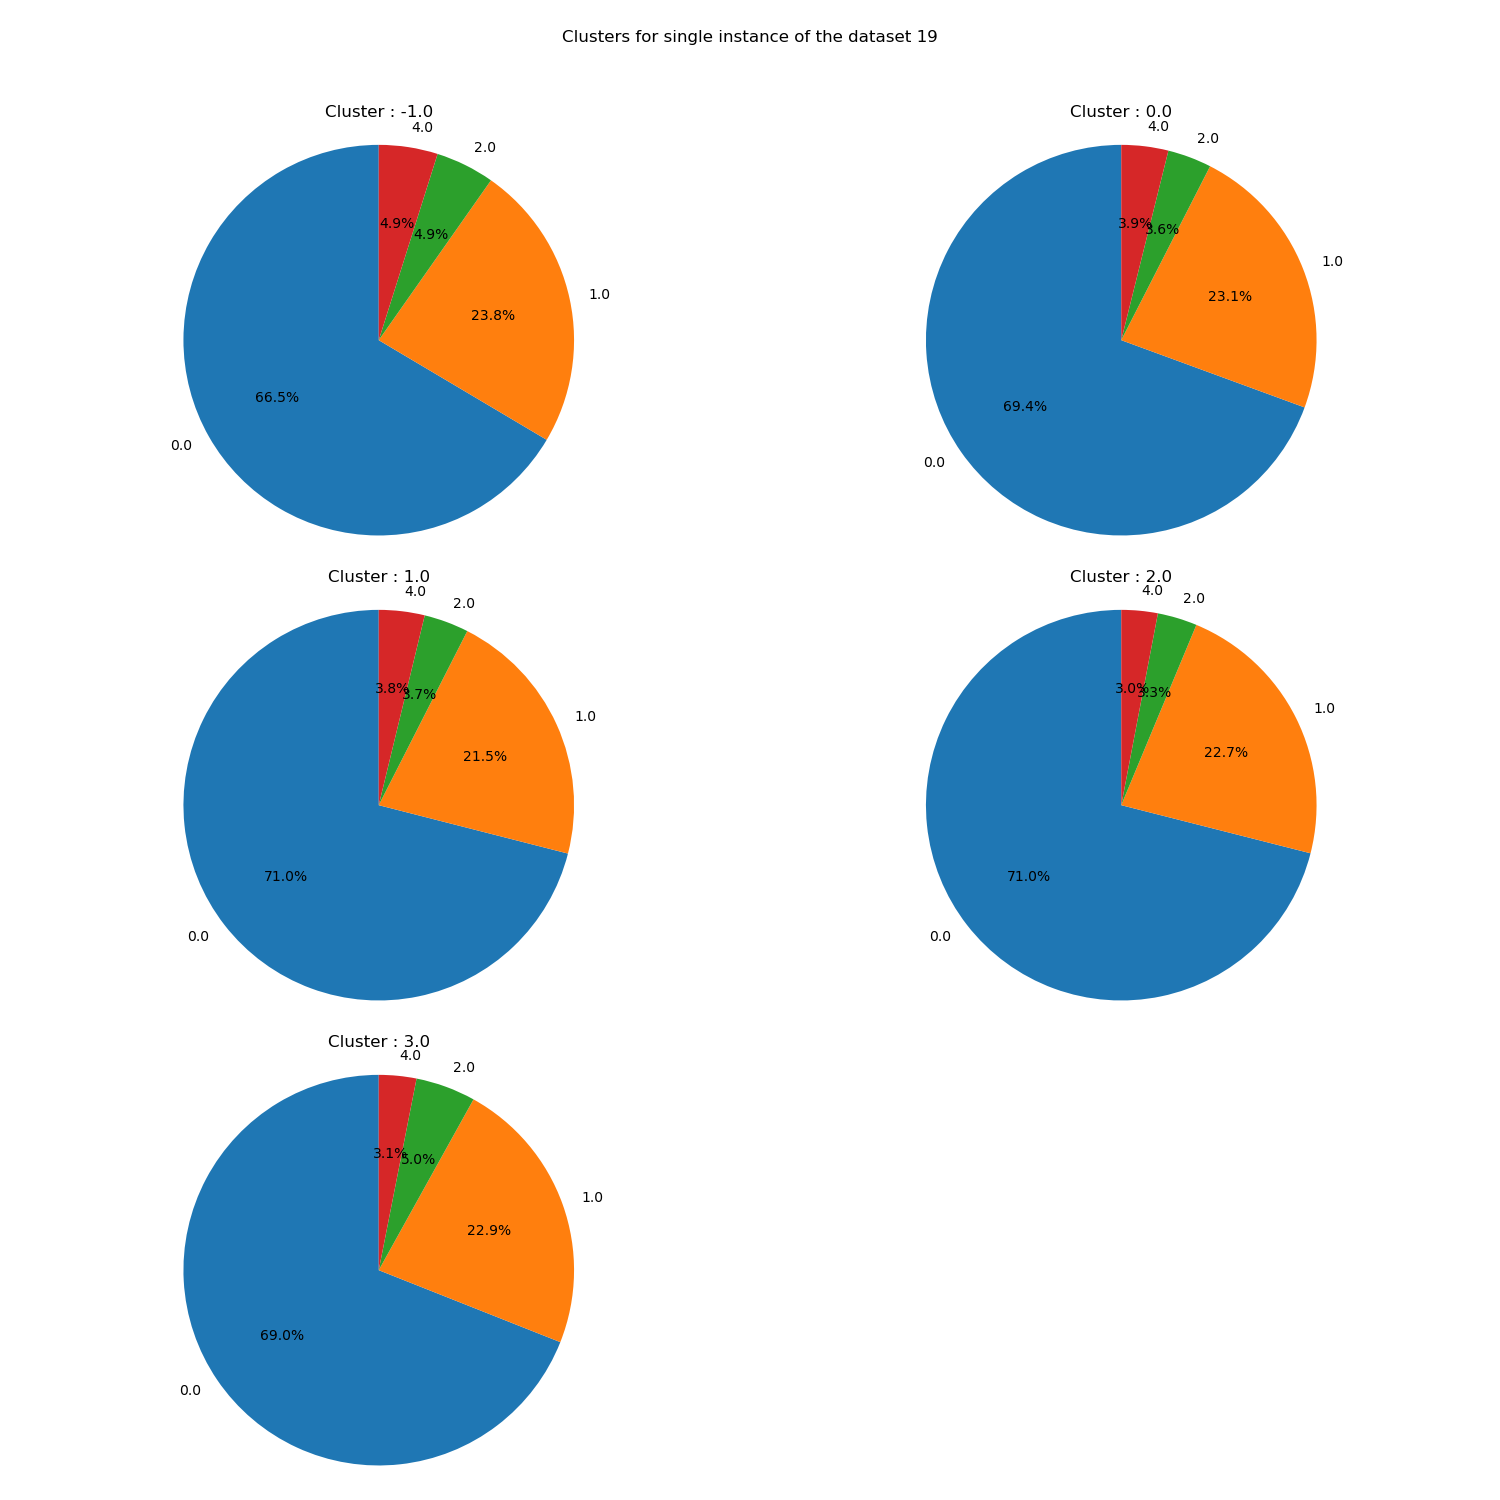
\includegraphics[width=0.8\linewidth]{img/annexes/19/clustering_pie_charts/single instance.png}} \\
\end{longtable}


\subsection{21 chunk\_start\_bytes\_embedding (filtered chunk size)}

\begin{longtable}{|c|c|c|c|c|}
\caption{single instance Clustering Results on 21} \label{tab:21_single_instance_clustering_results}\\
\hline
\multicolumn{5}{|c|}{\textbf{General Information}} \\
\hline
\multicolumn{2}{|c|}{Min Samples} & \multicolumn{3}{c|}{234} \\
\multicolumn{2}{|c|}{Total Duration} & \multicolumn{3}{c|}{3782.232716 s} \\
\hline
\multicolumn{5}{|c|}{\textbf{Clustering Information}} \\
\hline
EPS & Number of Clusters & Silhouette Score & Noise Points & Duration \\
0.01 & 5 & -0.183935284614563 & 4779 & 719.704639 s\\
0.02 & 2 & -0.17470110952854156 & 6289 & 779.895787 s\\
0.03 & 2 & -0.12927506864070892 & 5912 & 757.454194 s\\
0.04 & 2 & -0.13758240640163422 & 5945 & 771.111239 s\\
0.05 & 2 & 0.6121783256530762 & 496 & 742.290916 s\\
\hline
\multicolumn{5}{|c|}{\textbf{Best EPS Information}} \\
\hline
0.05 & 2 & 0.6121783256530762 & 496 & 742.290916 s\\
\hline
\multicolumn{5}{|c|}{\textbf{Label Association}} \\
\hline
Cluster ID & \multicolumn{2}{c|}{Label} & \multicolumn{2}{c|}{Number of Samples} \\
\hline
\multirow{3}{*}{-1.0} & \multicolumn{2}{c|}{0.0} & \multicolumn{2}{c|}{493} \\
& \multicolumn{2}{c|}{1.0} & \multicolumn{2}{c|}{2} \\
& \multicolumn{2}{c|}{4.0} & \multicolumn{2}{c|}{1} \\
\hline
\multirow{4}{*}{0.0} & \multicolumn{2}{c|}{0.0} & \multicolumn{2}{c|}{6397} \\
& \multicolumn{2}{c|}{1.0} & \multicolumn{2}{c|}{27} \\
& \multicolumn{2}{c|}{2.0} & \multicolumn{2}{c|}{5} \\
& \multicolumn{2}{c|}{4.0} & \multicolumn{2}{c|}{3} \\
\hline
\multirow{3}{*}{1.0} & \multicolumn{2}{c|}{0.0} & \multicolumn{2}{c|}{568} \\
& \multicolumn{2}{c|}{1.0} & \multicolumn{2}{c|}{1} \\
& \multicolumn{2}{c|}{4.0} & \multicolumn{2}{c|}{1} \\
\hline
\multicolumn{5}{|c|}{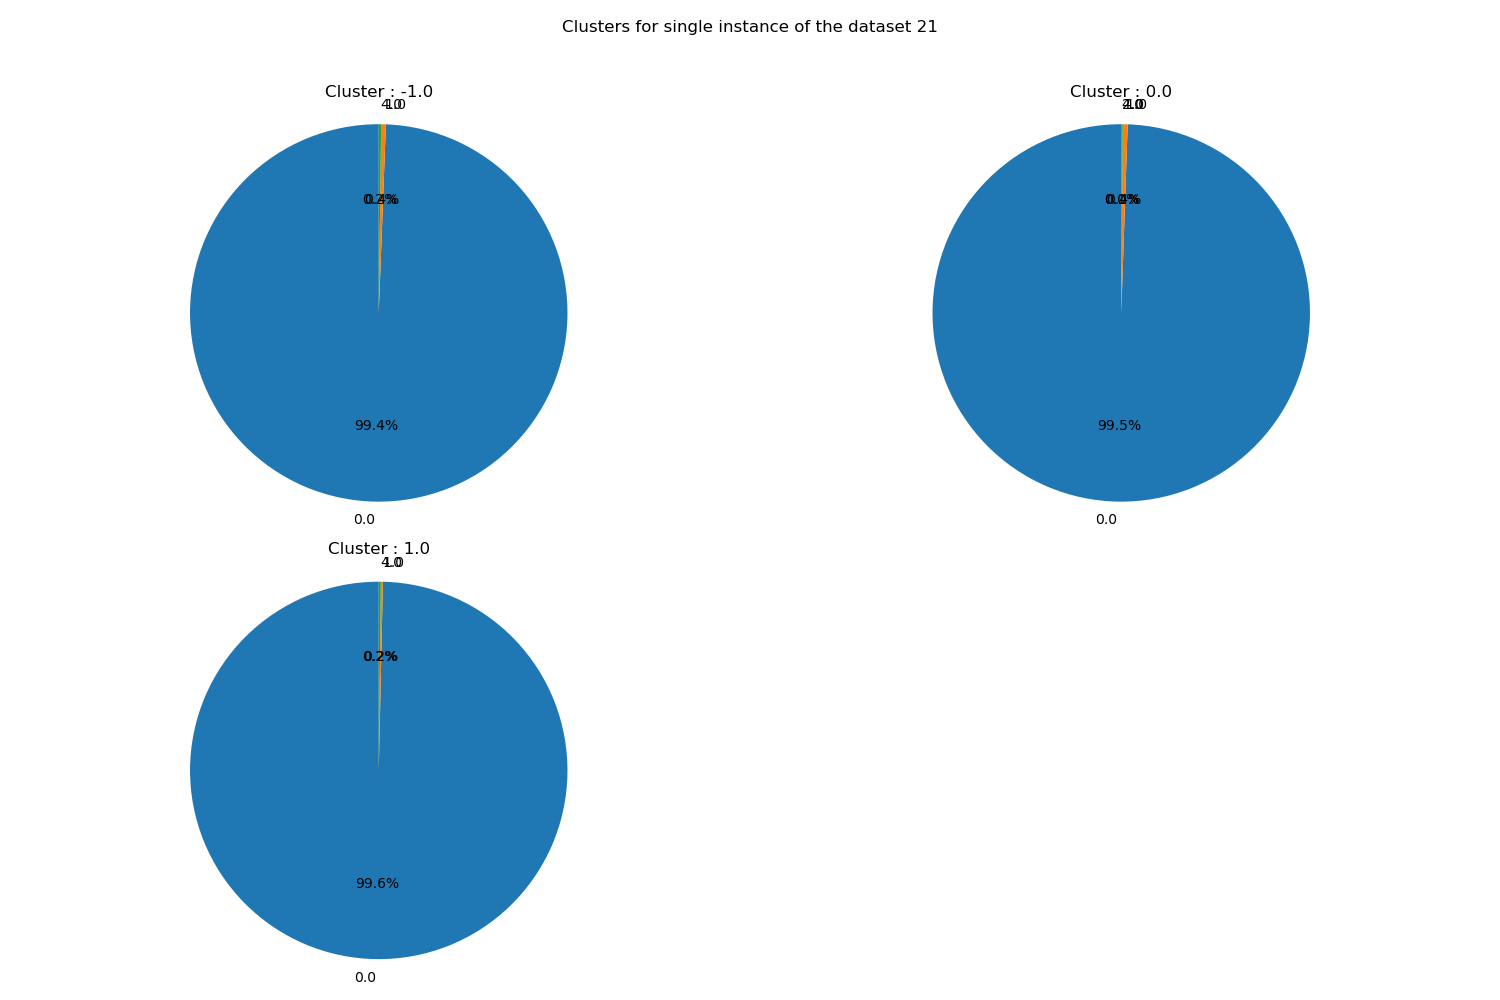
\includegraphics[width=0.8\linewidth]{img/annexes/21/clustering_pie_charts/single instance.png}} \\
\end{longtable}


\subsection{22 chunk\_start\_bytes\_embedding (filtered entropy)}

\begin{longtable}{|c|c|c|c|c|}
\caption{single instance Clustering Results on 22} \label{tab:22_single_instance_clustering_results}\\
\hline
\multicolumn{5}{|c|}{\textbf{General Information}} \\
\hline
\multicolumn{2}{|c|}{Min Samples} & \multicolumn{3}{c|}{234} \\
\multicolumn{2}{|c|}{Total Duration} & \multicolumn{3}{c|}{4211.284218 s} \\
\hline
\multicolumn{5}{|c|}{\textbf{Clustering Information}} \\
\hline
EPS & Number of Clusters & Silhouette Score & Noise Points & Duration \\
0.01 & 9 & -0.1507883220911026 & 3317 & 747.264132 s\\
0.02 & 7 & 0.08796403557062149 & 3552 & 905.581793 s\\
0.03 & 6 & 0.0919799953699112 & 3946 & 892.185804 s\\
0.04 & 6 & -0.014515701681375504 & 4335 & 812.500732 s\\
0.05 & 5 & -0.04107537493109703 & 4705 & 849.840643 s\\
\hline
\multicolumn{5}{|c|}{\textbf{Best EPS Information}} \\
\hline
0.03 & 6 & 0.0919799953699112 & 3946 & 892.185804 s\\
\hline
\multicolumn{5}{|c|}{\textbf{Label Association}} \\
\hline
Cluster ID & \multicolumn{2}{c|}{Label} & \multicolumn{2}{c|}{Number of Samples} \\
\hline
\multirow{4}{*}{-1.0} & \multicolumn{2}{c|}{0.0} & \multicolumn{2}{c|}{3109} \\
& \multicolumn{2}{c|}{1.0} & \multicolumn{2}{c|}{628} \\
& \multicolumn{2}{c|}{2.0} & \multicolumn{2}{c|}{109} \\
& \multicolumn{2}{c|}{4.0} & \multicolumn{2}{c|}{100} \\
\hline
\multirow{4}{*}{0.0} & \multicolumn{2}{c|}{0.0} & \multicolumn{2}{c|}{262} \\
& \multicolumn{2}{c|}{1.0} & \multicolumn{2}{c|}{68} \\
& \multicolumn{2}{c|}{2.0} & \multicolumn{2}{c|}{11} \\
& \multicolumn{2}{c|}{4.0} & \multicolumn{2}{c|}{10} \\
\hline
\multirow{4}{*}{1.0} & \multicolumn{2}{c|}{0.0} & \multicolumn{2}{c|}{491} \\
& \multicolumn{2}{c|}{1.0} & \multicolumn{2}{c|}{79} \\
& \multicolumn{2}{c|}{2.0} & \multicolumn{2}{c|}{21} \\
& \multicolumn{2}{c|}{4.0} & \multicolumn{2}{c|}{19} \\
\hline
\multirow{4}{*}{2.0} & \multicolumn{2}{c|}{0.0} & \multicolumn{2}{c|}{922} \\
& \multicolumn{2}{c|}{1.0} & \multicolumn{2}{c|}{178} \\
& \multicolumn{2}{c|}{2.0} & \multicolumn{2}{c|}{13} \\
& \multicolumn{2}{c|}{4.0} & \multicolumn{2}{c|}{33} \\
\hline
\multirow{4}{*}{3.0} & \multicolumn{2}{c|}{0.0} & \multicolumn{2}{c|}{218} \\
& \multicolumn{2}{c|}{1.0} & \multicolumn{2}{c|}{50} \\
& \multicolumn{2}{c|}{2.0} & \multicolumn{2}{c|}{9} \\
& \multicolumn{2}{c|}{4.0} & \multicolumn{2}{c|}{7} \\
\hline
\multirow{4}{*}{4.0} & \multicolumn{2}{c|}{0.0} & \multicolumn{2}{c|}{396} \\
& \multicolumn{2}{c|}{1.0} & \multicolumn{2}{c|}{76} \\
& \multicolumn{2}{c|}{2.0} & \multicolumn{2}{c|}{13} \\
& \multicolumn{2}{c|}{4.0} & \multicolumn{2}{c|}{13} \\
\hline
\multirow{4}{*}{5.0} & \multicolumn{2}{c|}{0.0} & \multicolumn{2}{c|}{524} \\
& \multicolumn{2}{c|}{1.0} & \multicolumn{2}{c|}{103} \\
& \multicolumn{2}{c|}{2.0} & \multicolumn{2}{c|}{21} \\
& \multicolumn{2}{c|}{4.0} & \multicolumn{2}{c|}{15} \\
\hline
\multicolumn{5}{|c|}{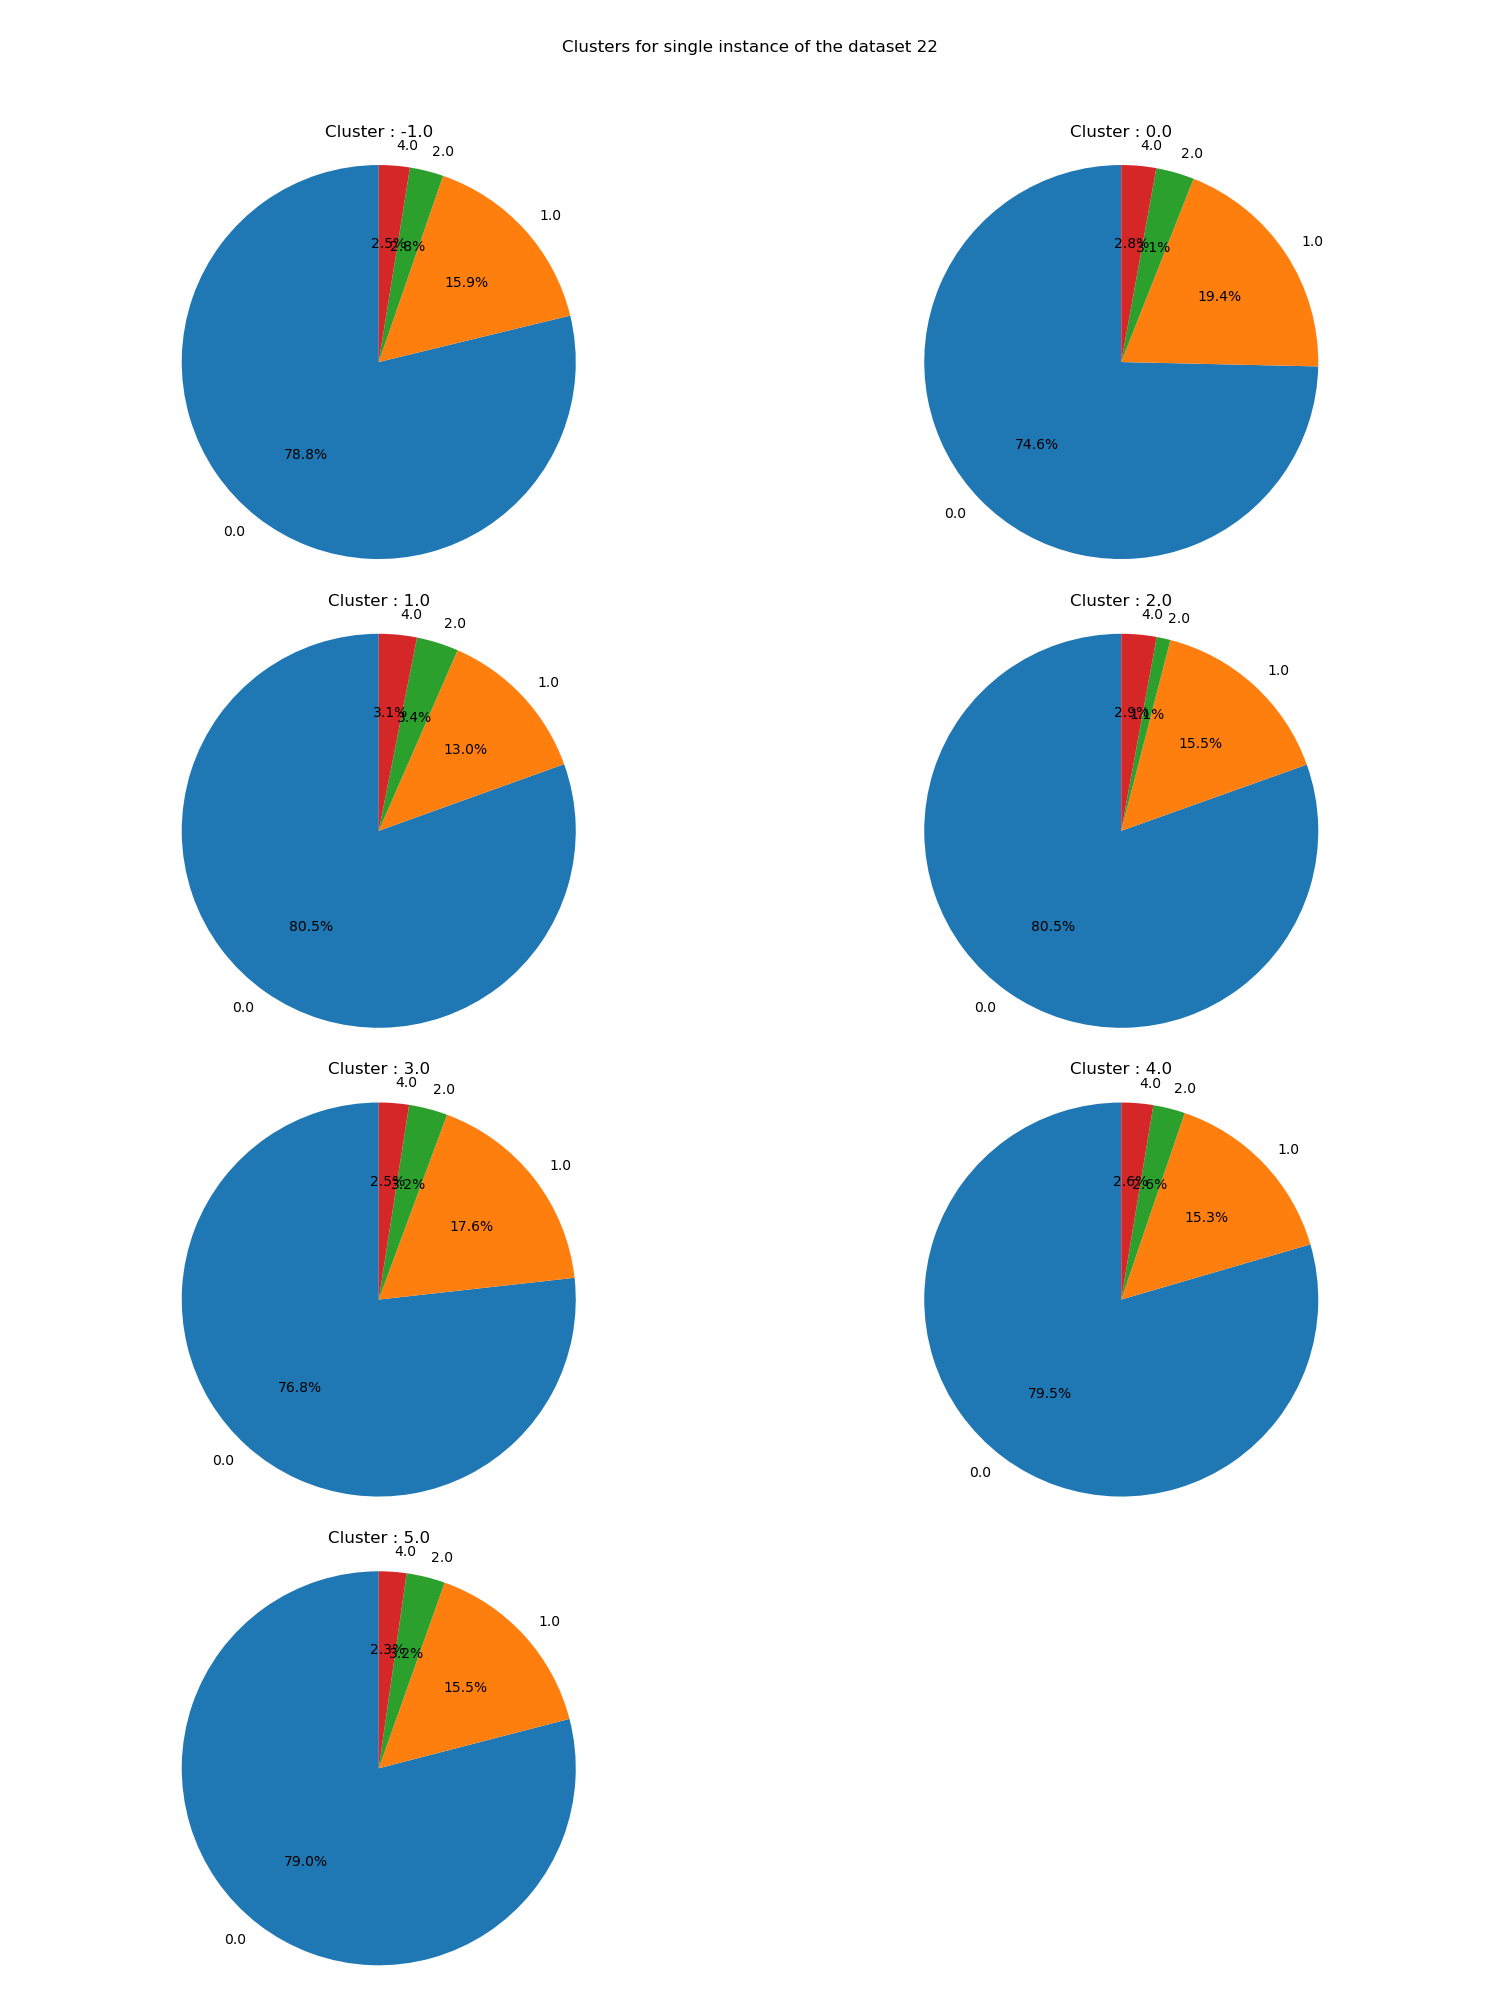
\includegraphics[width=0.8\linewidth]{img/annexes/22/clustering_pie_charts/single instance.png}} \\
\end{longtable}


\subsection{23 chunk\_start\_bytes\_embedding (filtered entropy and chunk size)}

\begin{longtable}{|c|c|c|c|c|}
\caption{single instance Clustering Results on 23} \label{tab:23_single_instance_clustering_results}\\
\hline
\multicolumn{5}{|c|}{\textbf{General Information}} \\
\hline
\multicolumn{2}{|c|}{Min Samples} & \multicolumn{3}{c|}{234} \\
\multicolumn{2}{|c|}{Total Duration} & \multicolumn{3}{c|}{4332.212255 s} \\
\hline
\multicolumn{5}{|c|}{\textbf{Clustering Information}} \\
\hline
EPS & Number of Clusters & Silhouette Score & Noise Points & Duration \\
0.01 & 9 & -0.08887682855129242 & 3521 & 856.295821 s\\
0.02 & 8 & -0.10835617035627365 & 4194 & 1001.794516 s\\
0.03 & 8 & -0.12353134900331497 & 4378 & 891.398419 s\\
0.04 & 8 & -0.12524381279945374 & 4395 & 799.487674 s\\
0.05 & 8 & -0.12136006355285645 & 4405 & 777.880095 s\\
\hline
\multicolumn{5}{|c|}{\textbf{Best EPS Information}} \\
\hline
0.01 & 9 & -0.08887682855129242 & 3521 & 856.295821 s\\
\hline
\multicolumn{5}{|c|}{\textbf{Label Association}} \\
\hline
Cluster ID & \multicolumn{2}{c|}{Label} & \multicolumn{2}{c|}{Number of Samples} \\
\hline
\multirow{4}{*}{-1.0} & \multicolumn{2}{c|}{0.0} & \multicolumn{2}{c|}{2448} \\
& \multicolumn{2}{c|}{1.0} & \multicolumn{2}{c|}{817} \\
& \multicolumn{2}{c|}{2.0} & \multicolumn{2}{c|}{136} \\
& \multicolumn{2}{c|}{4.0} & \multicolumn{2}{c|}{120} \\
\hline
\multirow{4}{*}{0.0} & \multicolumn{2}{c|}{0.0} & \multicolumn{2}{c|}{270} \\
& \multicolumn{2}{c|}{1.0} & \multicolumn{2}{c|}{86} \\
& \multicolumn{2}{c|}{2.0} & \multicolumn{2}{c|}{19} \\
& \multicolumn{2}{c|}{4.0} & \multicolumn{2}{c|}{11} \\
\hline
\multirow{4}{*}{1.0} & \multicolumn{2}{c|}{0.0} & \multicolumn{2}{c|}{264} \\
& \multicolumn{2}{c|}{1.0} & \multicolumn{2}{c|}{91} \\
& \multicolumn{2}{c|}{2.0} & \multicolumn{2}{c|}{14} \\
& \multicolumn{2}{c|}{4.0} & \multicolumn{2}{c|}{22} \\
\hline
\multirow{4}{*}{2.0} & \multicolumn{2}{c|}{0.0} & \multicolumn{2}{c|}{248} \\
& \multicolumn{2}{c|}{1.0} & \multicolumn{2}{c|}{86} \\
& \multicolumn{2}{c|}{2.0} & \multicolumn{2}{c|}{15} \\
& \multicolumn{2}{c|}{4.0} & \multicolumn{2}{c|}{14} \\
\hline
\multirow{4}{*}{3.0} & \multicolumn{2}{c|}{0.0} & \multicolumn{2}{c|}{249} \\
& \multicolumn{2}{c|}{1.0} & \multicolumn{2}{c|}{69} \\
& \multicolumn{2}{c|}{2.0} & \multicolumn{2}{c|}{9} \\
& \multicolumn{2}{c|}{4.0} & \multicolumn{2}{c|}{13} \\
\hline
\multirow{4}{*}{4.0} & \multicolumn{2}{c|}{0.0} & \multicolumn{2}{c|}{503} \\
& \multicolumn{2}{c|}{1.0} & \multicolumn{2}{c|}{158} \\
& \multicolumn{2}{c|}{2.0} & \multicolumn{2}{c|}{34} \\
& \multicolumn{2}{c|}{4.0} & \multicolumn{2}{c|}{34} \\
\hline
\multirow{4}{*}{5.0} & \multicolumn{2}{c|}{0.0} & \multicolumn{2}{c|}{247} \\
& \multicolumn{2}{c|}{1.0} & \multicolumn{2}{c|}{90} \\
& \multicolumn{2}{c|}{2.0} & \multicolumn{2}{c|}{12} \\
& \multicolumn{2}{c|}{4.0} & \multicolumn{2}{c|}{13} \\
\hline
\multirow{4}{*}{6.0} & \multicolumn{2}{c|}{0.0} & \multicolumn{2}{c|}{244} \\
& \multicolumn{2}{c|}{1.0} & \multicolumn{2}{c|}{101} \\
& \multicolumn{2}{c|}{2.0} & \multicolumn{2}{c|}{8} \\
& \multicolumn{2}{c|}{4.0} & \multicolumn{2}{c|}{15} \\
\hline
\multirow{4}{*}{7.0} & \multicolumn{2}{c|}{0.0} & \multicolumn{2}{c|}{375} \\
& \multicolumn{2}{c|}{1.0} & \multicolumn{2}{c|}{135} \\
& \multicolumn{2}{c|}{2.0} & \multicolumn{2}{c|}{17} \\
& \multicolumn{2}{c|}{4.0} & \multicolumn{2}{c|}{26} \\
\hline
\multirow{4}{*}{8.0} & \multicolumn{2}{c|}{0.0} & \multicolumn{2}{c|}{343} \\
& \multicolumn{2}{c|}{1.0} & \multicolumn{2}{c|}{98} \\
& \multicolumn{2}{c|}{2.0} & \multicolumn{2}{c|}{24} \\
& \multicolumn{2}{c|}{4.0} & \multicolumn{2}{c|}{20} \\
\hline
\multicolumn{5}{|c|}{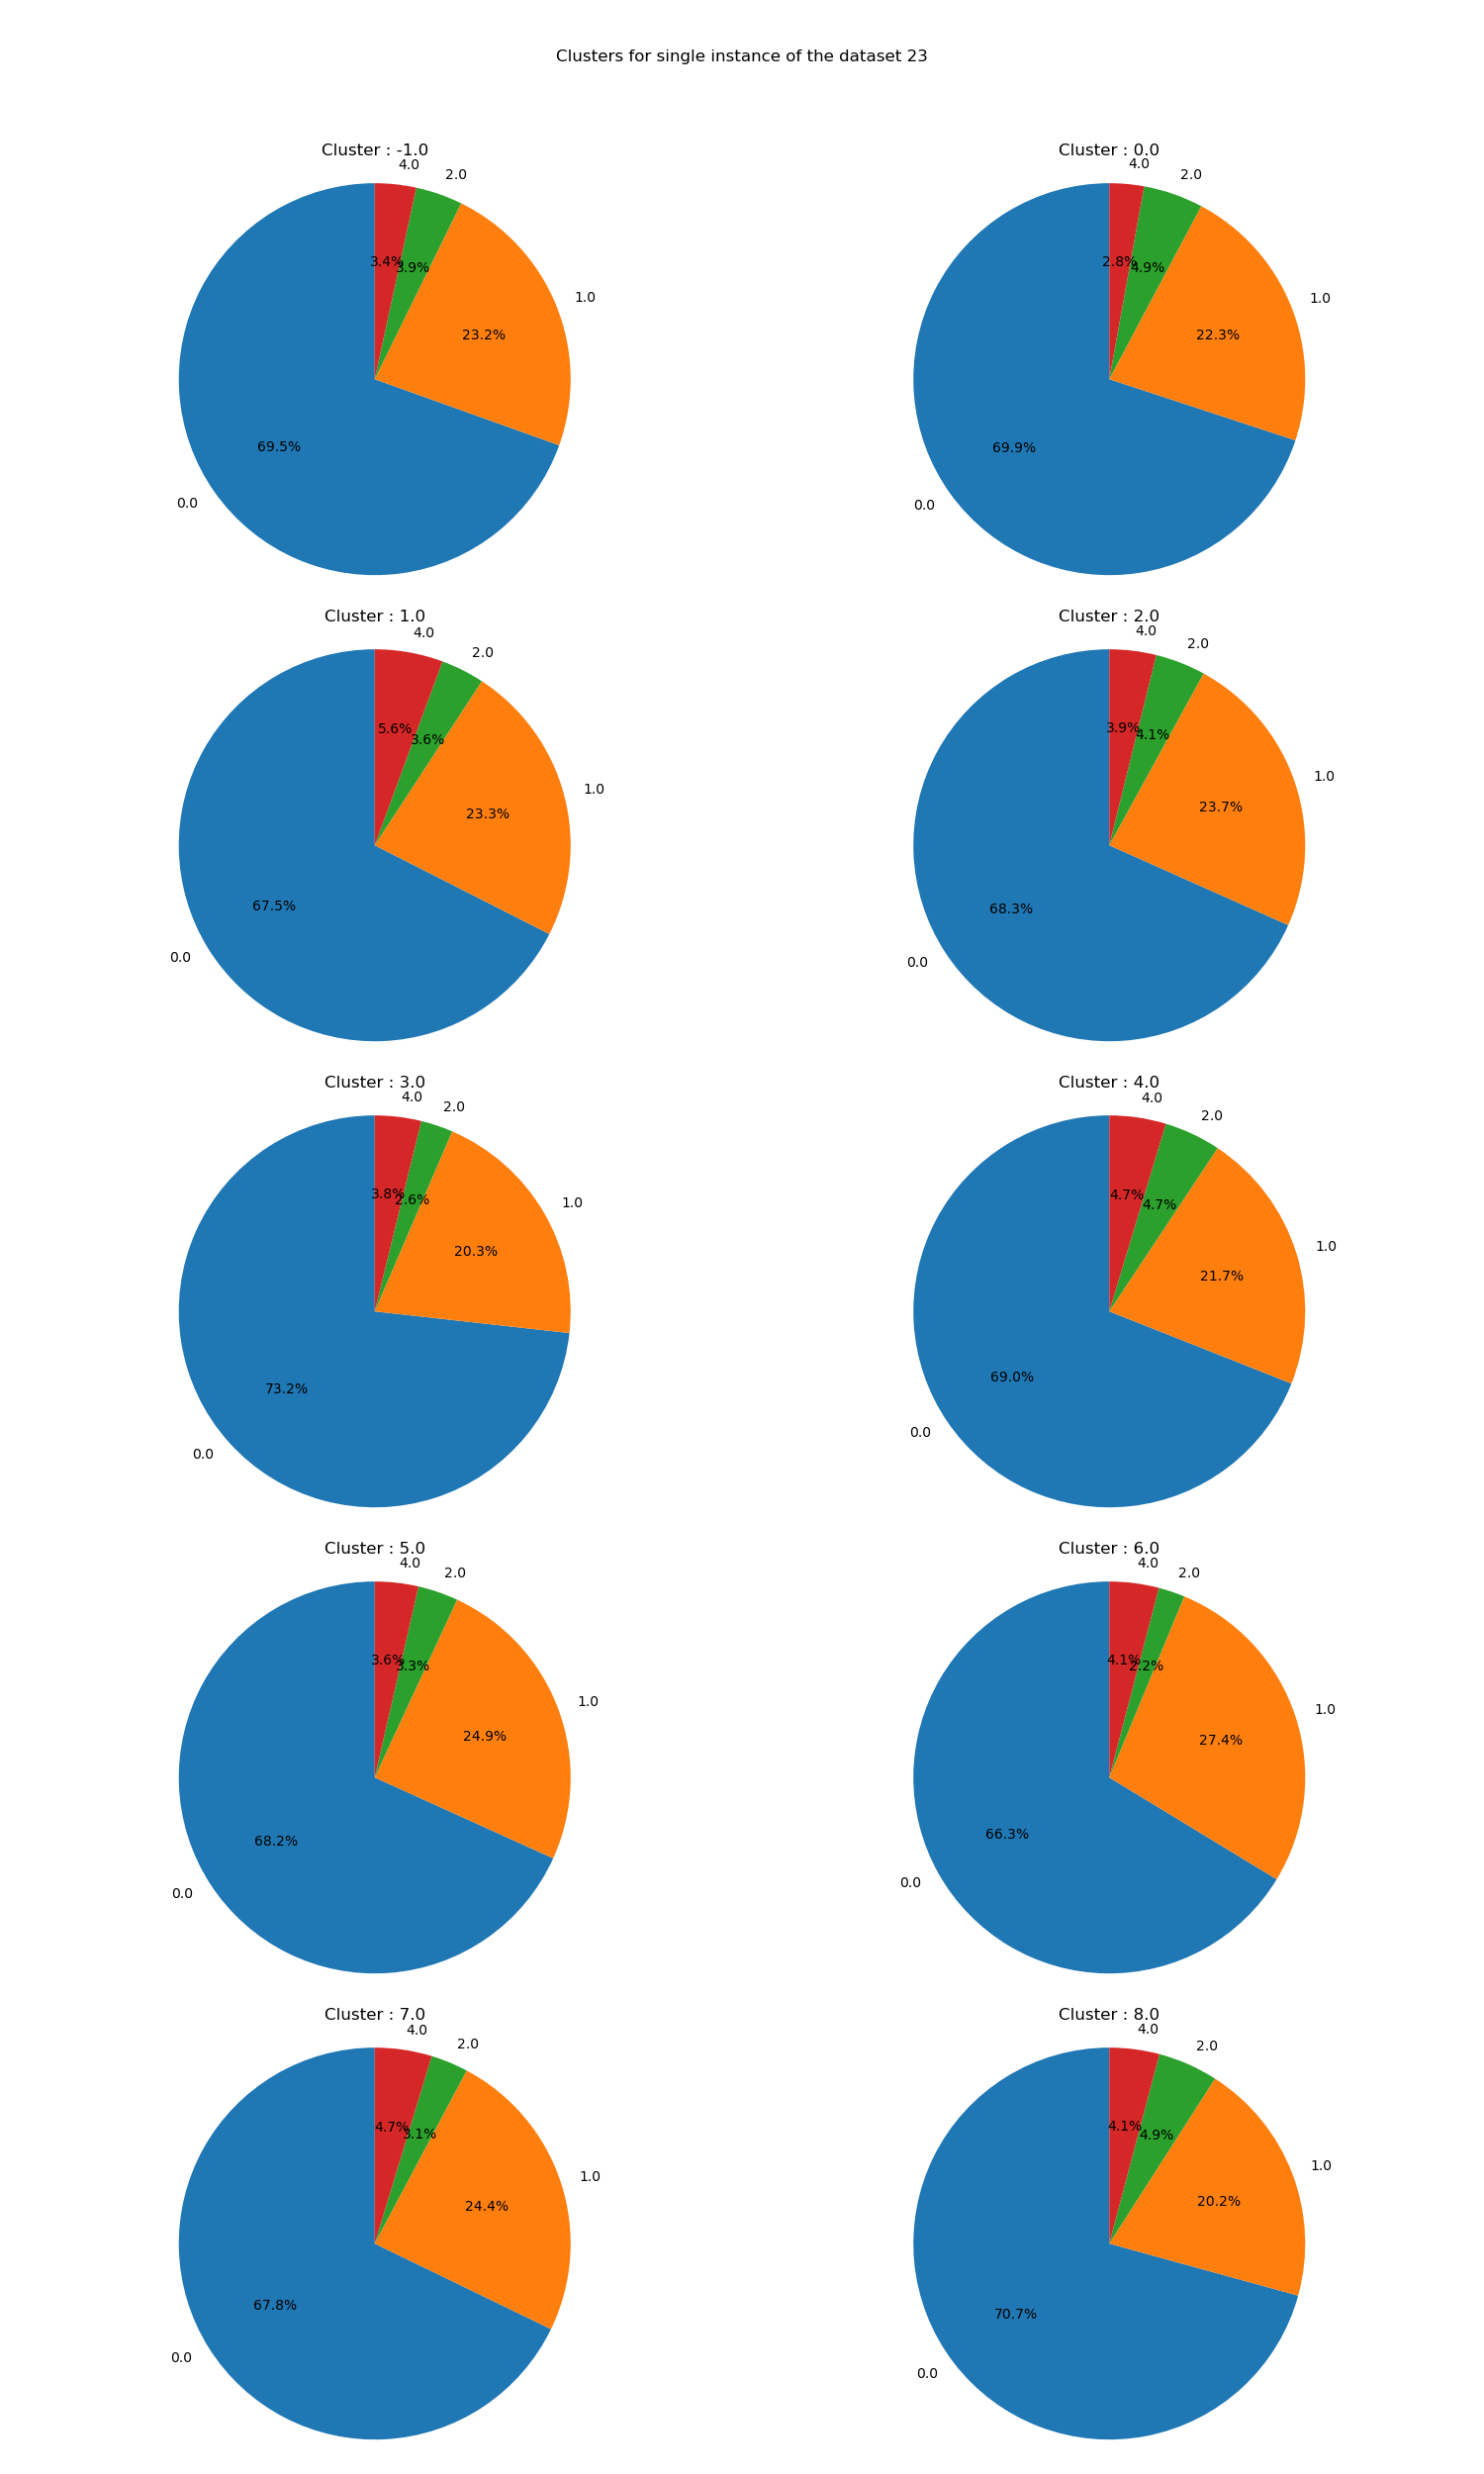
\includegraphics[width=0.8\linewidth]{img/annexes/23/clustering_pie_charts/single instance.png}} \\
\end{longtable}


\subsection{25 chunk\_extraction (filtered chunk size)}

\begin{longtable}{|c|c|c|c|c|}
\caption{Word2vec 3 Clustering Results on 25} \label{tab:25_word2vec_3_clustering_results}\\
\hline
\multicolumn{5}{|c|}{\textbf{General Information}} \\
\hline
\multicolumn{2}{|c|}{Min Samples} & \multicolumn{3}{c|}{937} \\
\multicolumn{2}{|c|}{Total Duration} & \multicolumn{3}{c|}{3634.492193 s} \\
\hline
\multicolumn{5}{|c|}{\textbf{Clustering Information}} \\
\hline
EPS & Number of Clusters & Silhouette Score & Noise Points & Duration \\
0.01 & 2 & 0.21665062010288239 & 3676 & 747.692523 s\\
0.02 & 1 & None & None & 697.073419 s\\
0.03 & 1 & None & None & 694.980969 s\\
0.04 & 1 & None & None & 737.728848 s\\
0.05 & 1 & None & None & 756.257249 s\\
\hline
\multicolumn{5}{|c|}{\textbf{Best EPS Information}} \\
\hline
0.01 & 2 & 0.21665062010288239 & 3676 & 747.692523 s\\
\hline
\multicolumn{5}{|c|}{\textbf{Label Association}} \\
\hline
Cluster ID & \multicolumn{2}{c|}{Label} & \multicolumn{2}{c|}{Number of Samples} \\
\hline
\multirow{4}{*}{-1.0} & \multicolumn{2}{c|}{0.0} & \multicolumn{2}{c|}{3} \\
& \multicolumn{2}{c|}{1.0} & \multicolumn{2}{c|}{2} \\
& \multicolumn{2}{c|}{2.0} & \multicolumn{2}{c|}{1} \\
& \multicolumn{2}{c|}{4.0} & \multicolumn{2}{c|}{2} \\
\hline
\multirow{2}{*}{0.0} & \multicolumn{2}{c|}{2.0} & \multicolumn{2}{c|}{2} \\
& \multicolumn{2}{c|}{4.0} & \multicolumn{2}{c|}{1} \\
\hline
\multirow{1}{*}{1.0} & \multicolumn{2}{c|}{0.0} & \multicolumn{2}{c|}{2} \\
\hline
\multicolumn{5}{|c|}{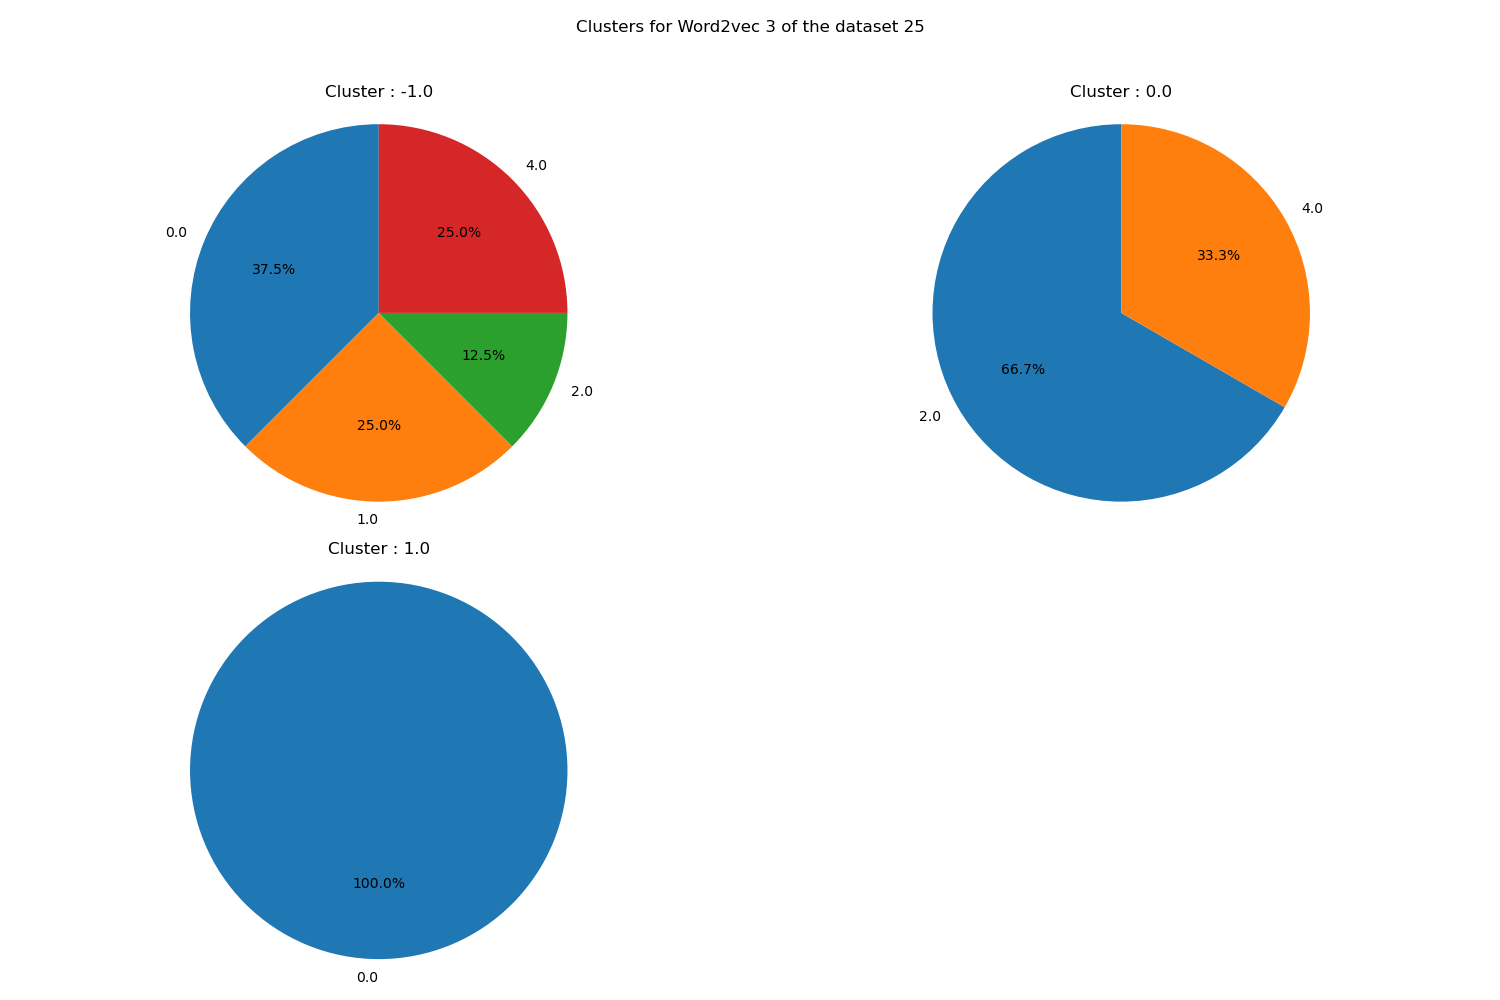
\includegraphics[width=0.8\linewidth]{img/annexes/25/clustering_pie_charts/Word2vec 3.png}} \\
\end{longtable}


\subsection{26 chunk\_extraction (filtered entropy)}

\begin{longtable}{|c|c|c|c|c|}
\caption{Transformers 0 Clustering Results on 26} \label{tab:26_transformers_0_clustering_results}\\
\hline
\multicolumn{5}{|c|}{\textbf{General Information}} \\
\hline
\multicolumn{2}{|c|}{Min Samples} & \multicolumn{3}{c|}{937} \\
\multicolumn{2}{|c|}{Total Duration} & \multicolumn{3}{c|}{3588.869441 s} \\
\hline
\multicolumn{5}{|c|}{\textbf{Clustering Information}} \\
\hline
EPS & Number of Clusters & Silhouette Score & Noise Points & Duration \\
0.01 & 3 & 0.5749053359031677 & 1369 & 674.16573 s\\
0.02 & 3 & 0.5749053359031677 & 1369 & 664.292675 s\\
0.03 & 3 & 0.574790894985199 & 1371 & 699.778419 s\\
0.04 & 3 & 0.574790894985199 & 1371 & 770.27842 s\\
0.05 & 3 & 0.574790894985199 & 1371 & 776.637103 s\\
\hline
\multicolumn{5}{|c|}{\textbf{Best EPS Information}} \\
\hline
0.01 & 3 & 0.5749053359031677 & 1369 & 674.16573 s\\
\hline
\multicolumn{5}{|c|}{\textbf{Label Association}} \\
\hline
Cluster ID & \multicolumn{2}{c|}{Label} & \multicolumn{2}{c|}{Number of Samples} \\
\hline
\multirow{4}{*}{-1.0} & \multicolumn{2}{c|}{0.0} & \multicolumn{2}{c|}{31} \\
& \multicolumn{2}{c|}{1.0} & \multicolumn{2}{c|}{40} \\
& \multicolumn{2}{c|}{2.0} & \multicolumn{2}{c|}{56} \\
& \multicolumn{2}{c|}{4.0} & \multicolumn{2}{c|}{33} \\
\hline
\multirow{4}{*}{0.0} & \multicolumn{2}{c|}{0.0} & \multicolumn{2}{c|}{35} \\
& \multicolumn{2}{c|}{1.0} & \multicolumn{2}{c|}{40} \\
& \multicolumn{2}{c|}{2.0} & \multicolumn{2}{c|}{26} \\
& \multicolumn{2}{c|}{4.0} & \multicolumn{2}{c|}{32} \\
\hline
\multirow{4}{*}{1.0} & \multicolumn{2}{c|}{0.0} & \multicolumn{2}{c|}{77} \\
& \multicolumn{2}{c|}{1.0} & \multicolumn{2}{c|}{91} \\
& \multicolumn{2}{c|}{2.0} & \multicolumn{2}{c|}{76} \\
& \multicolumn{2}{c|}{4.0} & \multicolumn{2}{c|}{96} \\
\hline
\multirow{4}{*}{2.0} & \multicolumn{2}{c|}{0.0} & \multicolumn{2}{c|}{32} \\
& \multicolumn{2}{c|}{1.0} & \multicolumn{2}{c|}{45} \\
& \multicolumn{2}{c|}{2.0} & \multicolumn{2}{c|}{45} \\
& \multicolumn{2}{c|}{4.0} & \multicolumn{2}{c|}{42} \\
\hline
\multicolumn{5}{|c|}{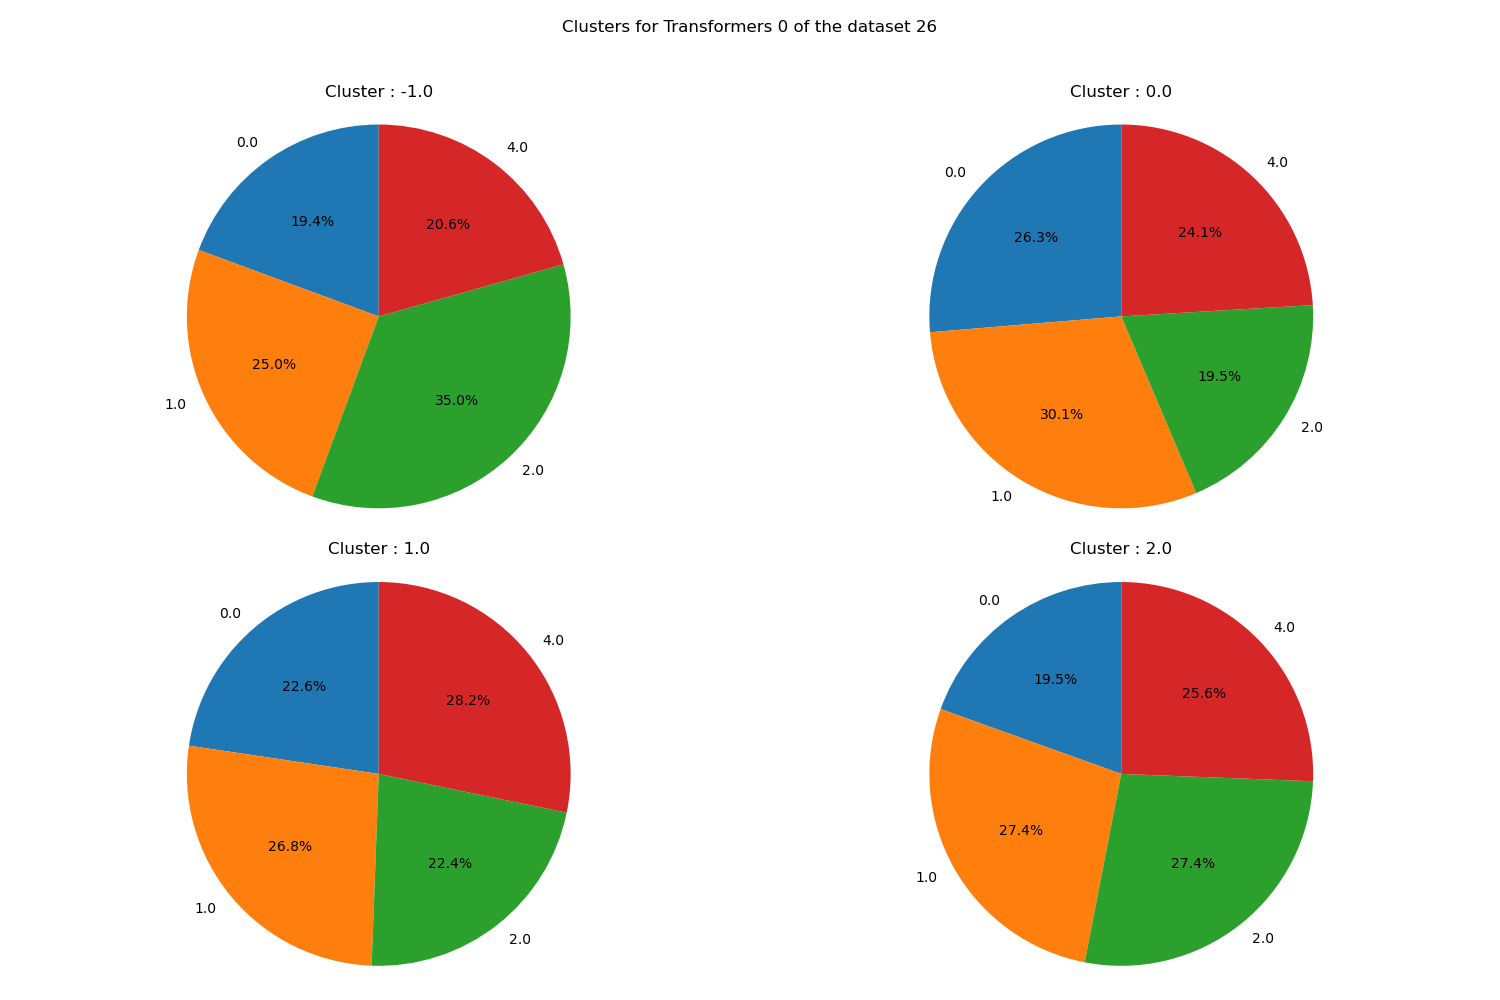
\includegraphics[width=0.8\linewidth]{img/annexes/26/clustering_pie_charts/Transformers 0.png}} \\
\end{longtable}


\begin{longtable}{|c|c|c|c|c|}
\caption{Transformers 1 Clustering Results on 26} \label{tab:26_transformers_1_clustering_results}\\
\hline
\multicolumn{5}{|c|}{\textbf{General Information}} \\
\hline
\multicolumn{2}{|c|}{Min Samples} & \multicolumn{3}{c|}{937} \\
\multicolumn{2}{|c|}{Total Duration} & \multicolumn{3}{c|}{3739.406415 s} \\
\hline
\multicolumn{5}{|c|}{\textbf{Clustering Information}} \\
\hline
EPS & Number of Clusters & Silhouette Score & Noise Points & Duration \\
0.01 & 3 & 0.7379494309425354 & 1299 & 760.134469 s\\
0.02 & 3 & 0.7379494309425354 & 1299 & 731.259721 s\\
0.03 & 3 & 0.7379494309425354 & 1299 & 738.923279 s\\
0.04 & 3 & 0.7379494309425354 & 1299 & 761.430407 s\\
0.05 & 3 & 0.3740614056587219 & 2696 & 743.313265 s\\
\hline
\multicolumn{5}{|c|}{\textbf{Best EPS Information}} \\
\hline
0.01 & 3 & 0.7379494309425354 & 1299 & 760.134469 s\\
\hline
\multicolumn{5}{|c|}{\textbf{Label Association}} \\
\hline
Cluster ID & \multicolumn{2}{c|}{Label} & \multicolumn{2}{c|}{Number of Samples} \\
\hline
\multirow{4}{*}{-1.0} & \multicolumn{2}{c|}{0.0} & \multicolumn{2}{c|}{29} \\
& \multicolumn{2}{c|}{1.0} & \multicolumn{2}{c|}{37} \\
& \multicolumn{2}{c|}{2.0} & \multicolumn{2}{c|}{56} \\
& \multicolumn{2}{c|}{4.0} & \multicolumn{2}{c|}{32} \\
\hline
\multirow{4}{*}{0.0} & \multicolumn{2}{c|}{0.0} & \multicolumn{2}{c|}{37} \\
& \multicolumn{2}{c|}{1.0} & \multicolumn{2}{c|}{43} \\
& \multicolumn{2}{c|}{2.0} & \multicolumn{2}{c|}{26} \\
& \multicolumn{2}{c|}{4.0} & \multicolumn{2}{c|}{33} \\
\hline
\multirow{4}{*}{1.0} & \multicolumn{2}{c|}{0.0} & \multicolumn{2}{c|}{77} \\
& \multicolumn{2}{c|}{1.0} & \multicolumn{2}{c|}{91} \\
& \multicolumn{2}{c|}{2.0} & \multicolumn{2}{c|}{76} \\
& \multicolumn{2}{c|}{4.0} & \multicolumn{2}{c|}{96} \\
\hline
\multirow{4}{*}{2.0} & \multicolumn{2}{c|}{0.0} & \multicolumn{2}{c|}{32} \\
& \multicolumn{2}{c|}{1.0} & \multicolumn{2}{c|}{45} \\
& \multicolumn{2}{c|}{2.0} & \multicolumn{2}{c|}{45} \\
& \multicolumn{2}{c|}{4.0} & \multicolumn{2}{c|}{42} \\
\hline
\multicolumn{5}{|c|}{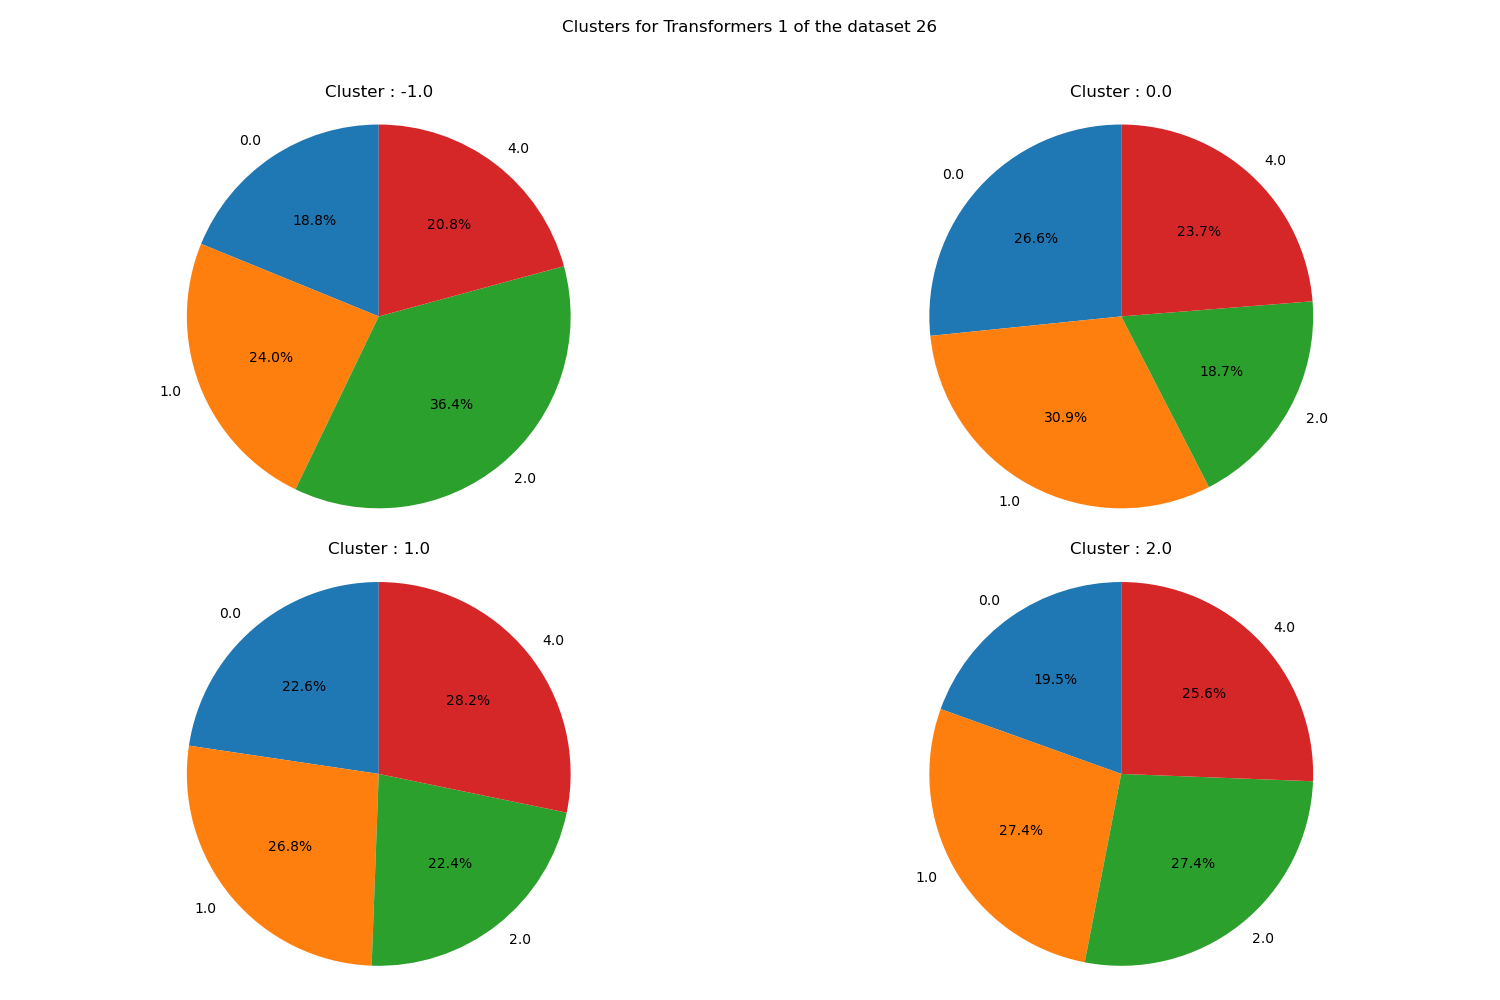
\includegraphics[width=0.8\linewidth]{img/annexes/26/clustering_pie_charts/Transformers 1.png}} \\
\end{longtable}


\subsection{27 chunk\_extraction (filtered entropy and chunk size)}

\begin{longtable}{|c|c|c|c|c|}
\caption{Transformers 0 Clustering Results on 27} \label{tab:27_transformers_0_clustering_results}\\
\hline
\multicolumn{5}{|c|}{\textbf{General Information}} \\
\hline
\multicolumn{2}{|c|}{Min Samples} & \multicolumn{3}{c|}{937} \\
\multicolumn{2}{|c|}{Total Duration} & \multicolumn{3}{c|}{3796.324605 s} \\
\hline
\multicolumn{5}{|c|}{\textbf{Clustering Information}} \\
\hline
EPS & Number of Clusters & Silhouette Score & Noise Points & Duration \\
0.01 & 3 & 0.2465989887714386 & 2274 & 709.617939 s\\
0.02 & 3 & 0.24514129757881165 & 2281 & 753.217155 s\\
0.03 & 2 & 0.1906411200761795 & 3242 & 820.552446 s\\
0.04 & 2 & 0.1906411200761795 & 3242 & 756.897654 s\\
0.05 & 2 & 0.1906411200761795 & 3242 & 751.836631 s\\
\hline
\multicolumn{5}{|c|}{\textbf{Best EPS Information}} \\
\hline
0.01 & 3 & 0.2465989887714386 & 2274 & 709.617939 s\\
\hline
\multicolumn{5}{|c|}{\textbf{Label Association}} \\
\hline
Cluster ID & \multicolumn{2}{c|}{Label} & \multicolumn{2}{c|}{Number of Samples} \\
\hline
\multirow{4}{*}{-1.0} & \multicolumn{2}{c|}{0.0} & \multicolumn{2}{c|}{91} \\
& \multicolumn{2}{c|}{1.0} & \multicolumn{2}{c|}{95} \\
& \multicolumn{2}{c|}{2.0} & \multicolumn{2}{c|}{99} \\
& \multicolumn{2}{c|}{4.0} & \multicolumn{2}{c|}{97} \\
\hline
\multirow{4}{*}{0.0} & \multicolumn{2}{c|}{0.0} & \multicolumn{2}{c|}{128} \\
& \multicolumn{2}{c|}{1.0} & \multicolumn{2}{c|}{129} \\
& \multicolumn{2}{c|}{2.0} & \multicolumn{2}{c|}{94} \\
& \multicolumn{2}{c|}{4.0} & \multicolumn{2}{c|}{110} \\
\hline
\multirow{4}{*}{1.0} & \multicolumn{2}{c|}{0.0} & \multicolumn{2}{c|}{50} \\
& \multicolumn{2}{c|}{1.0} & \multicolumn{2}{c|}{40} \\
& \multicolumn{2}{c|}{2.0} & \multicolumn{2}{c|}{44} \\
& \multicolumn{2}{c|}{4.0} & \multicolumn{2}{c|}{33} \\
\hline
\multirow{4}{*}{2.0} & \multicolumn{2}{c|}{0.0} & \multicolumn{2}{c|}{52} \\
& \multicolumn{2}{c|}{1.0} & \multicolumn{2}{c|}{51} \\
& \multicolumn{2}{c|}{2.0} & \multicolumn{2}{c|}{53} \\
& \multicolumn{2}{c|}{4.0} & \multicolumn{2}{c|}{50} \\
\hline
\multicolumn{5}{|c|}{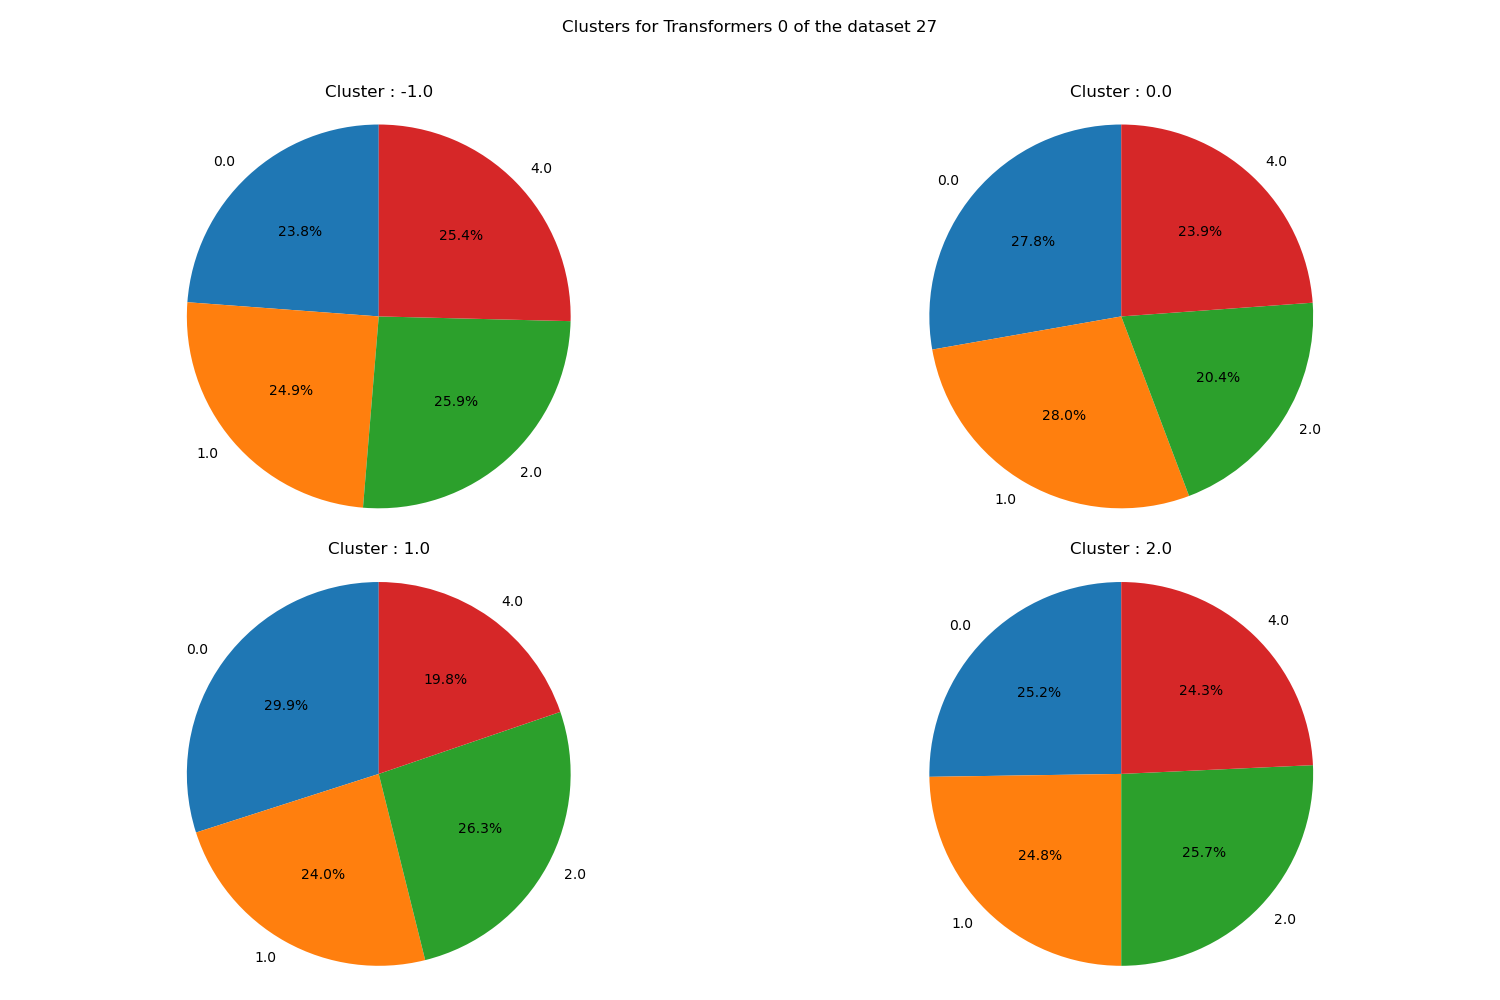
\includegraphics[width=0.8\linewidth]{img/annexes/27/clustering_pie_charts/Transformers 0.png}} \\
\end{longtable}


\begin{longtable}{|c|c|c|c|c|}
\caption{Transformers 1 Clustering Results on 27} \label{tab:27_transformers_1_clustering_results}\\
\hline
\multicolumn{5}{|c|}{\textbf{General Information}} \\
\hline
\multicolumn{2}{|c|}{Min Samples} & \multicolumn{3}{c|}{937} \\
\multicolumn{2}{|c|}{Total Duration} & \multicolumn{3}{c|}{3943.383724 s} \\
\hline
\multicolumn{5}{|c|}{\textbf{Clustering Information}} \\
\hline
EPS & Number of Clusters & Silhouette Score & Noise Points & Duration \\
0.01 & 4 & 0.5144023299217224 & 981 & 810.887225 s\\
0.02 & 3 & 0.8070926070213318 & 533 & 798.792131 s\\
0.03 & 3 & 0.8070926070213318 & 533 & 772.422919 s\\
0.04 & 3 & 0.8070926070213318 & 533 & 775.663572 s\\
0.05 & 3 & 0.8070926070213318 & 533 & 781.48437 s\\
\hline
\multicolumn{5}{|c|}{\textbf{Best EPS Information}} \\
\hline
0.02 & 3 & 0.8070926070213318 & 533 & 798.792131 s\\
\hline
\multicolumn{5}{|c|}{\textbf{Label Association}} \\
\hline
Cluster ID & \multicolumn{2}{c|}{Label} & \multicolumn{2}{c|}{Number of Samples} \\
\hline
\multirow{4}{*}{-1.0} & \multicolumn{2}{c|}{0.0} & \multicolumn{2}{c|}{19} \\
& \multicolumn{2}{c|}{1.0} & \multicolumn{2}{c|}{20} \\
& \multicolumn{2}{c|}{2.0} & \multicolumn{2}{c|}{20} \\
& \multicolumn{2}{c|}{4.0} & \multicolumn{2}{c|}{20} \\
\hline
\multirow{4}{*}{0.0} & \multicolumn{2}{c|}{0.0} & \multicolumn{2}{c|}{182} \\
& \multicolumn{2}{c|}{1.0} & \multicolumn{2}{c|}{155} \\
& \multicolumn{2}{c|}{2.0} & \multicolumn{2}{c|}{138} \\
& \multicolumn{2}{c|}{4.0} & \multicolumn{2}{c|}{145} \\
\hline
\multirow{4}{*}{1.0} & \multicolumn{2}{c|}{0.0} & \multicolumn{2}{c|}{74} \\
& \multicolumn{2}{c|}{1.0} & \multicolumn{2}{c|}{96} \\
& \multicolumn{2}{c|}{2.0} & \multicolumn{2}{c|}{81} \\
& \multicolumn{2}{c|}{4.0} & \multicolumn{2}{c|}{85} \\
\hline
\multirow{4}{*}{2.0} & \multicolumn{2}{c|}{0.0} & \multicolumn{2}{c|}{46} \\
& \multicolumn{2}{c|}{1.0} & \multicolumn{2}{c|}{44} \\
& \multicolumn{2}{c|}{2.0} & \multicolumn{2}{c|}{51} \\
& \multicolumn{2}{c|}{4.0} & \multicolumn{2}{c|}{40} \\
\hline
\multicolumn{5}{|c|}{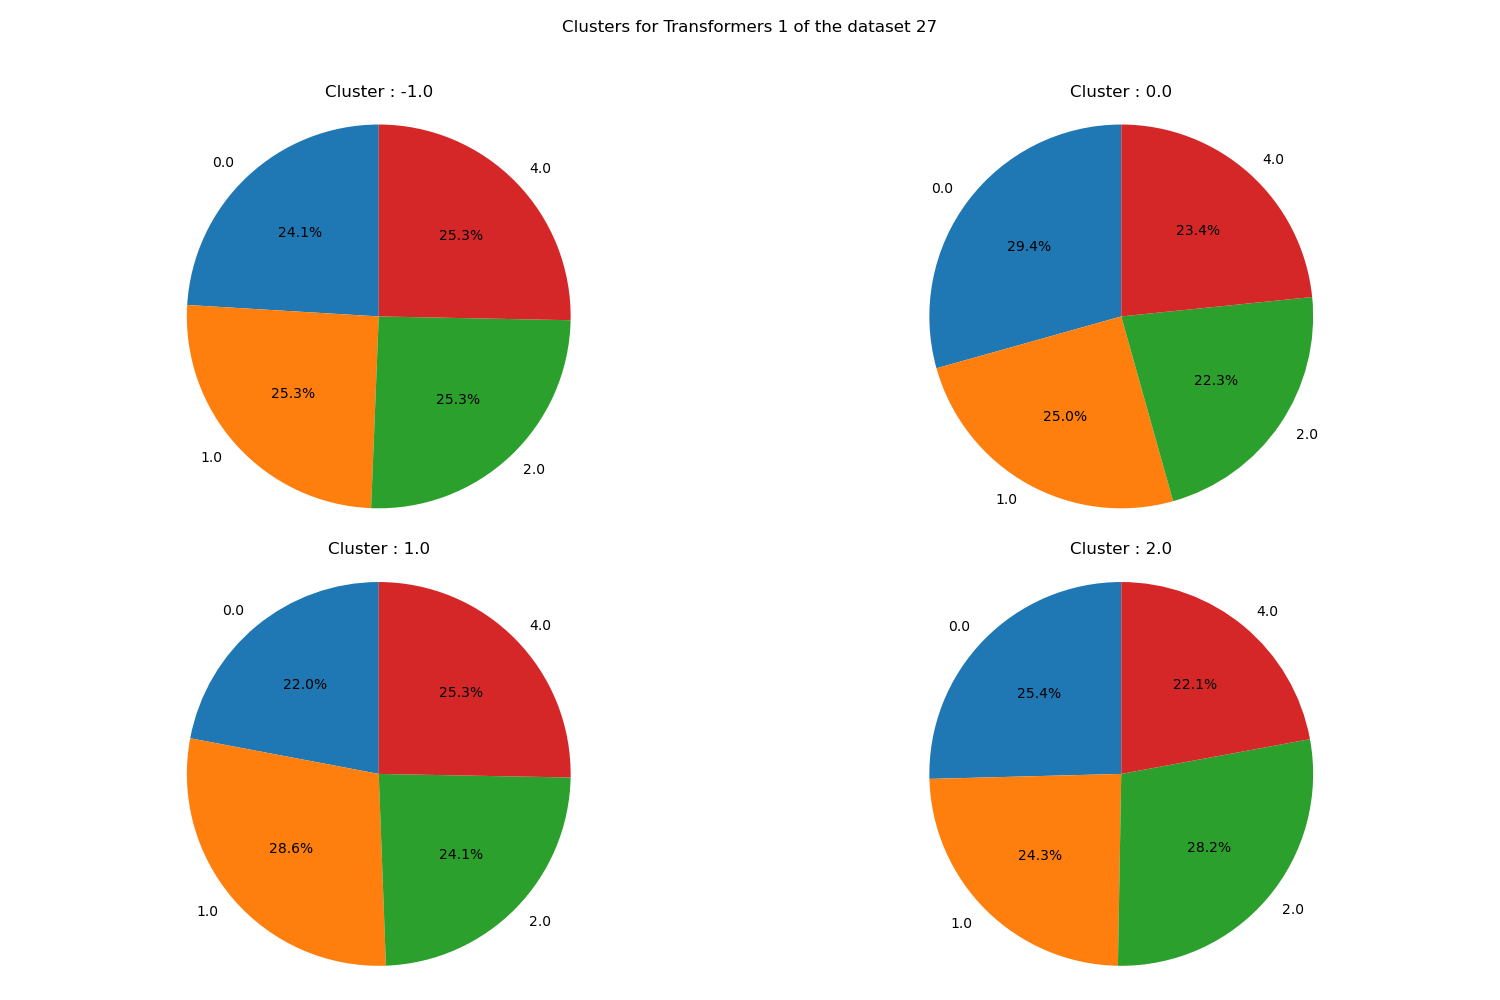
\includegraphics[width=0.8\linewidth]{img/annexes/27/clustering_pie_charts/Transformers 1.png}} \\
\end{longtable}


\begin{longtable}{|c|c|c|c|c|}
\caption{Transformers 2 Clustering Results on 27} \label{tab:27_transformers_2_clustering_results}\\
\hline
\multicolumn{5}{|c|}{\textbf{General Information}} \\
\hline
\multicolumn{2}{|c|}{Min Samples} & \multicolumn{3}{c|}{937} \\
\multicolumn{2}{|c|}{Total Duration} & \multicolumn{3}{c|}{3895.618311 s} \\
\hline
\multicolumn{5}{|c|}{\textbf{Clustering Information}} \\
\hline
EPS & Number of Clusters & Silhouette Score & Noise Points & Duration \\
0.01 & 2 & 0.907838761806488 & 0 & 790.283896 s\\
0.02 & 2 & 0.907838761806488 & 0 & 802.295121 s\\
0.03 & 2 & 0.907838761806488 & 0 & 787.142639 s\\
0.04 & 2 & 0.907838761806488 & 0 & 725.182204 s\\
0.05 & 2 & 0.907838761806488 & 0 & 785.995246 s\\
\hline
\multicolumn{5}{|c|}{\textbf{Best EPS Information}} \\
\hline
0.01 & 2 & 0.907838761806488 & 0 & 790.283896 s\\
\hline
\multicolumn{5}{|c|}{\textbf{Label Association}} \\
\hline
Cluster ID & \multicolumn{2}{c|}{Label} & \multicolumn{2}{c|}{Number of Samples} \\
\hline
\multirow{4}{*}{0.0} & \multicolumn{2}{c|}{0.0} & \multicolumn{2}{c|}{264} \\
& \multicolumn{2}{c|}{1.0} & \multicolumn{2}{c|}{256} \\
& \multicolumn{2}{c|}{2.0} & \multicolumn{2}{c|}{228} \\
& \multicolumn{2}{c|}{4.0} & \multicolumn{2}{c|}{236} \\
\hline
\multirow{4}{*}{1.0} & \multicolumn{2}{c|}{0.0} & \multicolumn{2}{c|}{57} \\
& \multicolumn{2}{c|}{1.0} & \multicolumn{2}{c|}{59} \\
& \multicolumn{2}{c|}{2.0} & \multicolumn{2}{c|}{62} \\
& \multicolumn{2}{c|}{4.0} & \multicolumn{2}{c|}{54} \\
\hline
\multicolumn{5}{|c|}{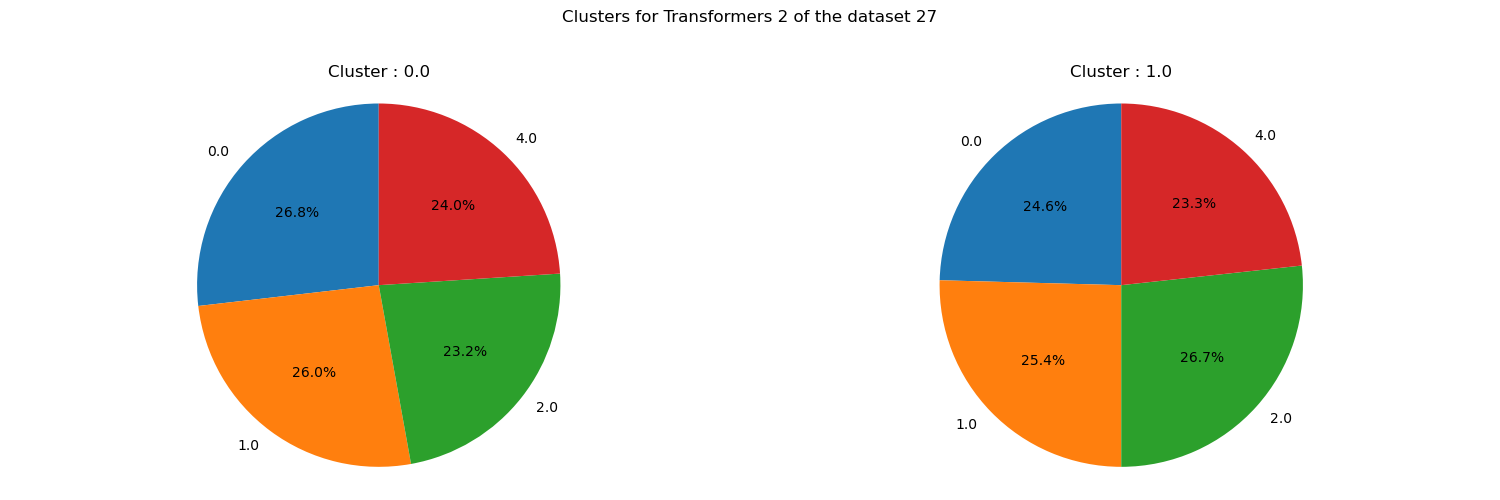
\includegraphics[width=0.8\linewidth]{img/annexes/27/clustering_pie_charts/Transformers 2.png}} \\
\end{longtable}


\begin{longtable}{|c|c|c|c|c|}
\caption{Transformers 3 Clustering Results on 27} \label{tab:27_transformers_3_clustering_results}\\
\hline
\multicolumn{5}{|c|}{\textbf{General Information}} \\
\hline
\multicolumn{2}{|c|}{Min Samples} & \multicolumn{3}{c|}{937} \\
\multicolumn{2}{|c|}{Total Duration} & \multicolumn{3}{c|}{3939.333846 s} \\
\hline
\multicolumn{5}{|c|}{\textbf{Clustering Information}} \\
\hline
EPS & Number of Clusters & Silhouette Score & Noise Points & Duration \\
0.01 & 3 & 0.36908280849456787 & 2637 & 806.707338 s\\
0.02 & 3 & 0.36908280849456787 & 2637 & 782.581847 s\\
0.03 & 3 & 0.36908280849456787 & 2637 & 775.659231 s\\
0.04 & 3 & 0.36908280849456787 & 2637 & 783.727976 s\\
0.05 & 3 & 0.36908280849456787 & 2637 & 786.255646 s\\
\hline
\multicolumn{5}{|c|}{\textbf{Best EPS Information}} \\
\hline
0.01 & 3 & 0.36908280849456787 & 2637 & 806.707338 s\\
\hline
\multicolumn{5}{|c|}{\textbf{Label Association}} \\
\hline
Cluster ID & \multicolumn{2}{c|}{Label} & \multicolumn{2}{c|}{Number of Samples} \\
\hline
\multirow{4}{*}{-1.0} & \multicolumn{2}{c|}{0.0} & \multicolumn{2}{c|}{134} \\
& \multicolumn{2}{c|}{1.0} & \multicolumn{2}{c|}{97} \\
& \multicolumn{2}{c|}{2.0} & \multicolumn{2}{c|}{114} \\
& \multicolumn{2}{c|}{4.0} & \multicolumn{2}{c|}{111} \\
\hline
\multirow{4}{*}{0.0} & \multicolumn{2}{c|}{0.0} & \multicolumn{2}{c|}{81} \\
& \multicolumn{2}{c|}{1.0} & \multicolumn{2}{c|}{86} \\
& \multicolumn{2}{c|}{2.0} & \multicolumn{2}{c|}{53} \\
& \multicolumn{2}{c|}{4.0} & \multicolumn{2}{c|}{72} \\
\hline
\multirow{4}{*}{1.0} & \multicolumn{2}{c|}{0.0} & \multicolumn{2}{c|}{49} \\
& \multicolumn{2}{c|}{1.0} & \multicolumn{2}{c|}{73} \\
& \multicolumn{2}{c|}{2.0} & \multicolumn{2}{c|}{61} \\
& \multicolumn{2}{c|}{4.0} & \multicolumn{2}{c|}{53} \\
\hline
\multirow{4}{*}{2.0} & \multicolumn{2}{c|}{0.0} & \multicolumn{2}{c|}{57} \\
& \multicolumn{2}{c|}{1.0} & \multicolumn{2}{c|}{59} \\
& \multicolumn{2}{c|}{2.0} & \multicolumn{2}{c|}{62} \\
& \multicolumn{2}{c|}{4.0} & \multicolumn{2}{c|}{54} \\
\hline
\multicolumn{5}{|c|}{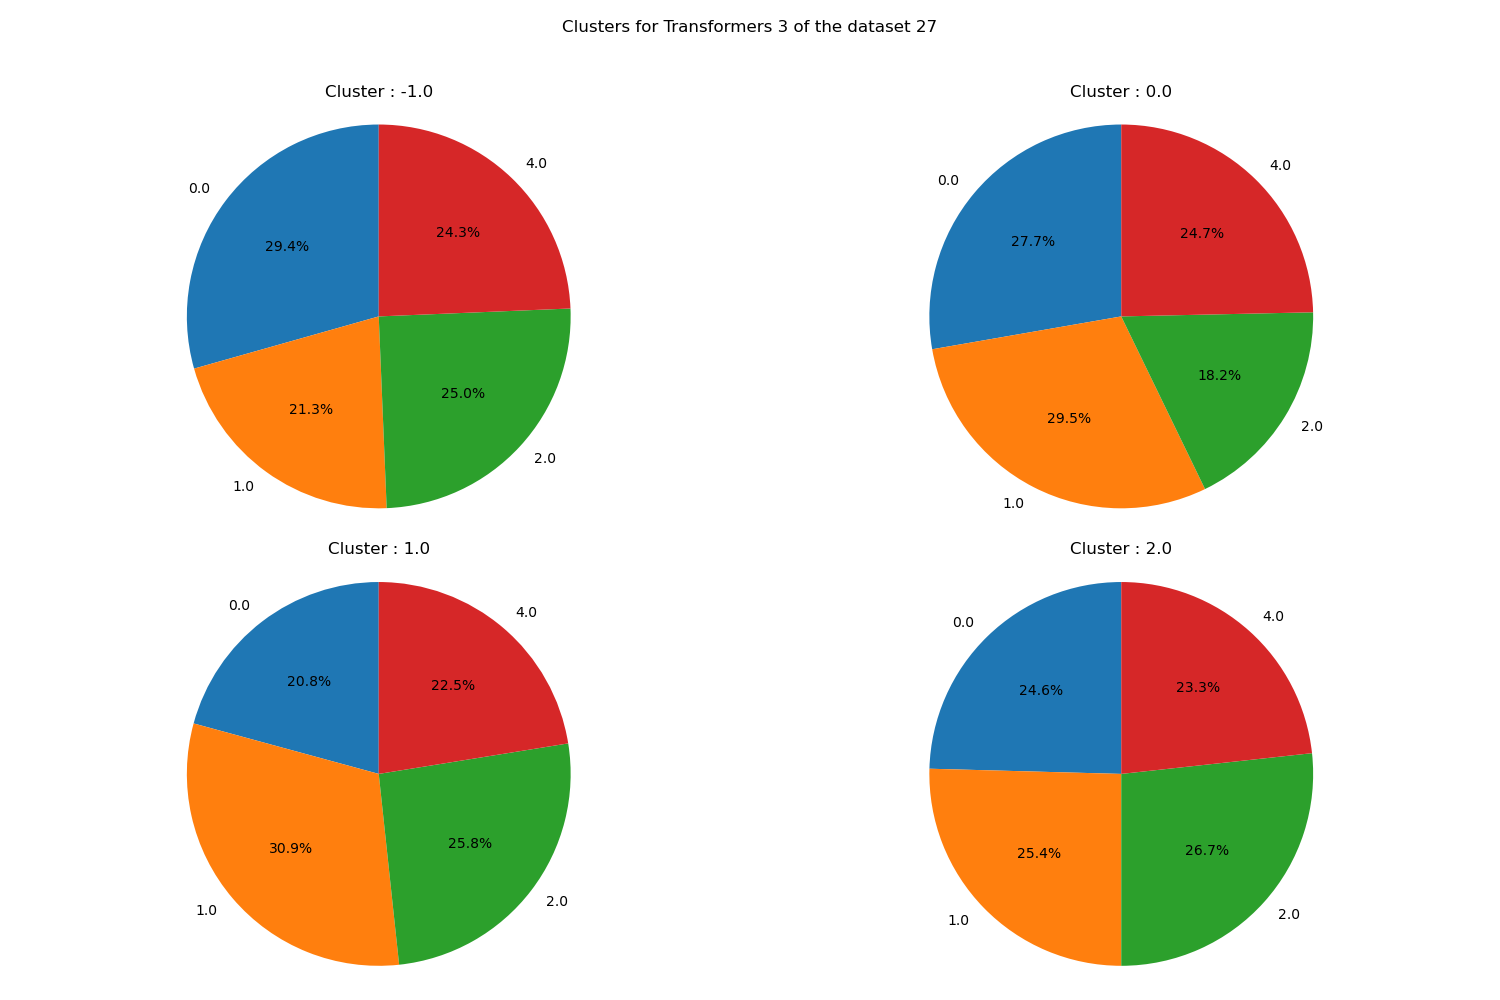
\includegraphics[width=0.8\linewidth]{img/annexes/27/clustering_pie_charts/Transformers 3.png}} \\
\end{longtable}


\begin{longtable}{|c|c|c|c|c|}
\caption{Transformers 4 Clustering Results on 27} \label{tab:27_transformers_4_clustering_results}\\
\hline
\multicolumn{5}{|c|}{\textbf{General Information}} \\
\hline
\multicolumn{2}{|c|}{Min Samples} & \multicolumn{3}{c|}{937} \\
\multicolumn{2}{|c|}{Total Duration} & \multicolumn{3}{c|}{3803.240679 s} \\
\hline
\multicolumn{5}{|c|}{\textbf{Clustering Information}} \\
\hline
EPS & Number of Clusters & Silhouette Score & Noise Points & Duration \\
0.01 & 3 & 0.6185895800590515 & 1103 & 794.276663 s\\
0.02 & 3 & 0.6185895800590515 & 1103 & 746.079328 s\\
0.03 & 3 & 0.6186758875846863 & 1105 & 737.198024 s\\
0.04 & 2 & 0.47322237491607666 & 2390 & 732.879635 s\\
0.05 & 2 & 0.47322237491607666 & 2390 & 788.087243 s\\
\hline
\multicolumn{5}{|c|}{\textbf{Best EPS Information}} \\
\hline
0.03 & 3 & 0.6186758875846863 & 1105 & 737.198024 s\\
\hline
\multicolumn{5}{|c|}{\textbf{Label Association}} \\
\hline
Cluster ID & \multicolumn{2}{c|}{Label} & \multicolumn{2}{c|}{Number of Samples} \\
\hline
\multirow{4}{*}{-1.0} & \multicolumn{2}{c|}{0.0} & \multicolumn{2}{c|}{44} \\
& \multicolumn{2}{c|}{1.0} & \multicolumn{2}{c|}{43} \\
& \multicolumn{2}{c|}{2.0} & \multicolumn{2}{c|}{43} \\
& \multicolumn{2}{c|}{4.0} & \multicolumn{2}{c|}{53} \\
\hline
\multirow{4}{*}{0.0} & \multicolumn{2}{c|}{0.0} & \multicolumn{2}{c|}{184} \\
& \multicolumn{2}{c|}{1.0} & \multicolumn{2}{c|}{159} \\
& \multicolumn{2}{c|}{2.0} & \multicolumn{2}{c|}{140} \\
& \multicolumn{2}{c|}{4.0} & \multicolumn{2}{c|}{146} \\
\hline
\multirow{4}{*}{1.0} & \multicolumn{2}{c|}{0.0} & \multicolumn{2}{c|}{47} \\
& \multicolumn{2}{c|}{1.0} & \multicolumn{2}{c|}{69} \\
& \multicolumn{2}{c|}{2.0} & \multicolumn{2}{c|}{59} \\
& \multicolumn{2}{c|}{4.0} & \multicolumn{2}{c|}{52} \\
\hline
\multirow{4}{*}{2.0} & \multicolumn{2}{c|}{0.0} & \multicolumn{2}{c|}{46} \\
& \multicolumn{2}{c|}{1.0} & \multicolumn{2}{c|}{44} \\
& \multicolumn{2}{c|}{2.0} & \multicolumn{2}{c|}{48} \\
& \multicolumn{2}{c|}{4.0} & \multicolumn{2}{c|}{39} \\
\hline
\multicolumn{5}{|c|}{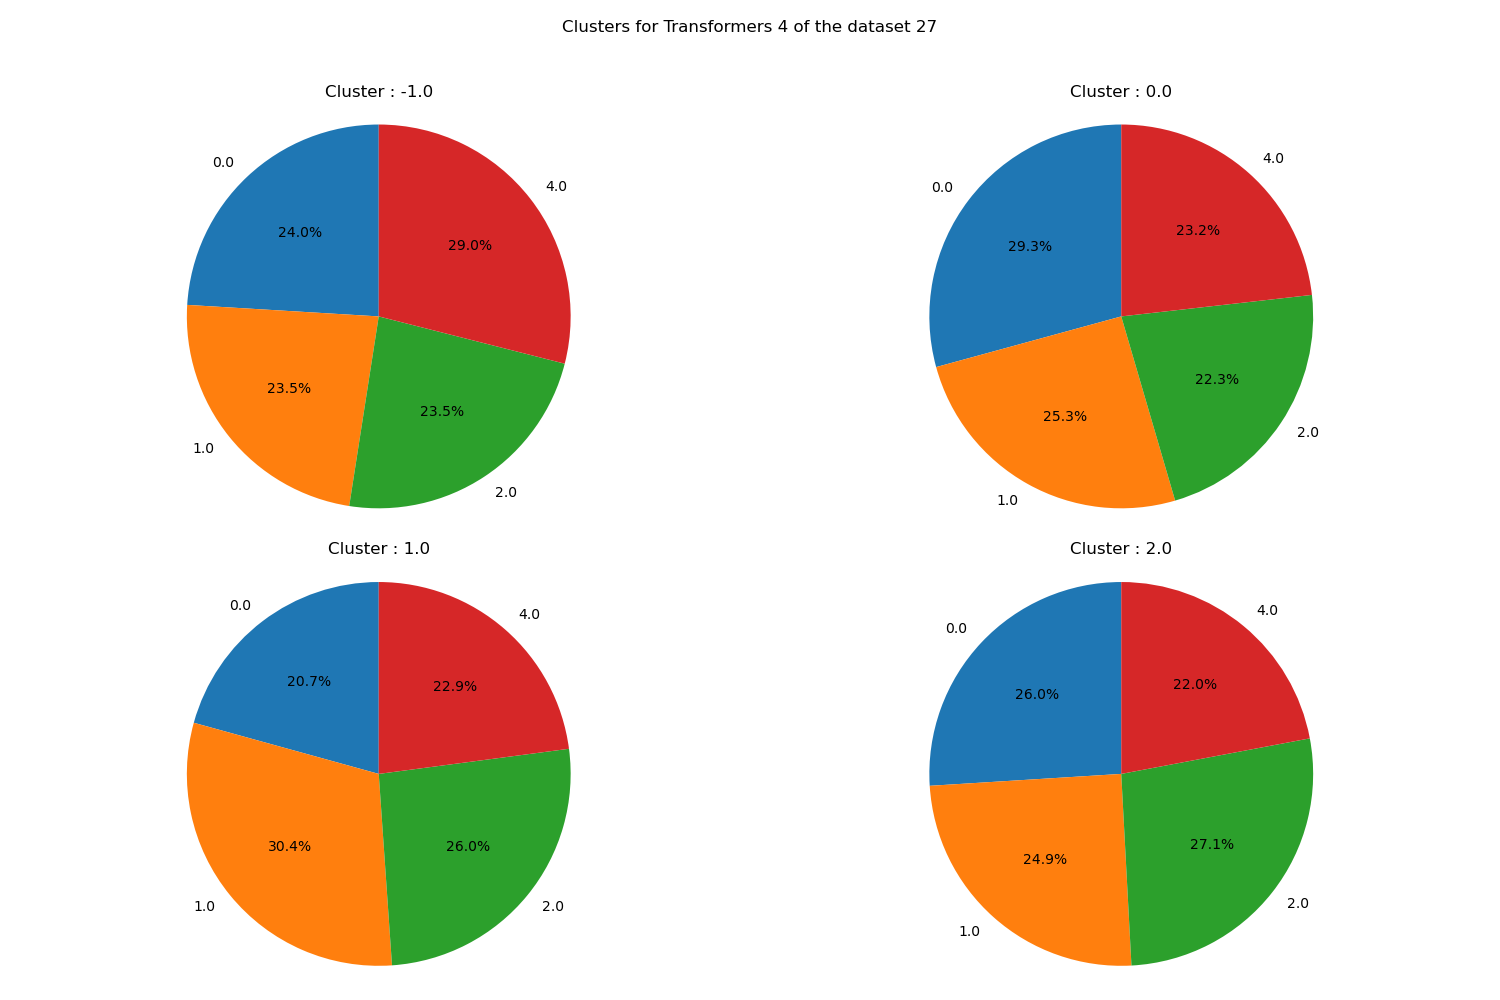
\includegraphics[width=0.8\linewidth]{img/annexes/27/clustering_pie_charts/Transformers 4.png}} \\
\end{longtable}


\begin{longtable}{|c|c|c|c|c|}
\caption{Transformers 6 Clustering Results on 27} \label{tab:27_transformers_6_clustering_results}\\
\hline
\multicolumn{5}{|c|}{\textbf{General Information}} \\
\hline
\multicolumn{2}{|c|}{Min Samples} & \multicolumn{3}{c|}{937} \\
\multicolumn{2}{|c|}{Total Duration} & \multicolumn{3}{c|}{3973.074733 s} \\
\hline
\multicolumn{5}{|c|}{\textbf{Clustering Information}} \\
\hline
EPS & Number of Clusters & Silhouette Score & Noise Points & Duration \\
0.01 & 3 & 0.37613049149513245 & 2636 & 806.924699 s\\
0.02 & 3 & 0.37613049149513245 & 2636 & 759.43715 s\\
0.03 & 3 & 0.37613049149513245 & 2636 & 762.661041 s\\
0.04 & 3 & 0.37613049149513245 & 2636 & 821.687468 s\\
0.05 & 3 & 0.37613049149513245 & 2636 & 818.360119 s\\
\hline
\multicolumn{5}{|c|}{\textbf{Best EPS Information}} \\
\hline
0.01 & 3 & 0.37613049149513245 & 2636 & 806.924699 s\\
\hline
\multicolumn{5}{|c|}{\textbf{Label Association}} \\
\hline
Cluster ID & \multicolumn{2}{c|}{Label} & \multicolumn{2}{c|}{Number of Samples} \\
\hline
\multirow{4}{*}{-1.0} & \multicolumn{2}{c|}{0.0} & \multicolumn{2}{c|}{134} \\
& \multicolumn{2}{c|}{1.0} & \multicolumn{2}{c|}{97} \\
& \multicolumn{2}{c|}{2.0} & \multicolumn{2}{c|}{114} \\
& \multicolumn{2}{c|}{4.0} & \multicolumn{2}{c|}{111} \\
\hline
\multirow{4}{*}{0.0} & \multicolumn{2}{c|}{0.0} & \multicolumn{2}{c|}{81} \\
& \multicolumn{2}{c|}{1.0} & \multicolumn{2}{c|}{86} \\
& \multicolumn{2}{c|}{2.0} & \multicolumn{2}{c|}{53} \\
& \multicolumn{2}{c|}{4.0} & \multicolumn{2}{c|}{72} \\
\hline
\multirow{4}{*}{1.0} & \multicolumn{2}{c|}{0.0} & \multicolumn{2}{c|}{49} \\
& \multicolumn{2}{c|}{1.0} & \multicolumn{2}{c|}{73} \\
& \multicolumn{2}{c|}{2.0} & \multicolumn{2}{c|}{61} \\
& \multicolumn{2}{c|}{4.0} & \multicolumn{2}{c|}{53} \\
\hline
\multirow{4}{*}{2.0} & \multicolumn{2}{c|}{0.0} & \multicolumn{2}{c|}{57} \\
& \multicolumn{2}{c|}{1.0} & \multicolumn{2}{c|}{59} \\
& \multicolumn{2}{c|}{2.0} & \multicolumn{2}{c|}{62} \\
& \multicolumn{2}{c|}{4.0} & \multicolumn{2}{c|}{54} \\
\hline
\multicolumn{5}{|c|}{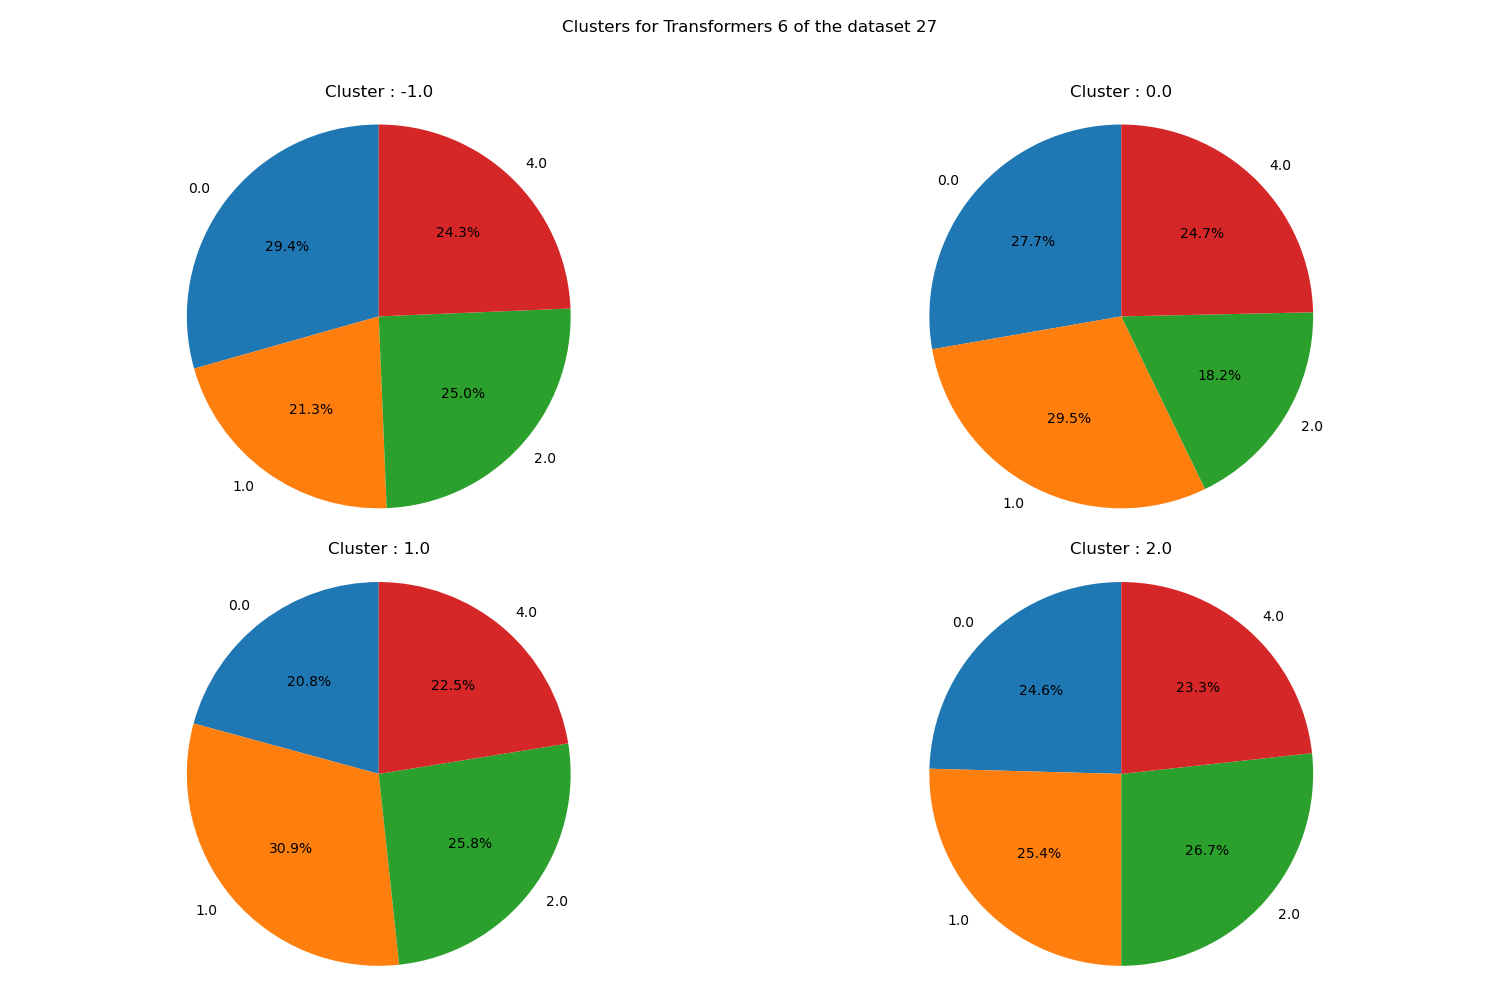
\includegraphics[width=0.8\linewidth]{img/annexes/27/clustering_pie_charts/Transformers 6.png}} \\
\end{longtable}


\begin{longtable}{|c|c|c|c|c|}
\caption{Word2vec 1 Clustering Results on 27} \label{tab:27_word2vec_1_clustering_results}\\
\hline
\multicolumn{5}{|c|}{\textbf{General Information}} \\
\hline
\multicolumn{2}{|c|}{Min Samples} & \multicolumn{3}{c|}{937} \\
\multicolumn{2}{|c|}{Total Duration} & \multicolumn{3}{c|}{4102.458592 s} \\
\hline
\multicolumn{5}{|c|}{\textbf{Clustering Information}} \\
\hline
EPS & Number of Clusters & Silhouette Score & Noise Points & Duration \\
0.01 & 2 & 0.2816171944141388 & 3355 & 861.723101 s\\
0.02 & 2 & 0.24786975979804993 & 3822 & 806.529987 s\\
0.03 & 2 & 0.23544950783252716 & 3938 & 786.201026 s\\
0.04 & 2 & 0.2358776181936264 & 3952 & 838.073615 s\\
0.05 & 2 & 0.2358776181936264 & 3952 & 805.644238 s\\
\hline
\multicolumn{5}{|c|}{\textbf{Best EPS Information}} \\
\hline
0.01 & 2 & 0.2816171944141388 & 3355 & 861.723101 s\\
\hline
\multicolumn{5}{|c|}{\textbf{Label Association}} \\
\hline
Cluster ID & \multicolumn{2}{c|}{Label} & \multicolumn{2}{c|}{Number of Samples} \\
\hline
\multirow{4}{*}{-1.0} & \multicolumn{2}{c|}{0.0} & \multicolumn{2}{c|}{149} \\
& \multicolumn{2}{c|}{1.0} & \multicolumn{2}{c|}{140} \\
& \multicolumn{2}{c|}{2.0} & \multicolumn{2}{c|}{126} \\
& \multicolumn{2}{c|}{4.0} & \multicolumn{2}{c|}{135} \\
\hline
\multirow{4}{*}{0.0} & \multicolumn{2}{c|}{0.0} & \multicolumn{2}{c|}{60} \\
& \multicolumn{2}{c|}{1.0} & \multicolumn{2}{c|}{66} \\
& \multicolumn{2}{c|}{2.0} & \multicolumn{2}{c|}{63} \\
& \multicolumn{2}{c|}{4.0} & \multicolumn{2}{c|}{72} \\
\hline
\multirow{4}{*}{1.0} & \multicolumn{2}{c|}{0.0} & \multicolumn{2}{c|}{112} \\
& \multicolumn{2}{c|}{1.0} & \multicolumn{2}{c|}{109} \\
& \multicolumn{2}{c|}{2.0} & \multicolumn{2}{c|}{101} \\
& \multicolumn{2}{c|}{4.0} & \multicolumn{2}{c|}{83} \\
\hline
\multicolumn{5}{|c|}{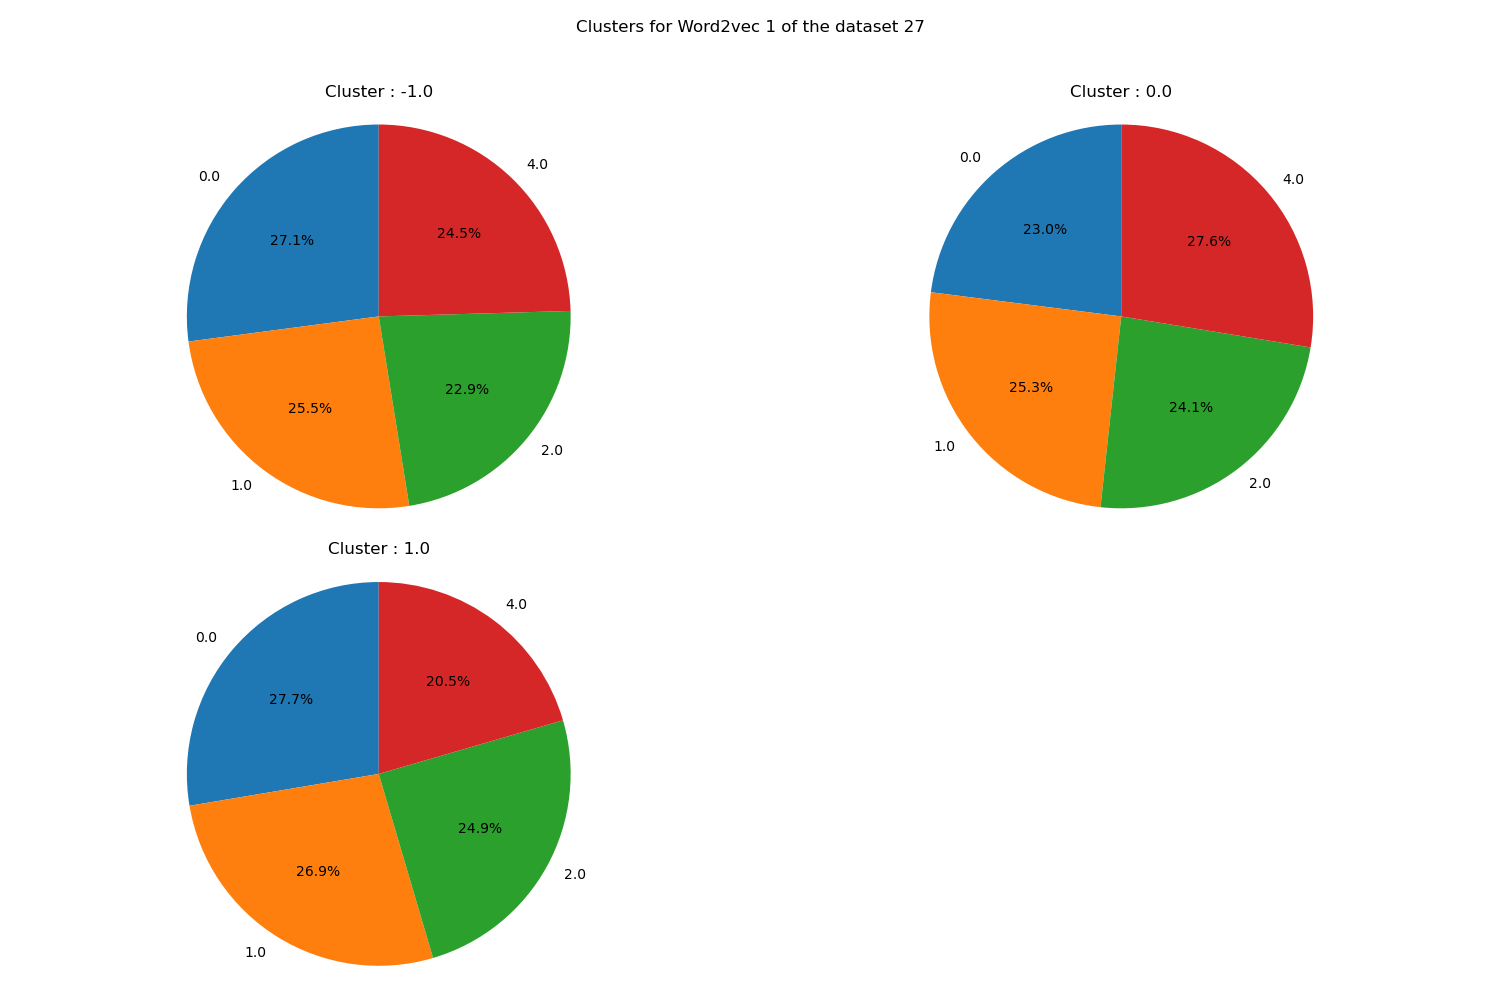
\includegraphics[width=0.8\linewidth]{img/annexes/27/clustering_pie_charts/Word2vec 1.png}} \\
\end{longtable}


\section{Classification results}

\label{sec:annexe:classification_results}

\subsection{8 chunk\_semantic\_embedding}

\begin{longtable}{|c|c|c|}
\caption{single instance Classification Results on 8} \label{tab:8_single_instance_classifiers_results} \\
\hline
Class & Metric Name & Metric Value \\
\hline
\multirow{4}{*}{0.0} & Precision & 0.9999964810195971 \\
 & Recall & 0.9846863570570408 \\
 & F1 Score & 0.9922823668080956 \\
 & Support & 5194649.0 \\
 & Final Samples (after rebalancing) & 20964 \\
 & Initial Samples (before rebalancing) & 28781019 \\
\hline
\multirow{4}{*}{1.0} & Precision & 0.21965646795695548 \\
 & Recall & 0.9991967871485944 \\
 & F1 Score & 0.3601418565190469 \\
 & Support & 22410.0 \\
 & Final Samples (after rebalancing) & 20964 \\
 & Initial Samples (before rebalancing) & 125784 \\
\hline
\multirow{4}{*}{2.0} & Precision & 1.0 \\
 & Recall & 1.0 \\
 & F1 Score & 1.0 \\
 & Support & 3735.0 \\
 & Final Samples (after rebalancing) & 20964 \\
 & Initial Samples (before rebalancing) & 20964 \\
\hline
\multirow{4}{*}{4.0} & Precision & 1.0 \\
 & Recall & 1.0 \\
 & F1 Score & 1.0 \\
 & Support & 3735.0 \\
 & Final Samples (after rebalancing) & 20964 \\
 & Initial Samples (before rebalancing) & 20964 \\
\hline
\multirow{4}{*}{Macro Avg} & Precision & 0.8049132372441381 \\
 & Recall & 0.9959707860514088 \\
 & F1 Score & 0.8381060558317857 \\
 & Support & 5224529.0 \\
 & Final Samples (after rebalancing) & 83856 \\
 & Initial Samples (before rebalancing) & 28948731 \\
\hline
\multirow{4}{*}{Weighted Avg} & Precision & 0.996649309742349 \\
 & Recall & 0.9847704931870414 \\
 & F1 Score & 0.9895819093858792 \\
 & Support & 5224529.0 \\
 & Final Samples (after rebalancing) & 83856 \\
 & Initial Samples (before rebalancing) & 28948731 \\
\hline
& Accuracy & 0.9847704931870414 \\ \hline
& True Positives & 22392 \\ \hline
& True Negatives & 5115100 \\ \hline
& False Positives & 79549 \\ \hline
& False Negatives & 18 \\ \hline
& AUC & 0.99 \\ \hline
& Duration (seconds) & 18.582374 \\ \hline
\end{longtable}


\subsection{9 chunk\_semantic\_embedding (filtered chunk size)}

\begin{longtable}{|c|c|c|}
\caption{single instance Classification Results on 9} \label{tab:9_single_instance_classifiers_results} \\
\hline
Class & Metric Name & Metric Value \\
\hline
\multirow{4}{*}{0.0} & Precision & 0.9975579764110913 \\
 & Recall & 0.9994816721526787 \\
 & F1 Score & 0.998518897759142 \\
 & Support & 4437346.0 \\
 & Final Samples (after rebalancing) & 24506437 \\
 & Initial Samples (before rebalancing) & 24506437 \\
\hline
\multirow{4}{*}{1.0} & Precision & 0.8339709810149426 \\
 & Recall & 0.515528781793842 \\
 & F1 Score & 0.6371783911976394 \\
 & Support & 22410.0 \\
 & Final Samples (after rebalancing) & 125784 \\
 & Initial Samples (before rebalancing) & 125784 \\
\hline
\multirow{4}{*}{2.0} & Precision & 1.0 \\
 & Recall & 1.0 \\
 & F1 Score & 1.0 \\
 & Support & 3735.0 \\
 & Final Samples (after rebalancing) & 20964 \\
 & Initial Samples (before rebalancing) & 20964 \\
\hline
\multirow{4}{*}{4.0} & Precision & 1.0 \\
 & Recall & 1.0 \\
 & F1 Score & 1.0 \\
 & Support & 3735.0 \\
 & Final Samples (after rebalancing) & 20964 \\
 & Initial Samples (before rebalancing) & 20964 \\
\hline
\multirow{4}{*}{Macro Avg} & Precision & 0.9578822393565085 \\
 & Recall & 0.8787526134866301 \\
 & F1 Score & 0.9089243222391954 \\
 & Support & 4467226.0 \\
 & Final Samples (after rebalancing) & 24674149 \\
 & Initial Samples (before rebalancing) & 24674149 \\
\hline
\multirow{4}{*}{Weighted Avg} & Precision & 0.9967414198610941 \\
 & Recall & 0.9970547717979793 \\
 & F1 Score & 0.9967086967712575 \\
 & Support & 4467226.0 \\
 & Final Samples (after rebalancing) & 24674149 \\
 & Initial Samples (before rebalancing) & 24674149 \\
\hline
& Accuracy & 0.9970547717979793 \\ \hline
& True Positives & 11553 \\ \hline
& True Negatives & 4435046 \\ \hline
& False Positives & 2300 \\ \hline
& False Negatives & 10857 \\ \hline
& AUC & 0.76 \\ \hline
& Duration (seconds) & 205.8865 \\ \hline
\end{longtable}


\subsection{10 chunk\_semantic\_embedding (filtered entropy)}

\begin{longtable}{|c|c|c|}
\caption{single instance Classification Results on 10} \label{tab:10_single_instance_classifiers_results} \\
\hline
Class & Metric Name & Metric Value \\
\hline
\multirow{4}{*}{0.0} & Precision & 0.9595374181103832 \\
 & Recall & 0.9795731319987658 \\
 & F1 Score & 0.9694517663012973 \\
 & Support & 110198.0 \\
 & Final Samples (after rebalancing) & 620669 \\
 & Initial Samples (before rebalancing) & 620669 \\
\hline
\multirow{4}{*}{1.0} & Precision & 0.8880600726043065 \\
 & Recall & 0.796876394466756 \\
 & F1 Score & 0.8400009407558974 \\
 & Support & 22410.0 \\
 & Final Samples (after rebalancing) & 125784 \\
 & Initial Samples (before rebalancing) & 125784 \\
\hline
\multirow{4}{*}{2.0} & Precision & 1.0 \\
 & Recall & 1.0 \\
 & F1 Score & 1.0 \\
 & Support & 3735.0 \\
 & Final Samples (after rebalancing) & 20964 \\
 & Initial Samples (before rebalancing) & 20964 \\
\hline
\multirow{4}{*}{4.0} & Precision & 1.0 \\
 & Recall & 1.0 \\
 & F1 Score & 1.0 \\
 & Support & 3735.0 \\
 & Final Samples (after rebalancing) & 20964 \\
 & Initial Samples (before rebalancing) & 20964 \\
\hline
\multirow{4}{*}{Macro Avg} & Precision & 0.9618993726786724 \\
 & Recall & 0.9441123816163804 \\
 & F1 Score & 0.9523631767642986 \\
 & Support & 140078.0 \\
 & Final Samples (after rebalancing) & 788381 \\
 & Initial Samples (before rebalancing) & 788381 \\
\hline
\multirow{4}{*}{Weighted Avg} & Precision & 0.95026007387306 \\
 & Recall & 0.9514342009451877 \\
 & F1 Score & 0.9503709849170462 \\
 & Support & 140078.0 \\
 & Final Samples (after rebalancing) & 788381 \\
 & Initial Samples (before rebalancing) & 788381 \\
\hline
& Accuracy & 0.9514342009451877 \\ \hline
& True Positives & 17858 \\ \hline
& True Negatives & 107947 \\ \hline
& False Positives & 2251 \\ \hline
& False Negatives & 4552 \\ \hline
& AUC & 0.83 \\ \hline
& Duration (seconds) & 3.871461 \\ \hline
\end{longtable}


\subsection{11 chunk\_semantic\_embedding (filtered entropy and chunk size)}

\begin{longtable}{|c|c|c|}
\caption{single instance Classification Results on 11} \label{tab:11_single_instance_classifiers_results} \\
\hline
Class & Metric Name & Metric Value \\
\hline
\multirow{4}{*}{0.0} & Precision & 0.9164988381099922 \\
 & Recall & 0.9712980790758071 \\
 & F1 Score & 0.9431030984609141 \\
 & Support & 66999.0 \\
 & Final Samples (after rebalancing) & 376160 \\
 & Initial Samples (before rebalancing) & 376160 \\
\hline
\multirow{4}{*}{1.0} & Precision & 0.8955118452510323 \\
 & Recall & 0.7354306113342258 \\
 & F1 Score & 0.8076150340569412 \\
 & Support & 22410.0 \\
 & Final Samples (after rebalancing) & 125784 \\
 & Initial Samples (before rebalancing) & 125784 \\
\hline
\multirow{4}{*}{2.0} & Precision & 1.0 \\
 & Recall & 1.0 \\
 & F1 Score & 1.0 \\
 & Support & 3735.0 \\
 & Final Samples (after rebalancing) & 20964 \\
 & Initial Samples (before rebalancing) & 20964 \\
\hline
\multirow{4}{*}{4.0} & Precision & 1.0 \\
 & Recall & 1.0 \\
 & F1 Score & 1.0 \\
 & Support & 3735.0 \\
 & Final Samples (after rebalancing) & 20964 \\
 & Initial Samples (before rebalancing) & 20964 \\
\hline
\multirow{4}{*}{Macro Avg} & Precision & 0.9530026708402561 \\
 & Recall & 0.9266821726025083 \\
 & F1 Score & 0.9376795331294638 \\
 & Support & 96879.0 \\
 & Final Samples (after rebalancing) & 543872 \\
 & Initial Samples (before rebalancing) & 543872 \\
\hline
\multirow{4}{*}{Weighted Avg} & Precision & 0.9180826196245523 \\
 & Recall & 0.9189504433365332 \\
 & F1 Score & 0.9161491902992273 \\
 & Support & 96879.0 \\
 & Final Samples (after rebalancing) & 543872 \\
 & Initial Samples (before rebalancing) & 543872 \\
\hline
& Accuracy & 0.9189504433365332 \\ \hline
& True Positives & 16481 \\ \hline
& True Negatives & 65076 \\ \hline
& False Positives & 1923 \\ \hline
& False Negatives & 5929 \\ \hline
& AUC & 0.77 \\ \hline
& Duration (seconds) & 2.836076 \\ \hline
\end{longtable}


\subsection{12 chunk\_semantic\_embedding}

\begin{longtable}{|c|c|c|}
\caption{single instance Classification Results on 12} \label{tab:12_single_instance_classifiers_results} \\
\hline
Class & Metric Name & Metric Value \\
\hline
\multirow{4}{*}{0.0} & Precision & 0.9999964815031644 \\
 & Recall & 0.9848216886261227 \\
 & F1 Score & 0.992351076139109 \\
 & Support & 5194649.0 \\
 & Final Samples (after rebalancing) & 20964 \\
 & Initial Samples (before rebalancing) & 28781019 \\
\hline
\multirow{4}{*}{1.0} & Precision & 0.22153188626605197 \\
 & Recall & 0.9991967871485944 \\
 & F1 Score & 0.3626587198756155 \\
 & Support & 22410.0 \\
 & Final Samples (after rebalancing) & 20964 \\
 & Initial Samples (before rebalancing) & 125784 \\
\hline
\multirow{4}{*}{2.0} & Precision & 0.9589216944801027 \\
 & Recall & 1.0 \\
 & F1 Score & 0.9790301441677588 \\
 & Support & 3735.0 \\
 & Final Samples (after rebalancing) & 20964 \\
 & Initial Samples (before rebalancing) & 20964 \\
\hline
\multirow{4}{*}{4.0} & Precision & 1.0 \\
 & Recall & 1.0 \\
 & F1 Score & 1.0 \\
 & Support & 3735.0 \\
 & Final Samples (after rebalancing) & 20964 \\
 & Initial Samples (before rebalancing) & 20964 \\
\hline
\multirow{4}{*}{Macro Avg} & Precision & 0.7951125155623298 \\
 & Recall & 0.9960046189436793 \\
 & F1 Score & 0.8335099850456208 \\
 & Support & 5224529.0 \\
 & Final Samples (after rebalancing) & 83856 \\
 & Initial Samples (before rebalancing) & 28948731 \\
\hline
\multirow{4}{*}{Weighted Avg} & Precision & 0.9966279878519263 \\
 & Recall & 0.9849050507710838 \\
 & F1 Score & 0.9896460302576224 \\
 & Support & 5224529.0 \\
 & Final Samples (after rebalancing) & 83856 \\
 & Initial Samples (before rebalancing) & 28948731 \\
\hline
& Accuracy & 0.9849050507710838 \\ \hline
& True Positives & 22392 \\ \hline
& True Negatives & 5115803 \\ \hline
& False Positives & 78686 \\ \hline
& False Negatives & 18 \\ \hline
& AUC & 0.99 \\ \hline
& Duration (seconds) & 19.423944 \\ \hline
\end{longtable}


\subsection{13 chunk\_semantic\_embedding (filtered chunk size)}

\begin{longtable}{|c|c|c|}
\caption{single instance Classification Results on 13} \label{tab:13_single_instance_classifiers_results} \\
\hline
Class & Metric Name & Metric Value \\
\hline
\multirow{4}{*}{0.0} & Precision & 0.9975579764110913 \\
 & Recall & 0.9994816721526787 \\
 & F1 Score & 0.998518897759142 \\
 & Support & 4437346.0 \\
 & Final Samples (after rebalancing) & 24506437 \\
 & Initial Samples (before rebalancing) & 24506437 \\
\hline
\multirow{4}{*}{1.0} & Precision & 0.8339709810149426 \\
 & Recall & 0.515528781793842 \\
 & F1 Score & 0.6371783911976394 \\
 & Support & 22410.0 \\
 & Final Samples (after rebalancing) & 125784 \\
 & Initial Samples (before rebalancing) & 125784 \\
\hline
\multirow{4}{*}{2.0} & Precision & 1.0 \\
 & Recall & 1.0 \\
 & F1 Score & 1.0 \\
 & Support & 3735.0 \\
 & Final Samples (after rebalancing) & 20964 \\
 & Initial Samples (before rebalancing) & 20964 \\
\hline
\multirow{4}{*}{4.0} & Precision & 1.0 \\
 & Recall & 1.0 \\
 & F1 Score & 1.0 \\
 & Support & 3735.0 \\
 & Final Samples (after rebalancing) & 20964 \\
 & Initial Samples (before rebalancing) & 20964 \\
\hline
\multirow{4}{*}{Macro Avg} & Precision & 0.9578822393565085 \\
 & Recall & 0.8787526134866301 \\
 & F1 Score & 0.9089243222391954 \\
 & Support & 4467226.0 \\
 & Final Samples (after rebalancing) & 24674149 \\
 & Initial Samples (before rebalancing) & 24674149 \\
\hline
\multirow{4}{*}{Weighted Avg} & Precision & 0.9967414198610941 \\
 & Recall & 0.9970547717979793 \\
 & F1 Score & 0.9967086967712575 \\
 & Support & 4467226.0 \\
 & Final Samples (after rebalancing) & 24674149 \\
 & Initial Samples (before rebalancing) & 24674149 \\
\hline
& Accuracy & 0.9970547717979793 \\ \hline
& True Positives & 11553 \\ \hline
& True Negatives & 4435046 \\ \hline
& False Positives & 2300 \\ \hline
& False Negatives & 10857 \\ \hline
& AUC & 0.76 \\ \hline
& Duration (seconds) & 177.913497 \\ \hline
\end{longtable}


\subsection{18 chunk\_statistic\_embedding (filtered entropy)}

\begin{longtable}{|c|c|c|}
\caption{single instance Classification Results on 18} \label{tab:18_single_instance_classifiers_results} \\
\hline
Class & Metric Name & Metric Value \\
\hline
\multirow{4}{*}{0.0} & Precision & 0.9996073633076445 \\
 & Recall & 0.9934209332292782 \\
 & F1 Score & 0.9965045468199567 \\
 & Support & 110198.0 \\
 & Final Samples (after rebalancing) & 620669 \\
 & Initial Samples (before rebalancing) & 620669 \\
\hline
\multirow{4}{*}{1.0} & Precision & 0.9686038454876148 \\
 & Recall & 0.9980812137438644 \\
 & F1 Score & 0.9831216210276471 \\
 & Support & 22410.0 \\
 & Final Samples (after rebalancing) & 125784 \\
 & Initial Samples (before rebalancing) & 125784 \\
\hline
\multirow{4}{*}{2.0} & Precision & 1.0 \\
 & Recall & 1.0 \\
 & F1 Score & 1.0 \\
 & Support & 3735.0 \\
 & Final Samples (after rebalancing) & 20964 \\
 & Initial Samples (before rebalancing) & 20964 \\
\hline
\multirow{4}{*}{4.0} & Precision & 1.0 \\
 & Recall & 1.0 \\
 & F1 Score & 1.0 \\
 & Support & 3735.0 \\
 & Final Samples (after rebalancing) & 20964 \\
 & Initial Samples (before rebalancing) & 20964 \\
\hline
\multirow{4}{*}{Macro Avg} & Precision & 0.9920528021988149 \\
 & Recall & 0.9978755367432857 \\
 & F1 Score & 0.994906541961901 \\
 & Support & 140078.0 \\
 & Final Samples (after rebalancing) & 788381 \\
 & Initial Samples (before rebalancing) & 788381 \\
\hline
\multirow{4}{*}{Weighted Avg} & Precision & 0.9946682876622545 \\
 & Recall & 0.994517340338954 \\
 & F1 Score & 0.9945499191714271 \\
 & Support & 140078.0 \\
 & Final Samples (after rebalancing) & 788381 \\
 & Initial Samples (before rebalancing) & 788381 \\
\hline
& Accuracy & 0.994517340338954 \\ \hline
& True Positives & 22367 \\ \hline
& True Negatives & 109473 \\ \hline
& False Positives & 725 \\ \hline
& False Negatives & 43 \\ \hline
& AUC & 0.93 \\ \hline
& Duration (seconds) & 5.921739 \\ \hline
\end{longtable}


\subsection{19 chunk\_statistic\_embedding (filtered entropy and chunk size)}

\begin{longtable}{|c|c|c|}
\caption{single instance Classification Results on 19} \label{tab:19_single_instance_classifiers_results} \\
\hline
Class & Metric Name & Metric Value \\
\hline
\multirow{4}{*}{0.0} & Precision & 0.9983363329753928 \\
 & Recall & 0.9852236600546277 \\
 & F1 Score & 0.9917366546973362 \\
 & Support & 66999.0 \\
 & Final Samples (after rebalancing) & 376160 \\
 & Initial Samples (before rebalancing) & 376160 \\
\hline
\multirow{4}{*}{1.0} & Precision & 0.9335324555130201 \\
 & Recall & 0.9902275769745649 \\
 & F1 Score & 0.9610445854355688 \\
 & Support & 22410.0 \\
 & Final Samples (after rebalancing) & 125784 \\
 & Initial Samples (before rebalancing) & 125784 \\
\hline
\multirow{4}{*}{2.0} & Precision & 0.958819913952059 \\
 & Recall & 0.8353413654618473 \\
 & F1 Score & 0.8928315925025039 \\
 & Support & 3735.0 \\
 & Final Samples (after rebalancing) & 20964 \\
 & Initial Samples (before rebalancing) & 20964 \\
\hline
\multirow{4}{*}{4.0} & Precision & 1.0 \\
 & Recall & 1.0 \\
 & F1 Score & 1.0 \\
 & Support & 3735.0 \\
 & Final Samples (after rebalancing) & 20964 \\
 & Initial Samples (before rebalancing) & 20964 \\
\hline
\multirow{4}{*}{Macro Avg} & Precision & 0.972672175610118 \\
 & Recall & 0.95269815062276 \\
 & F1 Score & 0.9614032081588522 \\
 & Support & 96879.0 \\
 & Final Samples (after rebalancing) & 543872 \\
 & Initial Samples (before rebalancing) & 543872 \\
\hline
\multirow{4}{*}{Weighted Avg} & Precision & 0.9818865871827337 \\
 & Recall & 0.9811723903013037 \\
 & F1 Score & 0.9811424486800522 \\
 & Support & 96879.0 \\
 & Final Samples (after rebalancing) & 543872 \\
 & Initial Samples (before rebalancing) & 543872 \\
\hline
& Accuracy & 0.9811723903013037 \\ \hline
& True Positives & 22191 \\ \hline
& True Negatives & 66009 \\ \hline
& False Positives & 974 \\ \hline
& False Negatives & 101 \\ \hline
& AUC & 0.9 \\ \hline
& Duration (seconds) & 4.284641 \\ \hline
\end{longtable}


\subsection{20 chunk\_start\_bytes\_embedding}

\begin{longtable}{|c|c|c|}
\caption{single instance Classification Results on 20} \label{tab:20_single_instance_classifiers_results} \\
\hline
Class & Metric Name & Metric Value \\
\hline
\multirow{4}{*}{0.0} & Precision & 1.0 \\
 & Recall & 0.9984770867098046 \\
 & F1 Score & 0.9992379630968387 \\
 & Support & 5194649.0 \\
 & Final Samples (after rebalancing) & 20964 \\
 & Initial Samples (before rebalancing) & 28781019 \\
\hline
\multirow{4}{*}{1.0} & Precision & 0.7391160949868074 \\
 & Recall & 1.0 \\
 & F1 Score & 0.8499905177318414 \\
 & Support & 22410.0 \\
 & Final Samples (after rebalancing) & 20964 \\
 & Initial Samples (before rebalancing) & 125784 \\
\hline
\multirow{4}{*}{2.0} & Precision & 0.9997323340471093 \\
 & Recall & 1.0 \\
 & F1 Score & 0.9998661491098916 \\
 & Support & 3735.0 \\
 & Final Samples (after rebalancing) & 20964 \\
 & Initial Samples (before rebalancing) & 20964 \\
\hline
\multirow{4}{*}{4.0} & Precision & 1.0 \\
 & Recall & 1.0 \\
 & F1 Score & 1.0 \\
 & Support & 3735.0 \\
 & Final Samples (after rebalancing) & 20964 \\
 & Initial Samples (before rebalancing) & 20964 \\
\hline
\multirow{4}{*}{Macro Avg} & Precision & 0.9347121072584792 \\
 & Recall & 0.9996192716774511 \\
 & F1 Score & 0.9622736574846429 \\
 & Support & 5224529.0 \\
 & Final Samples (after rebalancing) & 83856 \\
 & Initial Samples (before rebalancing) & 28948731 \\
\hline
\multirow{4}{*}{Weighted Avg} & Precision & 0.9988807779526767 \\
 & Recall & 0.998485796518691 \\
 & F1 Score & 0.9985987776759067 \\
 & Support & 5224529.0 \\
 & Final Samples (after rebalancing) & 83856 \\
 & Initial Samples (before rebalancing) & 28948731 \\
\hline
& Accuracy & 0.998485796518691 \\ \hline
& True Positives & 22410 \\ \hline
& True Negatives & 5186738 \\ \hline
& False Positives & 7910 \\ \hline
& False Negatives & 0 \\ \hline
& AUC & 1.0 \\ \hline
& Duration (seconds) & 18.332173 \\ \hline
\end{longtable}


\subsection{21 chunk\_start\_bytes\_embedding (filtered chunk size)}

\begin{longtable}{|c|c|c|}
\caption{single instance Classification Results on 21} \label{tab:21_single_instance_classifiers_results} \\
\hline
Class & Metric Name & Metric Value \\
\hline
\multirow{4}{*}{0.0} & Precision & 0.9999975185801947 \\
 & Recall & 0.9990059373328111 \\
 & F1 Score & 0.9995014820256198 \\
 & Support & 4437346.0 \\
 & Final Samples (after rebalancing) & 24506437 \\
 & Initial Samples (before rebalancing) & 24506437 \\
\hline
\multirow{4}{*}{1.0} & Precision & 0.8354718388660948 \\
 & Recall & 0.9995091477019188 \\
 & F1 Score & 0.9101584721657864 \\
 & Support & 22410.0 \\
 & Final Samples (after rebalancing) & 125784 \\
 & Initial Samples (before rebalancing) & 125784 \\
\hline
\multirow{4}{*}{2.0} & Precision & 1.0 \\
 & Recall & 1.0 \\
 & F1 Score & 1.0 \\
 & Support & 3735.0 \\
 & Final Samples (after rebalancing) & 20964 \\
 & Initial Samples (before rebalancing) & 20964 \\
\hline
\multirow{4}{*}{4.0} & Precision & 1.0 \\
 & Recall & 1.0 \\
 & F1 Score & 1.0 \\
 & Support & 3735.0 \\
 & Final Samples (after rebalancing) & 20964 \\
 & Initial Samples (before rebalancing) & 20964 \\
\hline
\multirow{4}{*}{Macro Avg} & Precision & 0.9588673393615723 \\
 & Recall & 0.9996287712586824 \\
 & F1 Score & 0.9774149885478516 \\
 & Support & 4467226.0 \\
 & Final Samples (after rebalancing) & 24674149 \\
 & Initial Samples (before rebalancing) & 24674149 \\
\hline
\multirow{4}{*}{Weighted Avg} & Precision & 0.9991721737361713 \\
 & Recall & 0.9990101239561195 \\
 & F1 Score & 0.9990541232124123 \\
 & Support & 4467226.0 \\
 & Final Samples (after rebalancing) & 24674149 \\
 & Initial Samples (before rebalancing) & 24674149 \\
\hline
& Accuracy & 0.9990101239561195 \\ \hline
& True Positives & 22399 \\ \hline
& True Negatives & 4432935 \\ \hline
& False Positives & 4411 \\ \hline
& False Negatives & 11 \\ \hline
& AUC & 1.0 \\ \hline
& Duration (seconds) & 240.603927 \\ \hline
\end{longtable}


\subsection{22 chunk\_start\_bytes\_embedding (filtered entropy)}

\begin{longtable}{|c|c|c|}
\caption{single instance Classification Results on 22} \label{tab:22_single_instance_classifiers_results} \\
\hline
Class & Metric Name & Metric Value \\
\hline
\multirow{4}{*}{0.0} & Precision & 0.9995195994198239 \\
 & Recall & 0.9817873282636709 \\
 & F1 Score & 0.9905741138339414 \\
 & Support & 110198.0 \\
 & Final Samples (after rebalancing) & 620669 \\
 & Initial Samples (before rebalancing) & 620669 \\
\hline
\multirow{4}{*}{1.0} & Precision & 0.9176277447157808 \\
 & Recall & 0.9976796073181615 \\
 & F1 Score & 0.9559807589524318 \\
 & Support & 22410.0 \\
 & Final Samples (after rebalancing) & 125784 \\
 & Initial Samples (before rebalancing) & 125784 \\
\hline
\multirow{4}{*}{2.0} & Precision & 1.0 \\
 & Recall & 1.0 \\
 & F1 Score & 1.0 \\
 & Support & 3735.0 \\
 & Final Samples (after rebalancing) & 20964 \\
 & Initial Samples (before rebalancing) & 20964 \\
\hline
\multirow{4}{*}{4.0} & Precision & 1.0 \\
 & Recall & 1.0 \\
 & F1 Score & 1.0 \\
 & Support & 3735.0 \\
 & Final Samples (after rebalancing) & 20964 \\
 & Initial Samples (before rebalancing) & 20964 \\
\hline
\multirow{4}{*}{Macro Avg} & Precision & 0.9792868360339012 \\
 & Recall & 0.9948667338954581 \\
 & F1 Score & 0.9866387181965933 \\
 & Support & 140078.0 \\
 & Final Samples (after rebalancing) & 788381 \\
 & Initial Samples (before rebalancing) & 788381 \\
\hline
\multirow{4}{*}{Weighted Avg} & Precision & 0.9864439710443211 \\
 & Recall & 0.9853010465597738 \\
 & F1 Score & 0.9855424478104817 \\
 & Support & 140078.0 \\
 & Final Samples (after rebalancing) & 788381 \\
 & Initial Samples (before rebalancing) & 788381 \\
\hline
& Accuracy & 0.9853010465597738 \\ \hline
& True Positives & 22358 \\ \hline
& True Negatives & 108191 \\ \hline
& False Positives & 2007 \\ \hline
& False Negatives & 52 \\ \hline
& AUC & 0.93 \\ \hline
& Duration (seconds) & 4.38665 \\ \hline
\end{longtable}


\subsection{23 chunk\_start\_bytes\_embedding (filtered entropy and chunk size)}

\begin{longtable}{|c|c|c|}
\caption{single instance Classification Results on 23} \label{tab:23_single_instance_classifiers_results} \\
\hline
Class & Metric Name & Metric Value \\
\hline
\multirow{4}{*}{0.0} & Precision & 0.9999844802433497 \\
 & Recall & 0.9617009209092673 \\
 & F1 Score & 0.9804691363660573 \\
 & Support & 66999.0 \\
 & Final Samples (after rebalancing) & 376160 \\
 & Initial Samples (before rebalancing) & 376160 \\
\hline
\multirow{4}{*}{1.0} & Precision & 0.8972572572572572 \\
 & Recall & 0.9999553770638108 \\
 & F1 Score & 0.9458267384193311 \\
 & Support & 22410.0 \\
 & Final Samples (after rebalancing) & 125784 \\
 & Initial Samples (before rebalancing) & 125784 \\
\hline
\multirow{4}{*}{2.0} & Precision & 1.0 \\
 & Recall & 1.0 \\
 & F1 Score & 1.0 \\
 & Support & 3735.0 \\
 & Final Samples (after rebalancing) & 20964 \\
 & Initial Samples (before rebalancing) & 20964 \\
\hline
\multirow{4}{*}{4.0} & Precision & 1.0 \\
 & Recall & 1.0 \\
 & F1 Score & 1.0 \\
 & Support & 3735.0 \\
 & Final Samples (after rebalancing) & 20964 \\
 & Initial Samples (before rebalancing) & 20964 \\
\hline
\multirow{4}{*}{Macro Avg} & Precision & 0.9743104343751517 \\
 & Recall & 0.9904140744932695 \\
 & F1 Score & 0.981573968696347 \\
 & Support & 96879.0 \\
 & Final Samples (after rebalancing) & 543872 \\
 & Initial Samples (before rebalancing) & 543872 \\
\hline
\multirow{4}{*}{Weighted Avg} & Precision & 0.9762228690114403 \\
 & Recall & 0.9735030295523281 \\
 & F1 Score & 0.9739616312654619 \\
 & Support & 96879.0 \\
 & Final Samples (after rebalancing) & 543872 \\
 & Initial Samples (before rebalancing) & 543872 \\
\hline
& Accuracy & 0.9735030295523281 \\ \hline
& True Positives & 22409 \\ \hline
& True Negatives & 64433 \\ \hline
& False Positives & 2566 \\ \hline
& False Negatives & 1 \\ \hline
& AUC & 0.88 \\ \hline
& Duration (seconds) & 5.367382 \\ \hline
\end{longtable}


\subsection{25 chunk\_extraction (filtered chunk size)}

\begin{figure}[H]
\centering
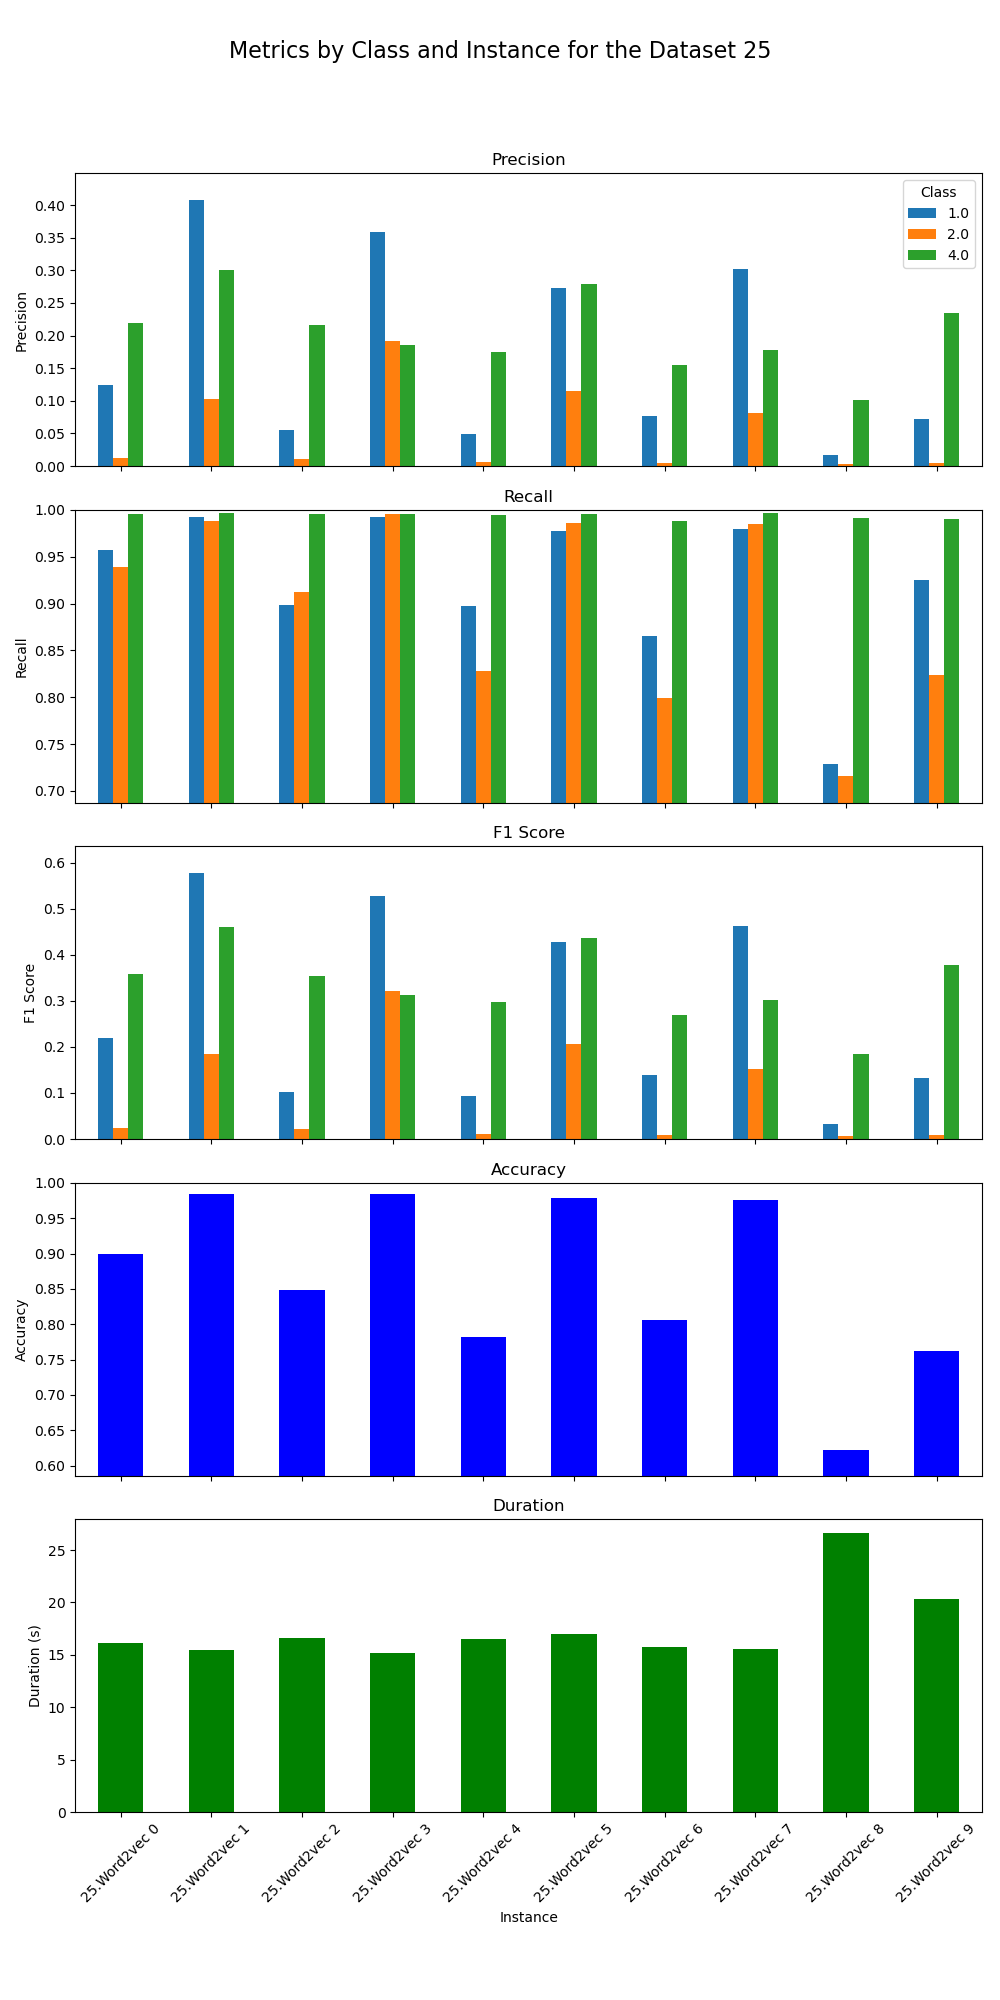
\includegraphics[width=0.6\textwidth]{img/annexes/25/25 - Metrics.png}
\caption{Metrics for the instances of the dataset 25}
\label{fig:25_metrics_instance}
\end{figure}

\begin{longtable}{|c|c|c|}
\caption{Word2vec 3 Classification Results on 25} \label{tab:25_word2vec_3_classifiers_results} \\
\hline
Class & Metric Name & Metric Value \\
\hline
\multirow{4}{*}{0.0} & Precision & 0.9999617471431186 \\
 & Recall & 0.9838132974079551 \\
 & F1 Score & 0.9918217959650952 \\
 & Support & 4437346.0 \\
 & Final Samples (after rebalancing) & 20964 \\
 & Initial Samples (before rebalancing) & 24506437 \\
\hline
\multirow{4}{*}{1.0} & Precision & 0.35848600570406536 \\
 & Recall & 0.9927710843373494 \\
 & F1 Score & 0.5267606634229499 \\
 & Support & 22410.0 \\
 & Final Samples (after rebalancing) & 20964 \\
 & Initial Samples (before rebalancing) & 125784 \\
\hline
\multirow{4}{*}{2.0} & Precision & 0.19214470284237725 \\
 & Recall & 0.9954484605087015 \\
 & F1 Score & 0.32211392679228934 \\
 & Support & 3735.0 \\
 & Final Samples (after rebalancing) & 20964 \\
 & Initial Samples (before rebalancing) & 20964 \\
\hline
\multirow{4}{*}{4.0} & Precision & 0.18481717011128776 \\
 & Recall & 0.9959839357429718 \\
 & F1 Score & 0.31177974269790054 \\
 & Support & 3735.0 \\
 & Final Samples (after rebalancing) & 20964 \\
 & Initial Samples (before rebalancing) & 20964 \\
\hline
\multirow{4}{*}{Macro Avg} & Precision & 0.4338524064502122 \\
 & Recall & 0.9920041944992445 \\
 & F1 Score & 0.5381190322195588 \\
 & Support & 4467226.0 \\
 & Final Samples (after rebalancing) & 83856 \\
 & Initial Samples (before rebalancing) & 24674149 \\
\hline
\multirow{4}{*}{Weighted Avg} & Precision & 0.9953868201030884 \\
 & Recall & 0.9838781382450765 \\
 & F1 Score & 0.9883602885462669 \\
 & Support & 4467226.0 \\
 & Final Samples (after rebalancing) & 83856 \\
 & Initial Samples (before rebalancing) & 24674149 \\
\hline
& Accuracy & 0.9838781382450765 \\ \hline
& True Positives & 22248 \\ \hline
& True Negatives & 4365520 \\ \hline
& False Positives & 39808 \\ \hline
& False Negatives & 140 \\ \hline
& AUC & 0.98 \\ \hline
& Duration (seconds) & 15.149247 \\ \hline
\end{longtable}


\subsection{26 chunk\_extraction (filtered entropy)}

\begin{figure}[H]
\centering
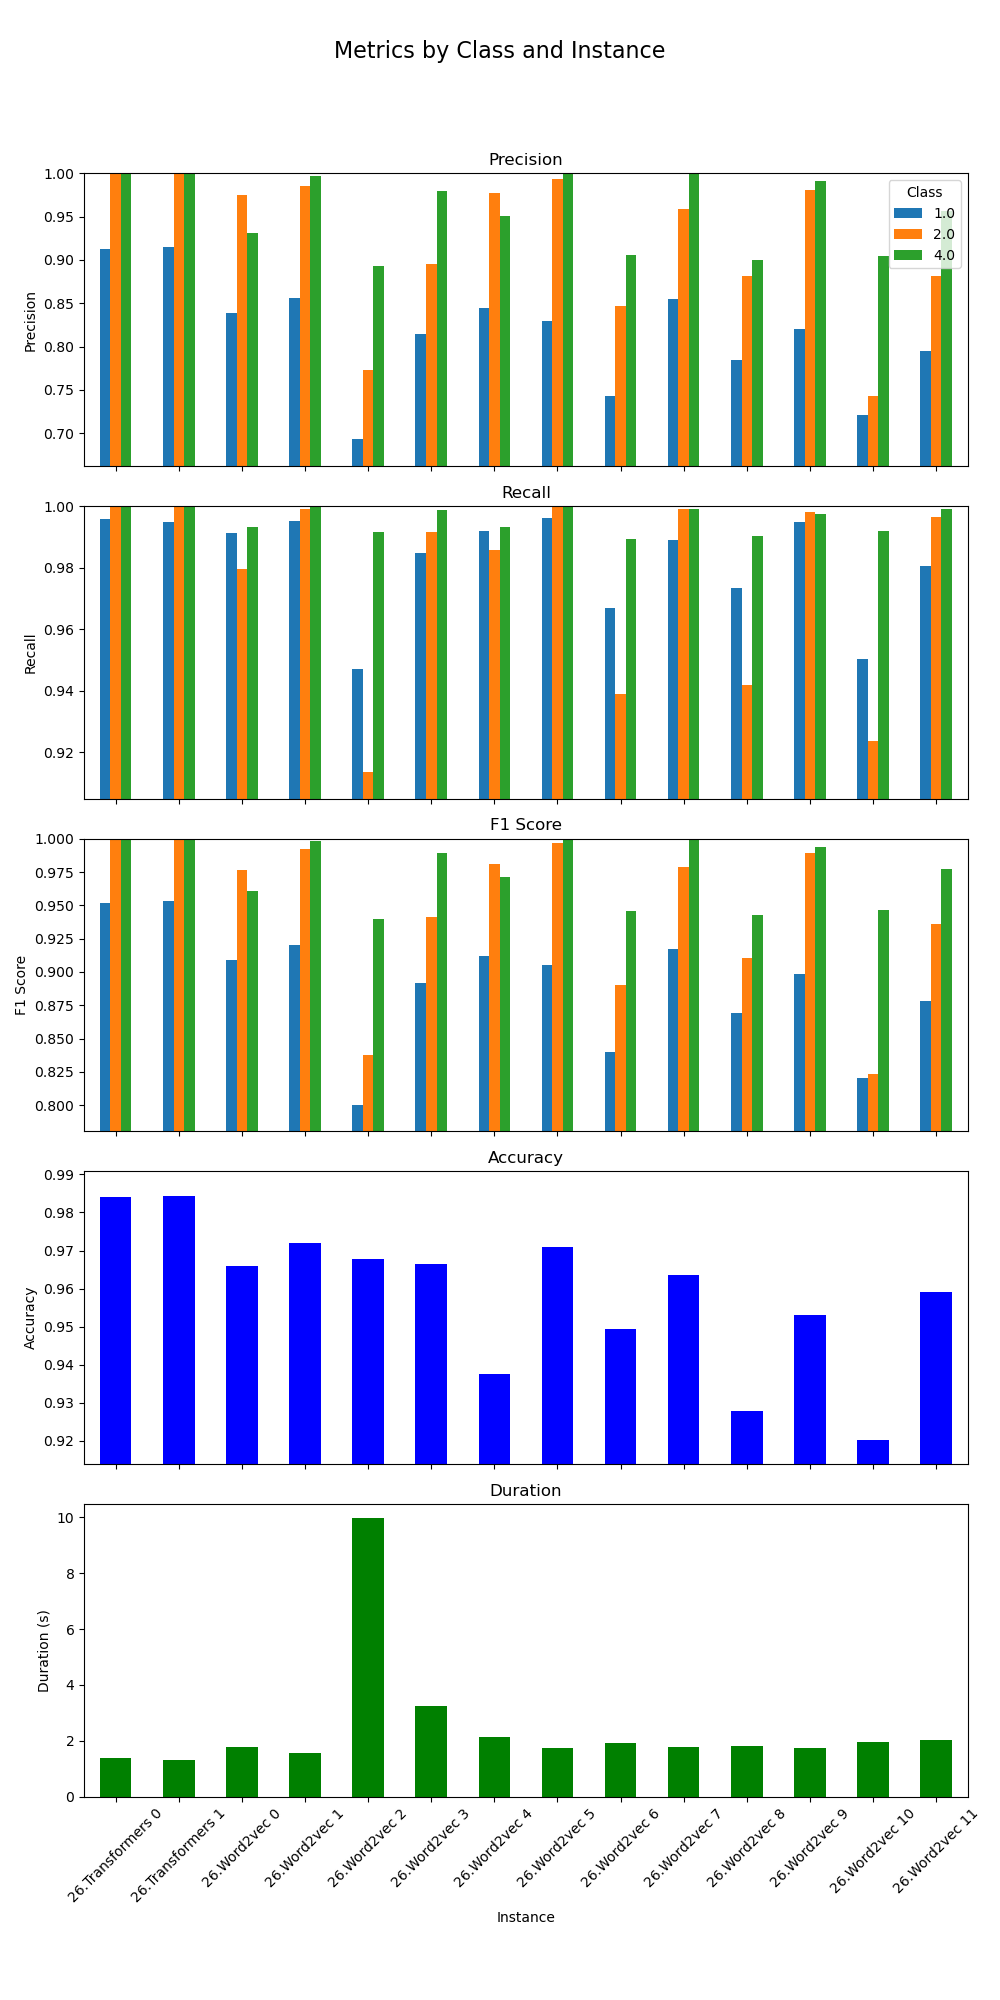
\includegraphics[width=0.6\textwidth]{img/annexes/26/26 - Metrics.png}
\caption{Metrics for the instances of the dataset 26}
\label{fig:26_metrics_instance}
\end{figure}

\begin{longtable}{|c|c|c|}
\caption{Transformers 1 Classification Results on 26} \label{tab:26_transformers_1_classifiers_results} \\
\hline
Class & Metric Name & Metric Value \\
\hline
\multirow{4}{*}{0.0} & Precision & 0.9989467459994826 \\
 & Recall & 0.9811611825985953 \\
 & F1 Score & 0.9899740882829596 \\
 & Support & 110198.0 \\
 & Final Samples (after rebalancing) & 20964 \\
 & Initial Samples (before rebalancing) & 620669 \\
\hline
\multirow{4}{*}{1.0} & Precision & 0.9148202855736091 \\
 & Recall & 0.9949129852744311 \\
 & F1 Score & 0.953187123252533 \\
 & Support & 22410.0 \\
 & Final Samples (after rebalancing) & 20964 \\
 & Initial Samples (before rebalancing) & 125784 \\
\hline
\multirow{4}{*}{2.0} & Precision & 1.0 \\
 & Recall & 1.0 \\
 & F1 Score & 1.0 \\
 & Support & 3735.0 \\
 & Final Samples (after rebalancing) & 20964 \\
 & Initial Samples (before rebalancing) & 20964 \\
\hline
\multirow{4}{*}{4.0} & Precision & 1.0 \\
 & Recall & 1.0 \\
 & F1 Score & 1.0 \\
 & Support & 3735.0 \\
 & Final Samples (after rebalancing) & 20964 \\
 & Initial Samples (before rebalancing) & 20964 \\
\hline
\multirow{4}{*}{Macro Avg} & Precision & 0.9784417578932729 \\
 & Recall & 0.9940185419682566 \\
 & F1 Score & 0.9857903028838731 \\
 & Support & 140078.0 \\
 & Final Samples (after rebalancing) & 83856 \\
 & Initial Samples (before rebalancing) & 788381 \\
\hline
\multirow{4}{*}{Weighted Avg} & Precision & 0.985544169072628 \\
 & Recall & 0.9843658533102986 \\
 & F1 Score & 0.9846234812939566 \\
 & Support & 140078.0 \\
 & Final Samples (after rebalancing) & 83856 \\
 & Initial Samples (before rebalancing) & 788381 \\
\hline
& Accuracy & 0.9843658533102986 \\ \hline
& True Positives & 22296 \\ \hline
& True Negatives & 108122 \\ \hline
& False Positives & 2076 \\ \hline
& False Negatives & 114 \\ \hline
& AUC & 0.93 \\ \hline
& Duration (seconds) & 1.309276 \\ \hline
\end{longtable}


\begin{longtable}{|c|c|c|}
\caption{Word2vec 1 Classification Results on 26} \label{tab:26_word2vec_1_classifiers_results} \\
\hline
Class & Metric Name & Metric Value \\
\hline
\multirow{4}{*}{0.0} & Precision & 0.9991360772271836 \\
 & Recall & 0.9655256901214178 \\
 & F1 Score & 0.9820433893737107 \\
 & Support & 110198.0 \\
 & Final Samples (after rebalancing) & 20964 \\
 & Initial Samples (before rebalancing) & 620669 \\
\hline
\multirow{4}{*}{1.0} & Precision & 0.8559530206494205 \\
 & Recall & 0.9951360999553771 \\
 & F1 Score & 0.9203119841531859 \\
 & Support & 22410.0 \\
 & Final Samples (after rebalancing) & 20964 \\
 & Initial Samples (before rebalancing) & 125784 \\
\hline
\multirow{4}{*}{2.0} & Precision & 0.9854766305782942 \\
 & Recall & 0.9991967871485944 \\
 & F1 Score & 0.9922892847646901 \\
 & Support & 3735.0 \\
 & Final Samples (after rebalancing) & 20964 \\
 & Initial Samples (before rebalancing) & 20964 \\
\hline
\multirow{4}{*}{4.0} & Precision & 0.9970635344367326 \\
 & Recall & 1.0 \\
 & F1 Score & 0.9985296083411309 \\
 & Support & 3735.0 \\
 & Final Samples (after rebalancing) & 20964 \\
 & Initial Samples (before rebalancing) & 20964 \\
\hline
\multirow{4}{*}{Macro Avg} & Precision & 0.9594073157229077 \\
 & Recall & 0.9899646443063473 \\
 & F1 Score & 0.9732935666581793 \\
 & Support & 140078.0 \\
 & Final Samples (after rebalancing) & 83856 \\
 & Initial Samples (before rebalancing) & 788381 \\
\hline
\multirow{4}{*}{Weighted Avg} & Precision & 0.9758098498505534 \\
 & Recall & 0.972079841231314 \\
 & F1 Score & 0.972880234960717 \\
 & Support & 140078.0 \\
 & Final Samples (after rebalancing) & 83856 \\
 & Initial Samples (before rebalancing) & 788381 \\
\hline
& Accuracy & 0.972079841231314 \\ \hline
& True Positives & 22301 \\ \hline
& True Negatives & 106399 \\ \hline
& False Positives & 3750 \\ \hline
& False Negatives & 92 \\ \hline
& AUC & 0.92 \\ \hline
& Duration (seconds) & 1.557051 \\ \hline
\end{longtable}


\subsection{27 chunk\_extraction (filtered entropy and chunk size)}

\begin{figure}[H]
\centering
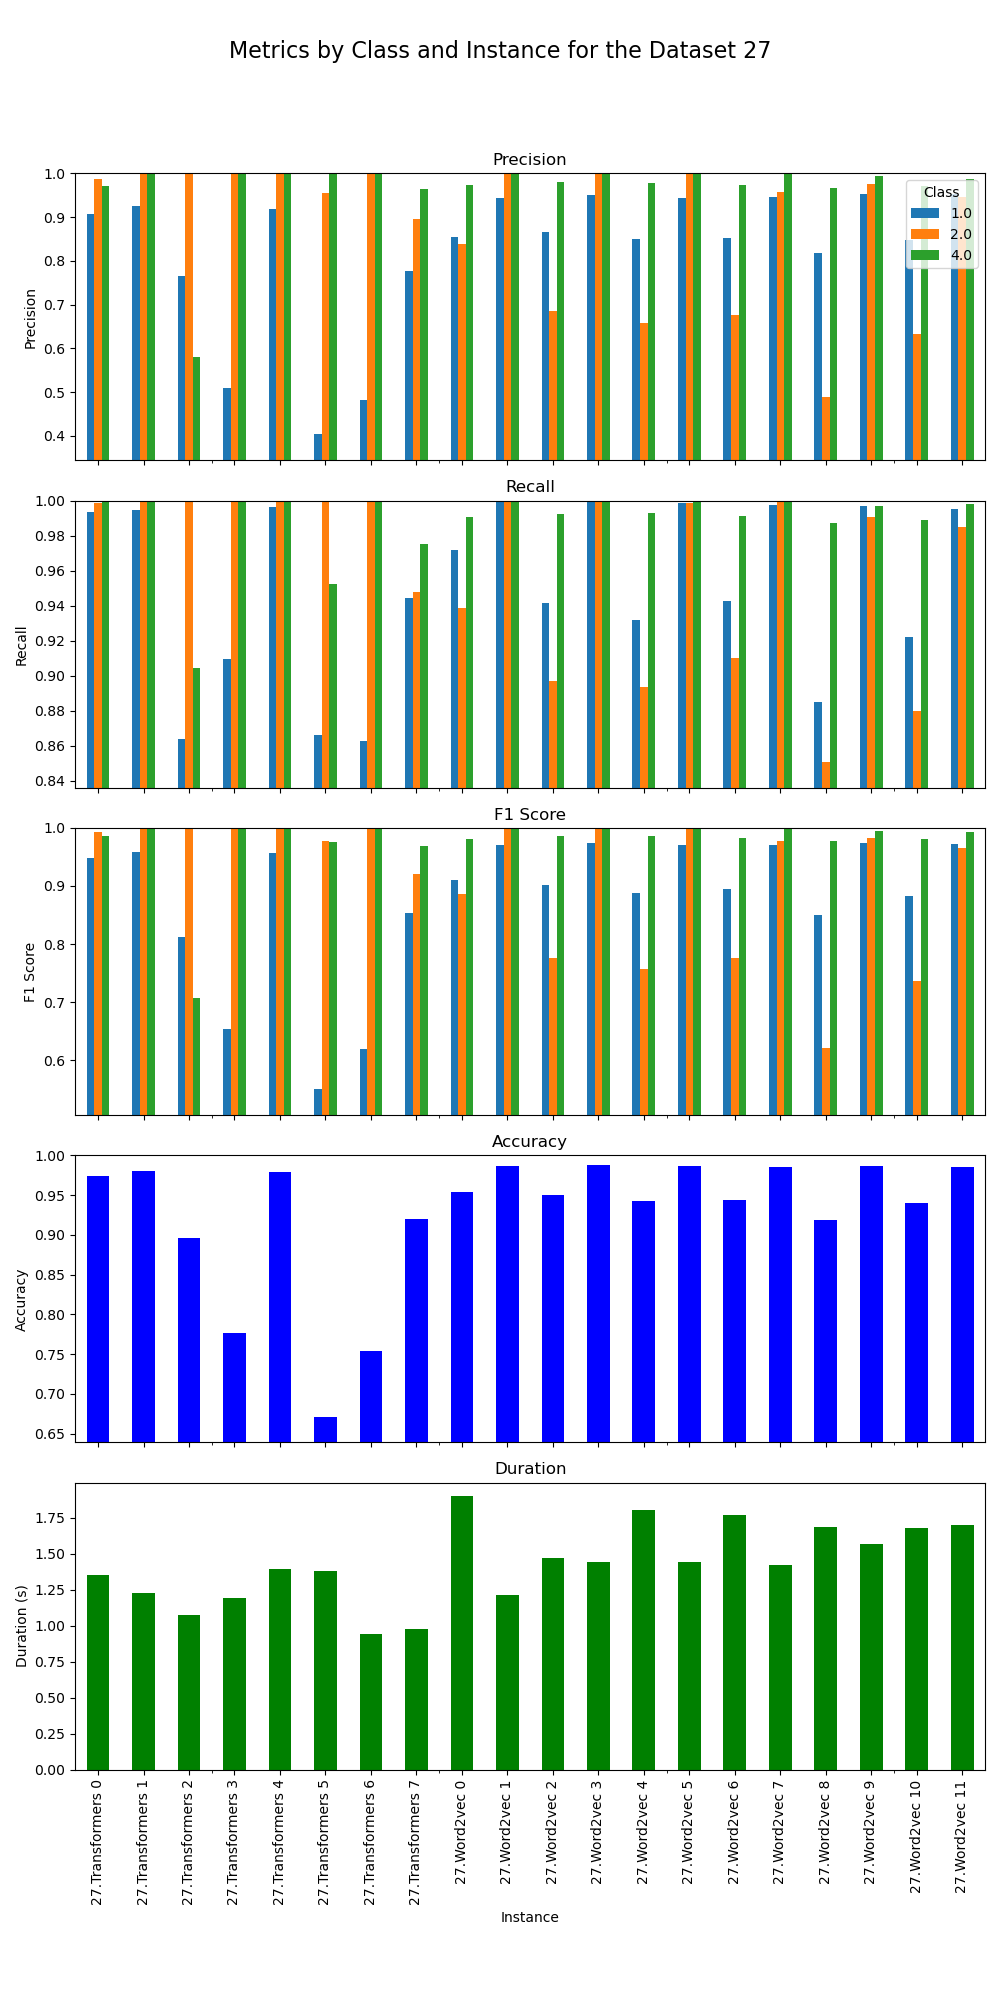
\includegraphics[width=0.6\textwidth]{img/annexes/27/27 - Metrics.png}
\caption{Metrics for the instances of the dataset 27}
\label{fig:27_metrics_instance}
\end{figure}

\begin{longtable}{|c|c|c|}
\caption{Transformers 1 Classification Results on 27} \label{tab:27_transformers_1_classifiers_results} \\
\hline
Class & Metric Name & Metric Value \\
\hline
\multirow{4}{*}{0.0} & Precision & 0.9981469570277803 \\
 & Recall & 0.9728055642621531 \\
 & F1 Score & 0.9853133479973091 \\
 & Support & 66999.0 \\
 & Final Samples (after rebalancing) & 20964 \\
 & Initial Samples (before rebalancing) & 376160 \\
\hline
\multirow{4}{*}{1.0} & Precision & 0.9244328314877027 \\
 & Recall & 0.9946006247211067 \\
 & F1 Score & 0.958233915865953 \\
 & Support & 22410.0 \\
 & Final Samples (after rebalancing) & 20964 \\
 & Initial Samples (before rebalancing) & 125784 \\
\hline
\multirow{4}{*}{2.0} & Precision & 0.9997323340471093 \\
 & Recall & 1.0 \\
 & F1 Score & 0.9998661491098916 \\
 & Support & 3735.0 \\
 & Final Samples (after rebalancing) & 20964 \\
 & Initial Samples (before rebalancing) & 20964 \\
\hline
\multirow{4}{*}{4.0} & Precision & 1.0 \\
 & Recall & 0.9997322623828648 \\
 & F1 Score & 0.9998661132681751 \\
 & Support & 3735.0 \\
 & Final Samples (after rebalancing) & 20964 \\
 & Initial Samples (before rebalancing) & 20964 \\
\hline
\multirow{4}{*}{Macro Avg} & Precision & 0.9805780306406481 \\
 & Recall & 0.9917846128415311 \\
 & F1 Score & 0.9858198815603322 \\
 & Support & 96879.0 \\
 & Final Samples (after rebalancing) & 83856 \\
 & Initial Samples (before rebalancing) & 543872 \\
\hline
\multirow{4}{*}{Weighted Avg} & Precision & 0.9812280060199797 \\
 & Recall & 0.9799337317684947 \\
 & F1 Score & 0.9801714618958681 \\
 & Support & 96879.0 \\
 & Final Samples (after rebalancing) & 83856 \\
 & Initial Samples (before rebalancing) & 543872 \\
\hline
& Accuracy & 0.9799337317684947 \\ \hline
& True Positives & 22289 \\ \hline
& True Negatives & 65177 \\ \hline
& False Positives & 1822 \\ \hline
& False Negatives & 121 \\ \hline
& AUC & 0.89 \\ \hline
& Duration (seconds) & 1.23036 \\ \hline
\end{longtable}


\begin{longtable}{|c|c|c|}
\caption{Word2vec 3 Classification Results on 27} \label{tab:27_word2vec_3_classifiers_results} \\
\hline
Class & Metric Name & Metric Value \\
\hline
\multirow{4}{*}{0.0} & Precision & 0.9997874343323919 \\
 & Recall & 0.9828206391140166 \\
 & F1 Score & 0.9912314373668721 \\
 & Support & 66999.0 \\
 & Final Samples (after rebalancing) & 20964 \\
 & Initial Samples (before rebalancing) & 376160 \\
\hline
\multirow{4}{*}{1.0} & Precision & 0.9511148863877681 \\
 & Recall & 0.9992860330209727 \\
 & F1 Score & 0.9746055924273745 \\
 & Support & 22410.0 \\
 & Final Samples (after rebalancing) & 20964 \\
 & Initial Samples (before rebalancing) & 125784 \\
\hline
\multirow{4}{*}{2.0} & Precision & 0.9991972170189992 \\
 & Recall & 0.9997322623828648 \\
 & F1 Score & 0.9994646680942185 \\
 & Support & 3735.0 \\
 & Final Samples (after rebalancing) & 20964 \\
 & Initial Samples (before rebalancing) & 20964 \\
\hline
\multirow{4}{*}{4.0} & Precision & 1.0 \\
 & Recall & 1.0 \\
 & F1 Score & 1.0 \\
 & Support & 3735.0 \\
 & Final Samples (after rebalancing) & 20964 \\
 & Initial Samples (before rebalancing) & 20964 \\
\hline
\multirow{4}{*}{Macro Avg} & Precision & 0.9875248844347898 \\
 & Recall & 0.9954597336294635 \\
 & F1 Score & 0.9913254244721164 \\
 & Support & 96879.0 \\
 & Final Samples (after rebalancing) & 83856 \\
 & Initial Samples (before rebalancing) & 543872 \\
\hline
\multirow{4}{*}{Weighted Avg} & Precision & 0.9885139661056759 \\
 & Recall & 0.9879437236139927 \\
 & F1 Score & 0.9880410298802881 \\
 & Support & 96879.0 \\
 & Final Samples (after rebalancing) & 83856 \\
 & Initial Samples (before rebalancing) & 543872 \\
\hline
& Accuracy & 0.9879437236139927 \\ \hline
& True Positives & 22394 \\ \hline
& True Negatives & 65848 \\ \hline
& False Positives & 1150 \\ \hline
& False Negatives & 14 \\ \hline
& AUC & 0.89 \\ \hline
& Duration (seconds) & 1.442202 \\ \hline
\end{longtable}


